% !Mode:: "TeX:UTF-8:Hard"
\ifx \allfiles \undefined
\documentclass[a4paper,12pt,twoside]{book}
%\usepackage{CJKutf8}
\usepackage[T1]{fontenc}
\usepackage{pifont}
\usepackage{graphicx}
\usepackage{capt-of}
\usepackage{color}
\newcommand{\linuxcommand}[1]{\texttt{\textcolor{blue}{\$ #1 \Pisymbol{psy}{191}}}}
\newcommand{\op}[1]{\textcolor{blue}{-#1}}
\newcommand{\hotkey}[1]{\framebox{#1}}
\newenvironment{screen}{\sffamily}{\rmfamily}

\usepackage{listings}
\definecolor{mygray}{rgb}{0.9,0.9,0.9}
\lstset{backgroundcolor=\color{mygray}, basicstyle=\small}
\lstset{morecomment=[s][\color{red}]{/*-}{*/}}
\newcommand{\Hilight}[1]{\makebox[0pt][l]{\color{yellow}\rule[-3pt]{#1em}{11pt}}}
\newcommand{\HilightLine}[2][yellow]{\makebox[0pt][l]{\color{#1}\rule[-4pt]{#2em}{13.9pt}}}


\begin{document}
%\begin{CJK*}{UTF8}{song}
\title{Basic Knowledge}
\author{Yan Zhao}
\date{}\maketitle

\tableofcontents

\else
\chapter{Developing Knowledge and Tool}
\fi

\section{Linux basic}
\begin{itemize}
		\item There is a good article to introduce Linux distribution. \textbf{The name is "RedHat vs Debian : Administrative Point of View".} You can google and read it. In one word. RedHat is stable, commercial server with small amount of packages. Fedora and CentOS are based on it. Fedora is cutting edge implementation(For test). Another big group is Debian, It's also stable with much more packages. Ubuntu is based on Debian.

		\item Ubuntu is mostly for desktop, and Mint is sleek and quick version of Ubuntu, CentOS is for server, It's more stable. \textbf{If you use virtual machine, recommend Mint, if you want to install linux directly on a computer, you can use Ubuntu system.}, because it's more friend toward beginner and PC. 

		\item There are two Interface Framework, Qt and GTK\@.  KDE is based on QT, and Gnome and Cinnamon(Mint) is based on GTK.  

		\item You can use \linuxcommand{uname} to check basic information about your computer, detail can be seen uname --help. The processor type (or name) refers for what architecture has been made the processor.  The hardware machine name must be compatible with the processor type, in other words, must be the same type as the processor type.  And finally, the hardware platform refers to the whole instructions that the hardware uses to process and which it needn't be a higher version than the processor type. i686=x86\_64

		\item \linuxcommand{lscpu} will tell you how many cores do you have. Socket is physics CPU, "cores per socket" is number of cores. 
\end{itemize}

\section{Shell}
\subsection{Shell type}
\begin{itemize}
		\item There are two basic shell, one is bash and the other is tcsh. They can be change by calling \linuxcommand{bash} or \linuxcommand{tcsh}.  You can use echo \$0 to see which shell you are using right now.

		\item By now, a new shell is zsh, It support more features. 

		\item You can use \linuxcommand{chsh}, -l will list all available shell, and -s follow new shell full path name, such as \linuxcommand{chsh -s /bin/bash}.

		\item Every time when you open a new terminal, It will read .bashrc or .rshrc. It depends on what shell you are using, that is why you need to use \linuxcommand{echo \$0} to know which shell you are using. It will use export(bash) or setenv(csh) to load all envoriment variable. 

		\item In tcsh, you can use bindkey -e and bindkey -v to change to emacs mode and vi mode.In bash, you can use set -o vi or set -o emacs.

		\item Once in vim mode, It's important to distinguish insert mode and command mode. For bash( version 4.3 or 4.4) you can use  "set show-mode-in-prompt on" in .inputrc file. For zsh, you also can implement it. But in tcsh, there isn't any good way to show message on prompt. Just accept it.   
\end{itemize}

\subsection{wild character and quote}
\begin{itemize}
		\item Single quotes preserves the literal value of each character.  Double quotes preserves the literal value of all characters within the quotes, with the exception of '\$', 'backtick', '$\backslash$', and, when history expansion is enabled, '!'. 
\begin{verbatim}
echo '$PATH `pwd` '
echo "$PATH `pwd` \$PATH"
\end{verbatim}
		\item For shell, There are "*, ?, [ ] and \{\}" wild character. \textbf{Any time you input these four wild characters, shell will interpret it according to all the files names.}

		\item \{\} will not match file name, echo a\{.h,.c\} just output a.h and a.c \textbf{Don't use space inside \{\} }.

		\item For example echo [a-d]c.  
				\begin{enumerate}
						\item shell see [ ], it will expand according to file names. If it doesn't match, it will print No match. If there are bc file or dc file. [a-d]c will be expanded to "bc dc".
						\item Then shell invoke echo command.
				\end{enumerate}

		\item For \{\}, You use \linuxcommand{echo \{*.txt,*.c\}}. \textbf{No space after comma.} It will expanded to a.txt b.c if there is a.txt and b.c in your directory.

		\item If you don't want shell to interpret wild character, use $\backslash$

		\item A good example of wild character is \linuxcommand{grep --exclude=a$\backslash$*.h 'a*b' *.h}. You should know three * meaning in previous command.
\end{itemize}

\subsection{Environment variable}
\begin{itemize} 
		\item When bash is invoked as an interactive login shell, or as a non-interactive shell with the --login option, it first reads and executes commands from the file /etc/profile, if that file exists. Then/etc/profile.d/*.sh. Then it looks for ~/.bash\_profile,  ~/.bash\_login, and ~/.profile, in that order, and reads and executes commands from the first one that exists and is readable. The --noprofile option may be used when the shell is started to inhibit this behavior.
		
		\item When an interactive shell that is not a login shell is started, bash reads and executes commands from  /etc/bash.bashrc and ~/.bashrc, if these files exist. This may be inhibited by using the --norc option. The --rcfile file option will force bash to read and execute commands from file instead of /etc/bash.bashrc and  ~/.bashrc.	

		\item For tcsh, read .cshrc file, for zsh, read .zshrc file.

		\item This goes pretty far back in the Unix history. rc stands for "run commands", and makes sense actually.

		\item echo \$0 will show "bash", it's not login shell. If it shows "-bash", it is login shell.  
	
		\item Why we need variable, just like macro in C language. With variable, we can configure and customize an application outside. And we can customize a variable to affect a lot of applications. Such as \$PATH.
				
		\item For different shell, you have different syntax in shell script. For example, for bash shell you can use YanVar=123, There is no space between =.You also can use unset command "unset YanVar". Or use check command: \linuxcommand{echo \$YanVar}. Different shell have different syntax, tcsh muse use set. \textbf{Pay attention, in shell, there is no variable, just macro, so expansion is key idea to understand it's behaviour. Such as expansion order}.

		\item There are two kinds of variables: environment and user defined.

		\item \linuxcommand{env} shows all the environment variable. Such as \$HOME,  \$PATH, \$LANG,\$EDITOR which can specify you default editor in your system.\linuxcommand{set} list all the local environment variables and user defined variable , that is more than env command. For example, the \$PS1.  

		\item \linuxcommand{getconf} can get some system variable, such as \linuxcommand{getconf ARG\_MAX}, you can use xargs -n 50 to make command satisfy the ARG\_MAX
	
		\item In mint, maybe in your home directory, there is no .bashrc file, so you need to create one and add export PATH=\$PATH:/home/yan/openuh-install/bin  then exit the current terminal and restart a new one. Then use echo \$PATH to see if the directory has been added.
	
		\item In previous command, Linux use ":" but windows use ";" why windows use different?  
			
		\item If you already in terminal, you can use "export" or "setenv" command to add environment variable. If these commands are in a sh file, you have to use \linuxcommand{source a.sh} to run. Because, if no source command, it will open a child terminal, so after a.sh finish, child terminal will disappear, and all the environment variable you just set in the child terminal will disappear too. 

		\item If There is only one environment variable need to be set, you can run setenv or export in your current shell directly, then you can run a command, this command will be run in the child process, but child process can access parent environment variable, it's OK
				
		\item \linuxcommand{export DEPART=Sale} and \linuxcommand{DEPART=Sale ; export DEPART} they means the same. 

		\item \linuxcommand{setenv} is csh command. In bash, you can use \linuxcommand{export} directly. \textbf{csh doesn't use =, bashrc doesn't use backslash.}
\begin{verbatim}
in .cshrc
setenv PATH $PATH\:/users/yzhao4/python-3.23/bin

in .bashrc
export PATH=$PATH:/storage/yzhao/binexport 
\end{verbatim}

		\item If There are a few environment variables need to be set, You'd better put them into a script file. \textbf{But you have to use source a.sh} to make sure a.sh running in the current process, not a child process. 

		\item Two shells don't share history and environment variables. 
\end{itemize}
	
\subsection{pipe}
\begin{itemize}
		\item pipe command can be called "filter", It will accept input from STDIN, perform operations, then send it to STDOUT. Such as \textbf{grep, uniq, sort, fmt, pr, head, cut, tee, tr, join, paste, expand, split, tr, awk, sed, less}

		\item You can't judge if a command is filter by running it. "cat" will hang up to wait for you from STDIN, but less will show error message.

		\item xargs is also a filter, you can use this way \linuxcommand{find . -name "*.c" | xargs rm -rf } a.c and b.c will be rm command arguments.

		\item Sometimes, a command need a file name as input or output, but you don't want to give a filename, It usually used in pipe commands, such as \linuxcommand{gzip -dc a.tar.gz  | tar -xvf  - }. It just like \linuxcommand{gzip -dc a.tar.gz  | tar -xvf  /dev/stdin}

  \item "-" has nothing with shell, It's only available in tar command. Most of time, It's only used in tar. 
\end{itemize}

\subsection{shell script}
\subsubsection{Basic}
\begin{itemize}
		\item The first line of script is \verb=#!/bin/bash=.  This is a special clue given to the shell indicating what program is used to interpret the script. Other scripting languages such as perl, awk, tcl, Tk, and python can also use this mechanism.

		\item After you finished script file, use \linuxcommand{chmod +x your-script-name}.

		\item echo -e "aaa$\backslash$nbbb" will output two lines.

		\item \linuxcommand{!!} run the previous command, \linuxcommand{!\$} is the previous argument. \linuxcommand{\$?} is the last bash command result, If it's 0, means that everything is OK. Detail can be found in google "Become a Command Line Ninja With These Time-Saving Shortcuts''

		\item \linuxcommand{command1;command2}.   To run two command with one command line.  \linuxcommand{command1 \&\& command2} command2 is executed if, and only if, command1 returns an exit status of zero. \linuxcommand{command1 || command2} command2 is executed if and only if command1 returns a non-zero exit status.

\end{itemize}

\subsubsection{Variable} 

\begin{itemize}
\item In script file, \$0 is script name, and \$1, \$2.. are arguments to the scripts. 

\item print the contains of variable (HOME) and not the HOME. You must use \$ followed by variable name to print variable. \verb= echo $HOME= print the variable contents. And \verb=echo HOME= just print "HOME" string. It's a little confused for a C programmer, but you need to be used to it. 

 \item In most cases, \$var and \$\{var\} are the same.  The braces are only needed to resolve ambiguity in expressions: such as echo \$\{var\}bar

\item \$(command) is same as `command. 

\end{itemize}

\subsection{Terminal tips}

\begin{itemize}

		\item Motion shortcut keys are list below: Ctrl+p or up down arrow key can go to the previous command, this is very useful. 
\begin{center}
  \begin{tabular}{c|c}
 \hline shortcut & function \\
\hline Ctrl+f,b & forward, backward character \\
\hline alt+f,b & forward, backward word \\
\hline Ctrl+a,e & move start,end \\
\hline Ctrl+p,n & previous, next line \\
\hline Ctrl+r & search command history \\
 \hline
  \end{tabular}
\end{center}

		\item delete shortcut keys: You can use "hw" to delete previous character or word. "dd" use to delete forward character or word, "uk" to sentence beginning and end. In Vim, the keyboard shortcut is not the same. \textbf{They are bash edit keyshortcut.}

\begin{center}
  \begin{tabular}{|c|c|}
 \hline shortcut & fucntion \\
 \hline \textbf{Ctrl+l} & clear the screen \\	
\hline ctrl+k,u & delete to begin/end \\
\hline alt+d ctrl+w & delete forward/backward word \\
\hline Ctrl+d,h  & delete forward/backward a character  \\
 \hline
  \end{tabular}
\end{center}

		\item You can remember "eu" "ak". They both delete the whole line, The first letter is move command. And the second letter is edit command. 

		\item \linuxcommand{bind -p} will list all the shortcut. This is bash command. In tcsh shell, you can use \linuxcommand{bindkey -v} to make your commad line edit function compatible with VI. Also use esc to switch command mode and insert mode. For example, by press Esc, then, you can use fx command to jump x character in the command line. It's very convince for edit long command line.

		\item  About keyboard shortcut, I have good idea, that is to use left Ctrl and Alt together, because you can use your thumb to press Alt and use palm to press Ctrl\_L,(Even in my three laptops, I also can press Ctrl\_L easily by palm).
	So a shortcut can be defined below:
	\[ \left\{ \begin{array}{cl}
	            \textrm{move} & \left\{ \begin{array}{c} \textrm{other: Ctrl\_L} \\ \textrm{emacs: Alt\_L} \end{array}  \right. \\
		    \textrm{select} & \left\{ \begin{array}{c} \textrm{other: Ctrl\_L+Shift\_L} \\ \textrm{emacs: Alt\_L+Shift\_L} \end{array}  \right. \\
	           \end{array} \right. + \left\{ \begin{array}{c}
						\textrm{left character: J} \\
						\textrm{right character: L}\\
						\textrm{upward: I}\\
						\textrm{downward: k}\\
						\textrm{left word: U}\\
						\textrm{right word: O} \\
						\textrm{begin line: H}\\
						\textrm{end line: ;}\\
						\end{array} \right.
	\]
	Delete command is below: \\
	\[ \textrm{delete} \left\{ \begin{array}{l}
	            \textrm{left character: Backspace}  \\
		    \textrm{right charcter: Ctrl\_L+N} \\
		     \textrm{left word: Ctrl\_L+Backspace}  \\
		    \textrm{right word: Ctrl\_L+M} \\
		     \textrm{line: Ctrl\_L+P}  \\
	           \end{array} \right.
	\]
	

	Question 1: why always left Ctrl?  \\
	Answer: Now, if you are smart enough, you can found that there is rules inside. All the commands is left Ctrl add right hand character, becuase left Ctrl can be
	pressed by left palm and right hand is more flexible than left hand when you click the different character. \\

	Question 2: why other use Ctrl and Emacs use Alt. \\
	Answer: In common applications, Alt has been assign to trigger menu item, such as Alt+F will trigger File menu, so, I must use Ctrl. In Emacs, on the contrary,
	Ctrl has been used to trigger some common commands, so I use Alt key( and Alt is used not often as Ctrl).\\

	Question 3: How can I export my custom shortcut to other computers \\
	Answer: There are two kind of shortcut one is kate and other is kile, they store in \verb=.kde/share/apps/katepart/katepartui.rc= and \linebreak[4] \verb=.kde/share/apps/kile/kileui.rc=
	you can copy them and cover them in your computer. If version is different, Maybe it's a little difficult. But you can just do it within the application, it don't need very long time. \\
        \\
	By now, these customized shortcuts haven't been used in practical use. Anyway, you can use arrowkey, it don't need too much memory. But it is a good suggestion. You can learn how to define a customized shortcut. If you need to do a lot texting job, they are very useful.
	 %目前,这些键盘的定义我还没有在实践中使用过。毕竟,用箭头键太直接了,而按住ctrl在一些笔记本上不是太方便。 不过,他们依旧是一个很好的建议,以后当你使用大键盘,或者是比较密集的进行编辑工作的时候,还是非常值得尝试一下的。
  \item Ctrl+Alt+F1\ldots F6 switch terminal. Ctrl+Alt+F7 return back to GUI\@. When F7 doesn't work, you can try F8. 
\end{itemize}


\subsection{Time}
\begin{itemize}
		\item For Linux file time: there are three time stamps: atime (access time), it is when the file was last read.\  ctime is the inode change time, while mtime is the file modification time.\  mtime changes when you write to the file. It is the age of the data in the file. \textbf{Whenever atime or mtime changes, so does ctime, except you use touch command} But ctime changes a few extra times. For example, it will change if you change the owner or the permissions on the file.  

		\item  timestamp will be used in many linux commands, ls -l will show modification time. and you can use \linuxcommand{stat fileName} to see all the three time. The can be used in find command. 

		\item atime sometimes will not updated by visiting a file. Atime updates are by far the biggest IO performance deficiency that Linux has today. So sometimes it's disable when mount in option in /etc/fstab

		\item \linuxcommand{touch} can change time of a file or you can use it to produce an empty file.  \linuxcommand{touch -a existFile} change access time and ctime. \linuxcommand{touch -t existFile} change modify time and ctime.   \linuxcommand{touch -c existFile} change a,c and m time. 
            
		\item \linuxcommand{touch -t YYMMDDHHmm} will set mtime and atime to the date you want and it sets ctime to \textbf{NOW}. You have complete control over mtime, but the system stays in control of ctime. So mtime is a little bit like the date on a letter while ctime is like the postmark on the envelope. System use ctime to do backup job. An example can be found in my evernote book mark. 

\end{itemize}


\section{File and Dir}
\subsection{Basic}
\begin{itemize}
		\item A hard link points to the file by \textbf{inode}.  A symbolic link points to the file by \textbf{filename}. 
 
		\item  There is no "real" hard link name; All hard links are equally valid names for the file. You can use \linuxcommand{ls -l}. The first number after the file mode is the link count(this count is represent hard link number).  For symbolic link, It just point to a filename, If origin file name changed, symbolic link will not be valid.   symbolic link is very flexible,  It can be linked to a dir or it can be linked to different file system. But hard link has many restriction.  
		\item \linuxcommand{find -L / -samefile path/to/foo.txt}find all files links to foo.txt

		\item Absolute directory must begin with root directory /.
		
		\item Linux doesn't use extension name to specify file type, you should use \linuxcommand{file fileName} to judge it.  

		\item When you use ls -l, the first character stands for different kinds: -:file, d:Dir, l:link file, b:interface of device. So you can use \linuxcommand{ls -al | grep \^{}d} to show all the directories. 
	 
		\item \linuxcommand{ls -d */} will list only directory without all files in it. if you want to see all files in it. omit -d
 
		\item /usr stands for UNIX Software Resource, isn't users directory. It associate with software. /users includes all the users name, don't confuse them. FHS recommend linux developer install their application into the different dirs inside of /usr:  such as /usr/bin and /usr/lib. Don't build their separately directory.  For example, when you install codeblock, you can see codeblock exe file in /usr/bin. When you use \linuxcommand{ldd codeblock}. you can see it use a lot of lib in /usr/lib. There is no codeblock directory which includes everything.  It's different with Window system.
		   	
         \item /var include all cache, log, mail which are increased when you system is running. so it will increase with time. 
         
		 \item The Dir Structure:
\begin{center}
\begin{tabular}{p{0.2\textwidth}|p{0.7\textwidth}}
  \hline
  % after \\: \hline or \cline{col1-col2} \cline{col3-col4} ...
  /bin & includes important comands: mv, mkdir, chmod, cat, chown and date  \\
 \hline  /etc & Main configuration file: /etc/init.d/ /etc/fstab \\
  \hline /home & home directory \\
  \hline /opt & just like /usr/local  \\
  \hline /usr & /usr/local install some your own software, /usr install OS software.  /usr/bin, /usr/include(c++ language), /usr/lib(c++ language),  /usr/src \\
  \hline /tmp & any body can access or write it.     \\
  \hline /srv & web service(www and ftp) access data \\
  \hline /sbin & root command \\
  \hline /proc and /sys & virtual file system, they are stored in memory.  proc and kernerl information \\
  \hline /dev & device file \\
  \hline /lib & lib used when you start linux. /lib/modules has kernel modules \\
  \hline 
\end{tabular} 
 \end{center}
\end{itemize} 

\subsection{partition and mount point}
	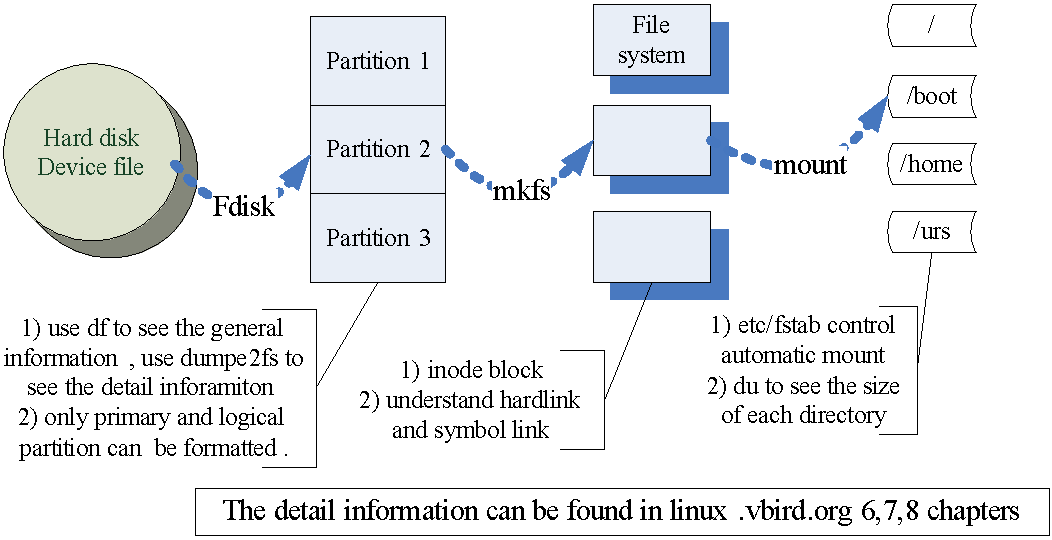
\includegraphics[scale=0.8]{pics/basic_file_system_clip}
\begin{itemize} 
		\item A good tool software in linux system is GParted, which  is used for creating, deleting, resizing, moving, checking, and copying disk partitions and their file systems.  You also can use df command to check your system \textbf{partitions}. You can create 1) partitions by GParted 2) mkdir a dir 3) then mount them by adding below text in /etc/fstab file. \verb=/dev/sda3 /home/yan/llvm ext4 defaults 0 0=
   
		\item \textbf{/etc, /bin, /dev, /lib and /sbin can NOT be put in different partition with root /. }  
\end{itemize}

\subsection{Permission or file mode}
\begin{itemize}
		\item \linuxcommand{ls -al} will list all the files ownership and permission. Basically, all the system support \linuxcommand{ll} command directly. 
			  
		\item There are three different groups: owner, Group, and Other. In each group,  there are three different permissions: r, w, x;

		\item For File and Dir, "rwx" has different meaning. x for Dir means you can come into this dir.  For a Dir, if you only have r permission, you only can \linuxcommand{ls -l Dir}, You can't cp a file from it unless you have x permission. So x permission is very important for a Dir
		  	
		\item \linuxcommand{chown chgrp} are very useful when you copy files to other peoples. \linuxcommand{chgrp -R grpName dirName}, you must make sure grpName in /etc/group file. or it will report error.  \linuxcommand{chown} command need to make sure owner name in /etc/passwd file. 

          \item When you need to use chgrp or chown? When you copy a file to other people. 

		  \item \linuxcommand{chmod} command follow[ugoa][+-=][rwx], for example, \linuxcommand{chmod u+x file}  or \linuxcommand{chmod go=r file}. There are four letters: u(owner), g(group), o(other) and a(all).\textbf{u represent owner, You need to remember that specially}. ("=") means "set the permissions exactly like this.
				  
		  \item SUID or GUID, In simple words users will get file owner’s permissions as well as owner UID and GID when executing a file/program/command. An good example is passwd command, It's owned by root, When you launch it, you have root permission to modify /etc/shade file. That is all!
\end{itemize}


\subsection{Commands about File}
\begin{itemize}
		\item \linuxcommand{du -h} command displays the sizes in kilobytes of all files in the specified directory.  df command displays the amount of unused space left in your disk system. \linuxcommand{du -sh *} will show your every directory size. \linuxcommand{du -sh * | sort -h} will sort all directory size. Don't use sort -n here, it will put 1.1G ahead 1.2M. 

		\item \linuxcommand{pwd} return where you are

		\item \linuxcommand{cd -} will return the previous path

		\item \linuxcommand{diff a.cpp b.cpp} will show line-by-line differences. 

		\item when you run a command, sometimes you need to \linuxcommand{./a.out}. "./" means current directory.
		
		\item When you use cp, you need pay attention to -a options, it related to maintains permission and owners.

        \item You can use \linuxcommand{od} to see the binary file, It reminds me the UltraEdit
        
        \item \linuxcommand{rmdir} only can be used to delete an empty dir. You can use rm -r to delete a directory with files in it.

		\item \linuxcommand{tail, head, cat ,tac, less } less will stop, to ask you to continue. Maybe less is better than cat.  I often copy-and-paste text from the web into a file like this (command prompt shown):
                \begin{verbatim}
                $ cat > filename
                <Cmd-V>
                <Ctrl-D>
                \end{verbatim}
		\item \linuxcommand{which -a command} will help you find command's name and in all \$PATH directory.  \linuxcommand{type} can tell you if a command is bash build in command. Such as cd command.  They are used to know more about your commands
		\item \linuxcommand{file} is to determined the kind of all files.( executable, text, or data file).  
                
		\item \linuxcommand{locate} can help you find a file very quickly, because it just search in an index database.   You can use \linuxcommand{updatedb} to update this database. \linuxcommand{whereis} just look for binary(-b option) or source(-s option) files. They just used to search binary and source files.  
\end{itemize}

\subsection{Find command}
\begin{itemize}
		\item \linuxcommand{find . *.txt} and \linuxcommand{find . "*.txt"} are different. In the first example, shell will receive *.a and expand it to a.txt b.txt c.txt.... In the second example, find command receive *.a.  So the first find command, If in your current directory, there is a.txt. find will not look all *.txt recursively.  

		\item \linuxcommand{find . "ab"} will not find "abc" file. You need to use "ab*" to get it. A better expression is "*ab*" will find more files.  

		\item In the previous example, you also can use \linuxcommand{find . $\backslash$*.txt}. Use $\backslash$ to stop shell to expand it.  

		\item \linuxcommand{find . -name "tex*"} can help you find all tex* file from current directory recursively. It's a very powerful command, without -name, it will search all the files.  \textbf{Don't forget double or single quote around tex*. It will give tex* directly to find command. if you don't do that, shell will expand it by itself. And it will not search recursively. }

	  \item \linuxcommand{find . -iname "Abc*"} will ignore letter case. 

	  \item You can find according to \textbf{name, type ,size, owner and time. } You also can use logic or operator. Below are some useful examples.
	  	  
     \begin{enumerate}
     	  \item \linuxcommand{find ./dir -maxdepth 1 -type d -iname "man*" } -type can be b(block), c(characer special file) d(directory), p(pipe), l(symbolic link) s(socket), or f(plain file).  

     	  \item \linuxcommand{find ./dir !(-not) -iname "man" } use ! or(-not).  ! or(-not) means to exclude "man" 

     	  \item \linuxcommand{find ./dir -name '*.php' -o -size +20M} Default it AND, if you want to use OR, use -o.  

     	  \item \linuxcommand{find \$HOME -ctime -2 -name "*.cpp"} -ctime(-cmin) +n|-n|n: Find files that were changed more than n (+n), less than n (-n), or exactly n days ago. cmin is minutes. About ctime and mtime, can be seen previous explanation. 

     	  \item \linuxcommand{find . -size -50M -size +20M}  c:bytes, k:kbyte, M:Mbyte G: b:512-byte blocks. Find all files smaller than 50M and bigger than 20M. 

     	  \item \linuxcommand{find . -user yan -group UH -perm 644}, see -user, -group and -perm. 
     	  
		  \item for symbolic link, you can see -H, -P, -L options in find command man page. default is -P, means that Never follow symbolic links.

		  \item Sometimes, find will output "Permisson denied". You can use below command to filter these message. 
\begin{verbatim}
in bash:
find / -name art  2>&1 | grep -v "Permission denied"
in tcsh:
find / -name art |& grep -v ".."
\end{verbatim}

		\end{enumerate}  

  \end{itemize}

\subsection{Grep command}
\begin{itemize}
		\item \linuxcommand{grep -r -w -i "match" file1 file2}.\textbf{Put files name in the end. That is basic pattern. If it's a directory, add -r after grep. }Such as, \linuxcommand{grep -r 'word' .} 

		\item -n will give match line number. Once you know line number, you can vim +num file to open it.  

		\item -v inverse result. -l will suppress your output. It will only output file name. -l will help you to deal with file with some pipe command, such as copy or rm files with some match words in them.  
	
		\item A, B, C use to print line around match. \linuxcommand{grep -B 2 -A 1 'computer' file} 

		\item \linuxcommand{grep --include=$\backslash$*.\{c,h\} -rnw  -e "pattern" /path} -w stands match the whole word. -l (letter L) can be added to have just the file name. This will only search through the files which have .c or .h extensions. Similarly a sample use of --exclude: 

		\item --include usage will recursive search all the sub directory. You can use *.txt, but it only works on current directory.

		\item export GREP\_OPTIONS='--color=always' will give grep command color output.

		\item \linuxcommand{echo i*} or \linuxcommand{ls i*}, first, shell will deal with * symbol first. Look for all filename which begin with letter i,\textbf{It will not replace * with all file names and add i in front of it}. If it fail, it will print out "No match"

		\item \linuxcommand{echo --include=*}, just like previous example, it will fail to look for filename begin with --incl.. So it will print out No match. If you use \linuxcommand{echo --include=$\backslash$*}, it will print literal string out.

		\item \linuxcommand{echo --inclue=$\backslash$*.\{a,b\}} will output --include=*.a and --include=*.b
	 	
		\item From all previous examples, if you use \verb!--include="*.{c,h}"!. It will prevent shell to expand * and big bracket. It's not right. For new version grep, You don't need double quote. --include will prevent shell expand. But for old grep, it doesn't work. I recommend to use \verb!--include=\*.{h,c}! to escape * symbol. It work on both new and old version.  

		\item \linuxcommand{grep 'word' *.txt} will just look for txt file in current directory. \linuxcommand{grep -r --include=\*.txt 'word' .} will look for all .txt file recursively.  

		\item -c will only print  match number, -C3 will print context 3 line information .  

		\item Since you usually type regular expressions within shell commands, it is good practice to enclose the regular expression in single quotes (') to stop the shell from expanding it. 

		\item grep support regex, You need to use -E option to support extended regex. \linuxcommand{grep -E 'abc\{1,2\}d' file}.  That's very power feature. Here, I just list a few basic usage. 

		\item -e and -E follow regular expression. -e is basic version. In basic regular expressions the meta-characters \verb=?, +, {, |, (,)= lose their special meaning; Instead use the backslashed versions \verb=\?, \+, \{,  \|, \(, and \)=. \textbf{I recommend to use -E option.}

		\item basic regex syntax:

 \begin{tabular}{p{0.25\textwidth}|p{0.3\textwidth}|p{0.35\textwidth}}
\hline 
sytax 	& example & 	description \\

\hline 
\^{} (Caret)	& '\^{}smug'  & 	'smug' at the start of a line \\
\hline 
\$ &  'smug\$' & 	match expression at the end of a line\\
\hline 
$\backslash$ (Back Slash)&   '123$\backslash$\$'  Just looke for '123\$' in file. &	turn off the special meaning of the next character, as in \^{} and \$ \{.   \\
\hline 
[ ] (Brackets)	&'[0-9][0-9]' pairs of numeric digits &	match any one of the enclosed characters,  Use Hyphen "-" for a range, as in [0-9].  [\^{} ] means excludes\\
\hline 
. (Period) & '\^{}.\$' lines with exactly one character  &	match a single character of any value, except end of line. \\
\hline 
* (Asterisk), ? , + &  &	match zero or more*,  + (pluse) is one or more,   ?(question mark) is zero or one occurrence.   \\
\hline 
\{x,y\}, 	\{x\}	\{x,\} & &	\{x,y\}match x to y occurrences of the preceding;  or \{x\} x occurrence; or  \{x,\} x or more occurrences. \\

\hline 
\end{tabular}

		\item When you mean match number, \verb=* equal ? and + = 

		\item '[abc]+',  '(abc)+' and 'abc+' are different.  (abc) means it's a group, and should be considered as whole. abc+ means that + just used on letter c, So it will match ab or abc.  

		\item '<.+>' will math "<car>...</car>". Default it use greedy match. If you want to use lazy match, use '<.+?>'. When you use '<.+?>'.  You should use \linuxcommand{grep -P '<.+?>'} -P means that use perl language standard. Because only perl support lazy search.  

		\item Usually, grep just match one line. If you want match multi-lines. You can use \linuxcommand{grep -Pnzo 'BLOCK($\backslash$n|.)*?END\_BLOCK }.  Pay attention it use lazy match method. and . doesn't means newline, you need to use '($\backslash$n|.)*?'

		\item By placing part of a regular expression inside round brackets or parentheses, you can group that part of the regular expression together. This allows you to apply a \textbf{quantifier} to the entire group or to restrict \textbf{alternation} to part of the regex.  Only parentheses can be used for grouping. Square brackets define a character class, and curly braces are used by a quantifier with specific limits.

		\item Differences between grep and find:
		\begin{enumerate}
				\item "grep" put file names or directory name in the end, "find" just use directory after the find command.
				\item "find" don't need -r, it find files recursively automatically, grep must use -r if you follow a dir

				\item grep will partial match, find will not partial match unless you use *.

				\item \linuxcommand{grep -r --inlucde=$\backslash$*.\{a,b\} -E 'abc*' .} The first * mush precede a escape symbol, The second * is regular expression, stand for match zero or more. 

				\item find command pattern: \textbf{find dirname expre1 [or] expre2}, expre1 is -name '*.txt' expre2 is -ctime -2 
		\end{enumerate}
\end{itemize}

\section{User}
\begin{itemize}
		\item \linuxcommand{cat /etc/passwd} will tell you all the users and which shell they are using.  

		\item Don't log in root, you can use \linuxcommand{sudo} follow your command

		\item \linuxcommand{whoami} tell you account information.
\end{itemize}

\section{processes}
\begin{itemize}
		\item CTRL-C aborts the app, CTRL-Z \textbf{suspend} app and put it to background, you can use bg command to re-continue this job on background. CTRL-D is EOF. \textbf{C is cancel, D is end.}

		\item \linuxcommand{ps -l} and \linuxcommand{ps aux} are two common processes check command. ps aux will product a lot content, so we often use \linuxcommand{ps aux | grep user}. In status column, S is sleep, T is stop, and R is run. + symbol means it's in foregound. 

		\item \linuxcommand{./hello \&} will put hello to background. Another useful commands are \linuxcommand{fg bg, job}. \textbf{They just belongs to this bash}. You can use ONE bash shell to do multi tasks. They are very helpful when you are login sever with ssh command. At this time, you only have one terminal window. So multi-task is import for you. If you work on local workstation. You can open another terminal windows easily, These commands are not very helpful for you.
 
		\item View all the background jobs using jobs command,  If you have multiple background ground jobs, and would want to bring a certain job to the foreground,  \linuxcommand{fg \%2} will bring the job\#2 and \linuxcommand{kill \%2} will kill it.  
 
		\item Ctrl-Z will suspend process. If you want to continue, you need to 1) use jobs to know its number, 2) use bg \%num to restart it in background. 3)If you want to bring it back to foreground, use fg \%num. 

		\item \linuxcommand{nice commandname \&} means that you run command friendly with other(not occupy all resources) and run it at background. 
	
		\item \linuxcommand{htop} will show processes dynamically.

		\item \linuxcommand{kill -s singal PIDnumber} will send signal to processes with PIDnumber. \textbf{This command has some confusion with its name.}

		\item \linuxcommand{kill -l } will list all available signal, The default signal is TERM which allows the program being killed to catch it and do some cleanup before exiting. A program can ignore it, Specifying -9 or KILL as the signal does not allow the program to catch it, do any cleanup or ignore it.\textbf{It should only be used as a last resort.}
 
		\item \linuxcommand{ps -f --forest} will show all the processes in hierarchy.  Just like pstree.  

		\item I launch a background process, either by appending "\&" to the command line or by stopping it with CTRL-Z and resuming it in background with "bg". Then I log out.  We were quite sure it should have been killed by a SIGHUP, but this didn't happen; upon logging in again, the process was happily running and pstree showed it was "adopted" by init. But then, if it is, what's the nohup command's purpose? Below is answer: For BASH, this depends on the huponexit shell option, which can be viewed and/or set using the built-in shopt command.
\end{itemize}

\section{Application}
\subsection{Internet}
	\begin{itemize}
	\item You can google "where is my IP address'' to get you external IP, or use \linuxcommand{ipconfig} to know your internal IP. \linuxcommand{host} can know IP or host name from each other. Another Interesting tool is \linuxcommand{netstat} can tell you what connections are there in your computer. and \linuxcommand{traceroute} can trace the path in connection. They are some useful Internet connection tool.
	\end{itemize}
	

\subsection{VNC server}
\begin{itemize}
 \item It can help you to get remote linux desktop, It's very helpful for a windows programmer to use GUI in the linux host.
 \item vncserver -help will list all the command optoins.
 \item  You need to install VNC server in the linux with su priviliage, then run vncserver on the linux machine. Last on you windows machine, you can use putty and vncviewer to access the remote desk top. Detail can be googled, there are some reference pages available.
\end{itemize}

\subsection{clipboard}
	\begin{itemize}
			\item There are two kinds of clips: 1) normal clip, Ctrl+C copy and Ctrl+V paste. 2)Xclip, shift+mouse left button select+copy. Mouse middle button to paste. Most linux system support both. But they are two different clipboards. If you use Ctrl+C command, You can't use mouse middle button to paste it.
			
			\item \linuxcommand{xclip -o} will output content in xclip. Not normal clip.
					
			\item You just try xclip in shell to see if it's installed. if it's not installed, you can use \linuxcommand{sudo apt-get install xclip}. If you use Mac, in VMware fusion, you need to configure the Linux mouse setting.  default is command+primaryButton to simulate middle button.  xclip is very useful in linux, it support copy from a vim and paste to another vim.  

	\end{itemize}

\subsection{Installing}
\begin{itemize}
		\item There are two kinds of installing method in linux, one is install from source code, The other is install binary package.

		\item By now, There are three main install methods from source file, one is make and the other is cmake, For cmake, you should use "Out of source" build. Another is use autotool, but this method is a little obsolete, don't study and use it any more. For some simple project, you can use make file directly. 

		\item If you install from source code, you need to download tarball, then read INSTALL or README(option), then run config to produce makefile, last run make and make install.
\begin{verbatim}
	./configure --prefix="$HOME" --build=x86_64-unknown-linux-gnu 
	make 2>&1 | tee make.log (bashrc)
	make |& tee make.log (csh)
	make install 
\end{verbatim}

     \item As root, you should put install a application under /usr/local. If you don't have su privilege, use \linuxcommand{--prefix}.  It will compile source first, when you make install.

	 \item You should not specify app name in prefix directory. Linux will put all execute binary to \$HOME/bin, and lib to \$HOME/lib or \$HOME/lib64. If It's development package, it will put header file to \$HOME/include, and document file in \$HOME/share. So just use \verb!--prefix=$HOME!.Then add \$HOME/bin to your path in .bashrc file.  
	
	 \item./Configure use Makefile.in to produce Makefile. They are a set of automatic tools. You can see them in c++ web directory, but they are a little complicated, Kdevelop also use them.  Just know them.  Below is an example to install Perl.

	 \item If there is no configure execute in your directory, you can use autoreconf to generate it. Basically, The first thing to do is read INSTALL and README two documents. 

	 \item install some perl programme, If you want to install in your own directory, you can add PREFIX. That will assure you have permission on it
    \begin{verbatim}
    perl Makefile.PL PREFIX=\storage\yzhao
    make
    make test
    make install
    \end{verbatim}
		\item "tee" command is used to store and view (both at the same time) the output of any other command. 

		\item Before you install package, you can use \linuxcommand{md5sum} or \linuxcommand{sha1sum} on the package to get fingerprint, then compare your fingerprint with official one on the website to check the files validation.  
				
		\item There are two main binary installing method RPM+YUM(online update) and dpkg+APT(apt-get). CentOS uses the first, and Ubuntu uses the second. Detail can be found in Vbird linux book.

		\item  You can download the .deb files and use 'dpkg-deb -x' to extract them underneath your home directory. You will then have a lot of "fun" setting the PATH, LD\_LIBRARY\_PATH, and other variables. The more complex the program or app you're installing the more fun you'll be up for :) So this is your last resort if you don't have su permission.

		\item Recently, more and more programme has been put into github. Such as xclip, So you can first google some application name. Such as xclip, google it and found git webaddree https://github.com/astrand/xclip. Then git clone gitaddress on you Download directory. After that, you can use configure and make....

		\item Some application has pre-compiled portable binary package, such as double commander. On it's homepage, you can find file  doublecmd-0.7.8.gtk2.x86\_64.tar.xz. You need to know two things, 1) You GUI is gtk or qt? 2) You computer is 32 or 64, then download right package for you.
	\end{itemize}

\subsection{Double commander}
\begin{itemize}
		\item About how to install, see previous installing section.

		\item You can google solarized theme double commander to change it to dark theme, although it's not as dark as your terminal windows, but it's much better than white background. 

		\item It support file compare function. It is in File/Compare by contents.  You can configure it to your favorite external tool, Configuration/Options/Tools. such as meld. 

		\item You can use tabs in Double commander, It can help you manage more directories at the same time. You also can use Ctrl+tab to switch tab. Notice, it's not Alt+tab. 

		\item By now, I use gvim as Double commander's default editor, and meld as file comparison tool. 

		\item command used key shortcut.\\			

\begin{tabular}{|c|c|}
\hline 
\textbf{key} & \textbf{action} \\ 
\hline 
ctrl+p & Place path in command combo box   \\ 
\hline 
ctrl+enter  & Append selected item to the command combo box \\ 
\hline 
shift+f2  & switch to command combo box \\ 

\hline 
ctrl shift + x & copy file Name \\ 
\hline 
ctrl shift + c & copy dir+file \\ 

\hline \hline  
ctrl+L & calculate dir size  \\ 
\hline 
ctrl+r & refresh  \\ 
\hline 
alt+enter & show property \\ 

\hline 
F9 & terminal  \\ 

\hline 
 alt+f7(Commands) & search in files(grep) \\ 
\hline 
ctrl+s  & search file name \\ 
\hline 
F2  & rename \\ 
\hline
ctrl+H  & dir history \\ 

\hline 
ctrl+command+right  & show dir right  \\ 
\hline 
ctrl+home  & home directory \\ 
\hline 
ctrl+Pageup  & parent directory  \\ 
\hline 
 
\end{tabular} 
\end{itemize}

\subsection{Other}
\begin{itemize}
		\item \textbf{First, adjust system font, It will make all menu and window font bigger, Second, for specific application, such as terminal , double commander and chrome, You can change it's font by preference. }

		\item There is Dark reader extension for chrome browser. \textbf{There are three applications: 1) terminal(vim)+solairized theme 2) double commander+solairized theme 3) Chrome browser+Darker reader}. Most of time, They are quite enough for my development career. 

		\item To make less show Chinese, \linuxcommand{export LESS=-isMrf} I don't know what it means?

		\item usually, virtual box think right Ctrl as default host key, it's not convenient in linux, because most of move command need right Ctrl, so you need change it.  In window, run VBoxManage.exe setextradata global GUI/Input/HostKey 165 can change it to right Alt. Here, I need to explian, the 165, it's virtual keycode defined by microsoft. you can find detail in google. Now I change it to Win\_L, value is 91.

		\item There are AltGr key to input multi-language character, but I don't need it by now, according to my laptop layout, I need to change it to Alt, so I can use move command shortcut. and define win\_menu to Ctrl. I finish it as follow: \\
	1) use \linuxcommand{xev} get keycode, AltGr is 108 and win\_menu is 135 \\
	2) create your own .Xmodmap and write keycode 108 = Alt\_L\\
	3) in .bashrc, add some statements\\
	xmodmap -e "add Contrlo = Menu'' (this statement is very important)\\
	xmodmap -e "keycode 133 = Control\_R''\\
	\end{itemize}	

	
\chapter{Vim}

\section{basic}

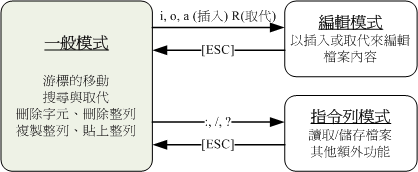
\includegraphics[scale=0.8]{pics/vi-mode} \\

\subsection{Basic knowledge}
\subsubsection{Config a new computer}

\begin{itemize}
		\item What to do if you want to install vim on a new computer?

\begin{enumerate}
		\item Run \linuxcommand{clone https://github.com/VundleVim/Vundle.vim.git ~/.vim/bundle/Vundle.vim}

		\item Go to my github, download my own vimrc and change it to .vimrc. If you use unbuntu, you can download ubuntu\_virmc file and name it to .vimrc
		
		\item go to my github and download vim/ycm\_extra\_conf.py and rename to .vim/.ycm\_extra\_conf.py. YCM will use it. 

		\item go to my github and download vim. Then copy three child directories "after", "plugin" and "macros" to .vim directory.

		\item Open a vim and then run :PluginInstall
		
		\item Go to YCM homepage to see how to intall YCM. In a new version Linux, this can be done very easy.
		
		\item Google how to swap Esc and Cap key. Some OS support swap ESC and Captive, \textbf{I recommend this method.} It's more reliable and just get used to it.
		\item sudo apt-get install xclip . 
		
\end{enumerate}

\end{itemize}

\subsubsection{Basic rules}
\begin{itemize}

		\item \textbf{Rule1: Don't use arrow key any more. At first, you always want to use arrow key to move to right position in insert mode. That is not correct. Any time you want to move, just go back to normal mode, then use "hjkl" and other motion command.}I have disabled arrow key in my .vimrc file.

		\item \textbf{Rule2: Once you go to normal mode, you will have a lot of commands which you combines together to finish your task: 1)basic move, 2)fast move 3)delete+(motion,text objects) 4)visual,copy or move. 5)specific edit(r, surrounds commands) After all necessary task,6)you can use i(I),a(A) o(O) to return back insert mode at right position.}

		\item \textbf{Rule3: I made some mapping in insertmode, but they are just for temporary action to avoid "Esc+one action+i". You should not think that is mainstream operation, just supplement methods. For example, if you want move cursor a lot, first go to normal mode, then use necessary commands,then come back to insert mode. That is better than <Alt+hjkl> in inser mode. If you just want to move one time, please use<Alt+h>.}

		\item \textbf{Rule4: Any time you click same key too many time, stop and google to see if you have better command or smart command, practice until you forget it. }

		\item \textbf{Rule5: But don't overdo it. Don't just focus on trick and plugin. If you can't find solution easily, just give up and focuse on your work, not tool}

		\item  \textbf{Rule6: Most of time, you should be in normal mode,  such as after finish one line, return normal mode and press o go into insert mode again.} 

		\item \textbf{Rule7: c command is more useful than d command, 1)it will go into insertmode directly, 2)and all the action after that can be repeated by . command}

		\item \textbf{Rule8: Any motion support forward and backward directions. Know (ge b * e w) position. Jump short with f or long or special character, such as comma or stop with $\backslash$(fF).}

		\item \textbf{Rule9: Learn to use dot command more, detail can be seen below dot section.}

		\item \textbf{Rule10: Learn to use delete command in insert mode more, such as <C-h,w,u>, del , <c-x>s and <c-t,d>} 
		
\end{itemize}

\subsubsection{Basic knowledges}
\begin{itemize}

		\item Esc is not in good position. You can use <C-$[$> to exit insert mode. You also can map jj to Esc. You also can map <Cap> to Esc. By now, my configuration support these three methods. \textbf{Sometimes, <Cap> will not work, at this time, you should run :!xmodmap -e 'clear lock' command, it will fix this problem.}

		\item In terminal windows, in edit menu, you can see preference. You can "disable All menu access keys", In this way, you can use alt+f or alt+h key in your vim. 
		\item By now, I configure cursor in different shape in insert and normal mode. By adding two command in my vimrc file. For different termnial, there are different solutions, just google it when you get your new computer.
\begin{verbatim}
au VimEnter,InsertLeave * set nocul
au InsertEnter,InsertChange * set cul
\end{verbatim} 		

		\item \linuxcommand{sudo apt-get install vim-gnome}, then use \linuxcommand{vim -g} will support mouse.  With mouse, you can click a position to move there. you also can drag mouse to select a block of text. It's easier to use it.  

		\item :h s will give you detail information about each command. \verb=:h i_CTRL-W= will show a command "CTRL-W" represent in insert mode. "i\_" is insert mode. "v\_" is visual mode. And if you don't use any prefix, it represents all the command in the normal mode. There are two things worth mentioning: 1) Most commands in insert mode is combination key, such as CTRL-?. 2)In the help topic, you can see a lot of other optional insert commands around CTRL-W. You can extend your knowledge by learning other insert commands.

		\item \linuxcommand{vim -v} will open read-only files. You also can use less, but less support doesn't motion command.

		\item \verb=vim -version= will show you a lot if useful information. It will tell you if it support some mode or patch. For example, if you see +quickfix, It means that your vim support quickfix mode. If it shows -quickfix, maybe you need to recompile the whole vim.

		\item .vimrc and .gvimrc are two important configure files, gvim  will read .vimrc first, and then read .gvimrc files.  You can use \verb=if has('gui_running')= to just configure for gvim, not vim in terminal. 

		\item If you run vim in a terminal windows, terminal windows font and size will affect vim.  If you run gvim, You should configure vim font by add to .vimrc files. Detail can be seen in my vimrc file in github.

		\item set LANGUAGE="en\_US.UTF-8" in /etc/rc.conf and LANG="en\_US.UTF-8" in /etc/locale.conf, then logged out and logged back in and it worked. My terminal displays unicode properly now. If don't have root right, set these two varaibles in your .cshrc or .bashrc file.

		\item gvim's color is sharper than vim in terminal.  Maybe it use more colors than terminal.  

		\item g and z don't use as any command in normal mode, so they are prefix as combination command, such as zt,zb, gj, gk, gg. :help z and :help g will show you all the commands that sit behind these prefixes.

		\item \linuxcommand{vim -u NONE} will launch vim without load .vimrc. It will help you if you have some troubles in your .vimrc file or you want to do some experiments. 
				
		\item location list window command: open and close are "lop"and "lcl". For quickfix windows, "cw" and "ccl".
		
		\item Control-operations: C-A, C-X. It will add or subtract some number in normal mode. You need to press number first, then press <C-A>.
\end{itemize}

\subsubsection{Dot}

\begin{itemize}

\item Dot "." is an interesting thing in vim:

		\begin{enumerate}
			\item In normal mode,dot represent repeat last edit command.
						
			\item In register. dot represent last insert content. If you use dot, it will remember a command before you go into the insert mode. If you use ".p, It just paste your insert content at current position. 

			\item In Mark, dot present you last insert position, you can use `dot to jump back, different with gi. gi will go into insert mode.
		\end{enumerate}

\item Below command will be remembered by dot command.
		\begin{enumerate}
				\item insertion : a, A, i, I, o, O

				\item Text changes involving registers: c, C, d, D, p, gp, P, gP, s, S,x, X.

				\item Other text changes: J, gJ, r, gr, R, gR, gU, gu, gw, gq, g?, ~, g~, <, >, =

				\item Equivalent of these operations in visual mode.

		\end{enumerate}

		\item In "practical vim" There are three good examples to illustrate dot command. The first one is tip2, use A add semicolon at the end of each sentence.The second one is tip 3, use s to add two space around +. The third one is tip 5, use cw to replace word. \textbf{They all follow the same routine, One keystroke for motion, and one keystroke for repeat}
		
		\item . just remember the last command in normal mode, so daw is better then two edit command bdw, you can repeat it by dot command later.

		\item  Don't small count if you can repeat. Use count when it matter. Pratical Vim tip 11 give detail explanation. 	

				
\end{itemize}

\section{Text Block}

\subsection{text object}
\begin{itemize}
		\item Common text objects in vim. 
\begin{verbatim}
aw,iw	a word (with white space), innerword		
aW,iW	a WORD (with white space), inner WORD		
as,is	a sentence (with white space), inner sentence
ap,ip	a paragraph (with white space),inner paragraph
	
ab,ib	a () block (with parenthesis),inner () block
aB,iB	a {} block (with braces)	,inner {} block
a[,i[	a [] block (with []), inner [] block

a",i"	a double quoted string (with quotes),inner
a',i'	a single quoted string (with quotes)
a`,i`	a string in backticks (with backticks)

at,it	a <tag> </tag> block (with tags), inner<tag.
a<,i<	a <> block (with <>),inner <> block
\end{verbatim}

		\item There are "a,i" two big categories. There are "w,s,p", "b,B $[$", and "double quote, single quote, backticks". In addtion, There is extra "t,<", Just remember 11 group. You can use them in the "d,c,y,v"commands. Especially you can use "v" command to see if scope of these text objects in your text.  

		\item For text object,  \textbf{delete around, change inside}. Detail can be found in practical vim tip 52. 

		\item \textbf{VimTex} plugin will add new text object, such as vimtex add "e" and "c" two text objects. 

		\item \textbf{Surrord} plugin add another control scope, such as "s" beside "a" and "i".  \textbf{Just remember a", i" and s"}
\end{itemize}

\begin{tabular}{p{0.15\textwidth}|p{0.23\textwidth}|p{0.63\textwidth}}
\hline 
type & text object & surround \\

\hline 
",',`  & (a,i)(",',`) & f"(jump), cs"(, ds" \\

\hline 
\verb=(,{,[= & (a,i)(b,B,$[$) & \%(jump) ds(,cs("  \\

\hline 
<p> head </p> & (a,i)(t,<) & \%(matchit), dst, cst<h1>, 1) phh(Emmet) 2)select,S,<p>(Sround) 3)select,<C-y>,p(Emmet) \\

\hline
/begin ../end & (a,i)(e,c) & \%(matchit), dse, dsc \\

\hline 
w,s,p & (a,i)(w,W,s,p) & Add surrounds: csw", csW", ysiw" yss".  \\

\hline 
\end{tabular}

\section{Basic command}
\subsection{Motion command}
\subsubsection{Move in insert mode}
\begin{itemize}
		\item \textbf{Move in insert mode is not mainstream operation in VIM.}

		\item Move, you should be able to move in both insert mode and normal mode. For some simple move, you should not leave insert mode, that means you can save some time.You need to use \verb!inoremap! to map to alt key, see next item.  

		\item Some consideration about mapping<A-?> in insert mode: (By now, I didn't use it very often, They are history legacy.)
			\begin{enumerate}
					\item All <A-*> need to be use \verb!inoremap <A-t> <C-o>gg! command to map to a command in normal mode. In table, I just keep <A-*>, detail mapping can be seen in my .vimrc file. 

					\item Don't change any command in normal mode, when you use laptop or other computer, when your mapping doesn't work well, you can return to normal mode to use these original commands in normal mode

					\item when you are mapping, you can refer the normal mode, such as <A-w> is move to next word, just like w command in normal mode.

					\item If you just want to have ONE action move or other operation, you don't need to leave insert mode, so mapping the move used command in insert mode, by now, I mapping some move and editing command in insert mode. Detail can be seen in below table.

					\item By now, you can use Alt-char map some commands, and you also can use two captive letter which don't use very often in our language. such as UU RR etc. 

					\item By now, on some computers, if you map alt-(char), It doesn't work very well. Sometimes, when you press it,it will go into the normal mode. I don't have time to investigate right now. 
			\end{enumerate}
\end{itemize}

\subsubsection{Move in normal mode}
	\begin{itemize}

	\item Some basic motion commands: 
	\begin{center}
		\begin{tabular}{p{0.33\textwidth}|p{0.33\textwidth}|p{0.33\textwidth}}
		\hline 
        move position & insert mode & normal mode \\

		\hline
		b/e of document &  <A-f>(begin)  & 1G(or gg) , G  \\

	    \hline 
		b/m/e of screen & <C-o>... & H, M, L \\

		\hline 
		pre/next para & <C-o>... &\{ \} \\

		\hline 
		pre/next sentence & <C-o>.. & $( )$ \\
		
		\hline 
		begin, end of line &<A-i>and <A-a> & (0 or \^{}) and (\$ or g\_)  \\
		
	   	\hline 		
		next, previous word(begin) &<A-w>, <A-b>,<A-e>  & w, b\\   

	    \hline
	    next, previous word(end) & <C-o>.. & e, ge \\
 	
         \hline 		
         match parenthes & <C-o>... & \%   \\
         
         \hline 
		 match next character &<A-q>, <A-z>& fx, Fx, tx, Tx \\
         
        \hline  
		mark and return & <A-m> <A-n> & ma, then `a. \\
        
        \hline 
		return to previous jump position & <C-o>... & <C-o> \\    
      				
		\hline
        search &<C-o>...  & / and ? \\

       \hline       
		previous and next word in cursor & <C-o>.. & \#, * \\

		\hline 
		All /first word in cursor(For C/C++) &  & $[I$, $[i$  \\ 

		\hline 
		will go to next line in wrapped mode. & &  gj and gk \\

		\hline 
\end{tabular}
\end{center} 
		\item \textbf{For left and right two words, and beginning and ending position use w(W) b(B) e(E) ge(gE) command to jump}
						
		\item \textbf{From 2 to 4 words, you can use f and F command to follow a letter. Prefer to use less common character, such as x,j. Avoid aeiou.}

		\item \textbf{More than 4 words, you need to use easyMotion plugin. It also support w(W) b(B) and f command. It will list all options, but you need click more keyboard.}

		\item j k 0 \^{} \$ can add g in front of letter to distinguish real line and display lines.

		\item "f F t T" will not go over multiline. It just search within one line. If you need to multiline search, you can use "/ ?". Or use Easymotion Plugin.

		\item h,j,k,l, w(W), e(E), b(B), \^ , \$ ,fx,tx, (,), \{ ..., gg. All these move command you can add number before them. For example, \verb=4f,= will jump to the fourth ,(comma) directly.    

		\item fx command, then ; and , will repeat forward and backward command, Just like n and N in / and ? Command.

		\item reuse the last search // and last search in sub s//aaaa/gc				

		\item jump lists basic:
\begin{enumerate}
		\item Jump commands are "G","/", "?", "n", "N","\%", "(", ")", "[[", "]]", "{", "}", ":s", ":tag"(When you have tagbar, you don't need run :tag manually), "L", "M", "H"

		\item "w b e j k h l" are not jump command, they will not recored in jump list. "f, F, t, T" are not jump command either.  \textbf{With in one line isn't jump command, You can think it in this way although it's not 100\% accurately.}

		\item When you use easymotion, jump more than one line, it's regarded as jump.

		\item All jump command will record in jump list; :ju will show jump list. Then you can use <C-o> and <C-i> to navigate the jump list. 
		
		\item gi will return last position you exit insert mode.
				
		\item <C-o> will return back last jump positio, <C-\^{}> will switch back to previous file. 

		\item Double single quote and double backtick will toggle current and previous jump. Double backtick will come back exact position. Double single quote will come back previous line position.  \textbf{If you want to jump to one place, then jump back, these two commands are very useful. You don't need use m to mark the original position and use $`$ to jump to mark position.}
\end{enumerate}
\end{itemize}

\subsubsection{Mark}

\begin{itemize}

		\item marks lists basic:
		\begin{enumerate}
				\item :marks command will show you all the marks list. 

				\item Basic command is ma and 'a. 

				\item Low case letter just mark position in current file. Captive letter can mark a position in different file, when you jump to this position, you don't need to open this file manually.

				\item There are single quote command, backtick command. Single quote will jump to exact mark, backtick will jump to mark line. They need follow a mark name.

				\item \`{}. will return your last edited position.  \`{}" will return exit position of current buffer. And \`{}0 will return exit position of file(when vim exit, That is to say, The last file you are working when you exit your vim last time.) 

				\item Double single quote command will help you to jump back origin position, but still in normal mode, \textbf{gi command will return back to the position where you exit insert mode, and return back to insert mode. It's very useful command. }
				
\end{enumerate}
\end{itemize}
\subsubsection{Search}

\begin{itemize}
\item search command in VIM:
		\begin{enumerate}
				\item \linuxcommand{:lv word \%} will search all word in current file. It will show all the result in position list. 

				\item position list is associated with current window, and quickfix list is global.

				\item You can use :lne :lw :lpr to manipuate position list windows. You can use :cne :cw :cpr to manipuate quickfix windows. 

				\item If you want to find all key words in the current file, you can use :lv. If you want to find all words in the multi files in one project, such as a C++ project, you can use $\backslash$vv command, It's vim plugin. It will show all your result in quickfix window. 

				\item You can use \# and * command, you don't need to input word which you want to search. 

				\item If you use / or ?, you can use <C-r> <C-w> to paste current word to command windows. or you can input manually. 

				\item \textbf{Press F4 to toggle highlight research result.} 

		\end{enumerate}
\item regex in search command:
		\begin{enumerate}
				\item vimgrep use // to enclose pattern, but when you use / it's a little different, /abc/e search abc and put cursor to end.

				\item patten example 1) escape html 2) search duplicate word. 

				\item $\backslash$v magic; $\backslash$c case incentive

				\item There are two subtopics, One is regex syntax is different between grep, python and vim. The detail can be see below link.  https://remram44.github.io/regex-cheatsheet/regex.html\#syntax-basics And a good regex example can be found here:  http://www.rexegg.com/regex-quickstart.html
		\end{enumerate}

\item Three methods search: 1)"/,?" 2):lv 3) easygrep plugin
		\begin{enumerate}
						\item / search current buffer, it support regex too, but it will not output result to position list or error list. 

						\item :vim(grep) and :lv(imgrep) difference lies in write to location list or quickfix list.

						\item :lv need follow \% to represent the current file, or *.c which means all c file. Or you ca use **$\backslash$*.c which means recursive. But a better way is using easygrep plugin. You only need $\backslash$vv command.
										
						\item $\backslash$vv is just syntax sugar of :vimgrep. You don't need input word manually, and it will open quickfix window directly. The shortcoming is you can't edit regex manually. 

						\item You can use :GrepOptions to turn on recursive, so vv will find all .h or .c or .cpp files.
								
						\item For :lv,You can input complex regex manually, So :lv is more flexible than $\backslash$vv. $\backslash$vv is more convenient than :lv. 
						\end{enumerate}

		\item :marks :ju :reg :change are three useful commands. 		
\end{itemize}

\subsection{Edit command}

\begin{itemize}
\item Below are some edit commands:
\begin{center}
		\begin{tabular}{p{0.33\textwidth}|p{0.33\textwidth}|p{0.33\textwidth}}
		\hline
		delete & insert mode & normal mode\\

   	    \hline 
		delete previous character & backspace,<C-h> & hx(move then x) or X  \\
	
		\hline 
		delete and replace current character & <A-x> & x , s , r\{char\}  \\
	
		\hline 
		delete word to end & <A-c> & (d,c)e or w  \\
		
		\hline 
		delete word to begin & <C-w> &(d,c)b or ge  \\

		\hline 
		delete current word &<A-b>,then <A-c> & daw or daW \\
		
		\hline 
		delete line to end & <A-v> & D or C  \\
		
		\hline 
		delete line to begin & <C-u> & d\^{} or c\^{}  \\
		
		\hline 
		delete current line & <A-d> & dd S cc \\

       \hline
	   replace in current line &<C-o>.. & :s/old/new/g(c) \\

		\hline 
	   replace in whole file &<C-o>.. & :\%s/old/new/g(c) \\

	   \hline
		indent and unindent & <C-t> <C-d> & >> and << \\

	   \hline 
	   Join next line & <C-o>.. & J \\ 

	   \hline 
		swap line with next &<C-o>.. & ddp \\
	
		\hline 
		undo and redo & <A-g> &  u and . (ctrl+r) \\ 
		
				\end{tabular}
	\end{center}

\item tricks about edit command: 
		\begin{enumerate} 
				\item  Edit commands "d,c,y", \textbf{d keep in the normal mode. c go to insert mode. y keep contents.} 

				\item \textbf{d,c,y can all follow EasyMotion command.}

				\item C delete to the end of line, and go into insert mode. D is the same, but stay in the normal mode. S delete the whole line, and then go into the insert mode. X delete previous character. \textbf{remember(s,x), (C,D) and (S,dd).}
						
				\item d c y > < = g~ gu gU are operator, They can follow motion, and operator+conquer.

				\item All previous operator can follow motion, it give edit command a "operator scope". For example, "d2w" will delete next two words. "d3j" will delete next 3 lines. "ct;" will delete every thing until ";", it's very useful for C++ language. 

				\item  At the same time, all operator also can follow text object, such as "aw" and "iw". A list of text objects can be see below.  You can use \verb=di"= to delete all the contents inside of a pair of double quotes. You also can use \verb=da"= to delete all the contents plus a pair of double quotes.There are 11 groups common used text objects which I introduced in previous section. 


				\item 3dd and 2dw   \& support number+command means how many times you will perform this command.

				\item <C-h> <C-w> <C-u> and del, these four commands can delete in insert mode. Learn to use <C-h> more, It's easier than type backspace.
					
				\item <C-r> and <C-r>= paste in the insert mode.

				\item After select, use c to delete and into insert mode.

				\item x stay in normal mode, s go into insert mode, r need to follow a letter and stay in normal mode too.
						
				\item \textbf{c is same as d, and s is same as x, but they will go to insert mode, you should use them more, to avoid use i, a later.}  
				
				\item command v also can follow motion and text objects. It can give me a tip. If you are not sure what you will delete, you can use v command to highlight, if highlight is not what you expect, you can Esc, and adjust you motion or text object, until you get what you expect. 

				\item ggyG will select all contents in a file. such as Ctrl+A and Ctrl+C 

			\item "ddp" swap lines. In fact, it is two commands, "dd" and "p". If you understand it. you can know "xp" is swap character. And "dawwP" is swaping word.

			\item "J" can be use to delete empty line below.

			\item \textbf{When you use delete to a character at long distance, You can use d$backslash$[fF] to give exact position, Or you can use df, than use dot command to repeat it. }
	\end{enumerate}
\end{itemize}


\subsection{Scroll}
\begin{itemize}
\item scroll command, scroll window, but cursor will stay in the same position.
\begin{center}
 \begin{tabular}{p{0.33\textwidth}|p{0.33\textwidth}|p{0.33\textwidth}}
        \hline
        scroll one  page &  <A-t> and <A-y>  & ctrl+b and  ctrl+f    \\
        
        \hline 		  
        scroll one line &  <A-u> and <A-r>  & ctrl+e and ctrl+y \\
        
         \hline 		  
        move cursor to m/t/b & <C-o>...    & zz zt zb \\
		\hline
    \end{tabular}
\end{center}
\item \textbf{zz command use more often when you want see more.}
\item \textbf{Don't use j,k command to see more content(turn page, or scroll).}
\end{itemize} 

\subsection{Window}

\begin{itemize}
		\item Control windows commands:

\begin{center}
   \begin{tabular}{c|c|c}
   \hline
		move & insert mode & normal mode \\
		
\hline 
		switch window & <C-c> &  Ctrl + w\{h,j,k,l\}\\
				
		\hline 
		split window & <C-o>,then :sp  &  Ctrl + ws\\
		
		\hline 
		close a window & & Ctrl + wq or <C-x>\\
		
		\hline 
		close all other & & <C-w> o \\

		\hline
		split window vertically	&   & :vsp \\ 

		\hline
		window resize	& &  <C-w> [count]+,- \\ 

		\hline
		window vertical resize	& &  <C-w> [count]<,> \\ 
		
\hline 
			\end{tabular}
	\end{center}

\item <C-w>,o is more useful when you want to close other windows, You don't need switch to another windows.
\end{itemize}
	
\subsection{Buffer}
\begin{itemize}
		\item Manage buffer:
\begin{center}
\begin{tabular}{p{0.33\textwidth}|p{0.2\textwidth}|p{0.33\textwidth}}
		   \hline
		Action & insert mode & normal mode \\
		
		\hline 
		edit a file in a new buffer & &  :e file\\
				
		\hline 
		next, previous buffer & RR &  :bn :bp , <C-\^{}> \\
		
        \hline 
		go to number buffer &<C-o>.. &  :b num \\		
		
		\hline 
		delete a buffer & & :bd \\
		
		\hline 
		list all open buffers & & :ls\\
		
		\hline
		open a file in a new buffer and split window
	 & <C-o>..& :sp file or :vsp file \\
	\hline 	
			\end{tabular}
	\end{center}

			\item Closing windows is different with deleting buffer. When you use :bd command. It will close the windows too. If you want to just close buffer. You should use :bn to switch to another buffer, then use :ls to know the buffe number which you want to close, in the end. use :bd num close to close it background without close current windows.

		\item use :ls! command will show all the buffers. Such as Nerdtree buffer, VimtexToc buffer. To reload buffer into certain windows. 

			\item \texttt{:bd} will close current buffer, you can follow number to close specific buffer. You also can use \texttt{:bd+space+tab} will list all the avaible buffers.

			\item Any time you want to switch buffer or open new buffer, save current buffer first.
			
			\item ":e" will open buffer in current window. If you want to open in a different window, you can use "sp file" or "vsp file".

			\item Open another buffer in splite window, \texttt{:sp | b1} Pay attention, it's different with :sp file-name.

			\item Usefule commands:
				\begin{enumerate}
					\item Open at current windows, 1):e file 2) <C-n> seletct file and enter. 

					\item Open at split windows, 1):sp file 2) <C-n> select file and i

					\item Open at vsplit windows 1):vsp file 2) <C-n> slect file and s

					\item For CtrlP plugin, <C-p>, then <C-o>, you can select which window to open.
				\end{enumerate}
	\end{itemize}

\subsection{Visual}
\begin{itemize} 
		\item Basic commands are below:
		\begin{center}
				\begin{tabular}{c|c}
						\hline
						v, V, Ctrl-v  & being select\\

						\hline 
						d, y & copy and delete\\

						\hline
						<,> & indent left,right\\

						\hline
						V, yy & select, copy the whole line  \\

						\hline
						gv & reselect previous select \\
						
						\hline 
						o & toggle free end of selection \\

						\hline 		
				\end{tabular}
		\end{center}

	\begin{enumerate}
			\item Using v to exit select mode is faster than Esc. 

			\item o command change free end, make you can select text more freely.

			\item \textbf{Almost all the motion commands can be used in visual mode.}

			\item \textbf{You also can use EasyMotion command in visual mode.}
					
			\item <,> will exit select mode, gv will select it again. 

			\item . can repeat visual edit command.But it act on the previous selected region.  
					
			\item \textbf{prefer operator+motion than visual, because it can repeat.}
	\end{enumerate}					

	\end{itemize}

\subsection{Register}
	\begin{itemize}
			\item You can check all register by :reg command 
			
			\item gP is useful when you want to paste multi-line text several times. See "Practical VIM tip 62". Captive P and gP can be used in this contidtion. When you use "g", The curser is near orignal one. When no "g", the cursor is near copied region. That's all.

			\item :reg will show your list of register."0 will always have the content of the latest yank, and the others will have last 9 deleted text, being "1 the newest, and "9 the oldest.

			\item " will change when y and delete, and 0 will save y. and 1~9 save large block delete. 

			\item Default register is ", so p command is equal ""p .

			\item \textbf{". save all your content that you just insert.} So if you want to repeat some line, first, you can insert, then use ".p . Then in the end, use . to repeat previous command. 

			\item "ay will copy some thing to "a" register, "ap will paste it.
					
			\item "Ay will appnd something to "a" register.

			\item Unnamed register, yank register,  named register(a-z) expression register, only read register "\% \# . : /" five registers. 

			\item paste from register,  include character-wise and line-wise 
					
		\item In Vim, there are three clips: 
				\begin{enumerate}
						\item \textbf{Basically, there are three different method to paste, 1) vim register 2) normal clip, 3) xclip} 

						\item normal clip, You only can use mouse to select(It will add line number into your selection), then in insert mode, right-click mouse to popup menu, select paste; Or shift+insert. \textbf{Don't use Ctrl+C and Ctrl+v, and must do it in insert mode, or all you content will be input as command in the normal mode, It's dangerous}

						\item xclip, Use mouse middle-button to past in Vim.\textbf{Must in insert mode, and It's not good method.} When you use xclip, you should click left mouse first, then click shift key. When you finish select, it will go to xclip, then you can use F7 to paste in VIM in normal mode, it will keep format. 

						\item vim own clip, use y and p command. \textbf{Must in normal mode}

						\item The contents of a register can be pasted while in insert mode: type Ctrl-r then a character that identifies the register. For example, Ctrl-r then " pastes from the default register

						\item Use \linuxcommand{vim --version} to see if vim has been compiled with clipboard, If there is + symbol before it. You can use "+y and "+p to copy and past selection to system clipboard. If not, Just use mouse middle-button.
								
						\item Sometimes, when you copy source code from browsers, then use shift+insert to paste it, The format will be messed. You should use shift+mouse to select and copy content to xclip. Then in your vim, 1) move your cursor to insert position, 2) in normal mode run \verb=:r!xclip -o<CR>=, it will paste according to right format. Don't use normal clip and xclip in insert mode.

						\item Add key map to .vimrc, detail can be found in .vimrc file.By now, I map it to F6 and F7.  \end{enumerate}
\end{itemize}

\subsection{Format}
\begin{itemize}
	\item format command : Other reformat tricks can be found in next section "Programmer tips" 
 \begin{center}
        \begin{tabular}{c|c}
		\hline 
		=, =\% & format, format\verb={..}=\\

		\hline
		== & format current line \\ 
		\hline 
		15G=25G & will reformat from 15 to 25 lines
		
	\end{tabular}
	\end{center}
\end{itemize}

\subsection{Ins-completion}
\begin{itemize}
		\item Basic help information can be seen in :h ins-completion. 

		\item In order to reduce number of options, you should input two or three letters firstly.

		\item Ctrl-n,p will navigate all the items in the pop-up menu and accept it. Up and down just navigate. And Ctrl-e close pop-up menu, and Ctrl-y accept the current item. 

		\item Ctrl-x, Ctrl-k will finish word by dictionary. 

		\item Ctrl-p, Ctrl-n will finish word previous and next part. It's useful for programming. Usually, Ctrl-p will pop up previous options, they are very useful in programming because you don't need remember previous long variable name. 

		\item Ctrl-x, Ctrl-l will finish previous line. It will list all previous lines first. 

		\item Ctrl-x, Ctrl-f will finish file name. 

		\item Ctrl-x, Ctrl-i insert keywords in current and included file,  Ctrl-] will insert tags, You need produce a tag file. Ctrl-d will insert definitions or macros. They are very useful for C/C++ and python programming.

		\item :set spell , then $[$s, then , zg it's right word, zu is not right word

		\item In insert mode, <C-x>s will jump back to the first error word, and pop up spell correction windows. 
\end{itemize}

\subsection{Ex command}
\begin{itemize}
		\item \textbf{tab also can help you finish when you type :command.}
				
		\item ex command strike far and wide
		
		\item  For ex command, ".", "\$", "\%" , "'<"  and "'>" represent different [range], "." is current line, and "\$" is the last line of the file. and "\%" is the whole file.
		
		\item \textbf{:\%normal i//} while file, perform a normal mode command, Here is insert // . 

		\item @: repeat last ex command.
		
		\item :shell will open shell window, you can run some shell command, then input exit to close shell window. 
		
		\item q: will open command-line window, :quit will close it. Sometime, when you want to use :q, but you misstype q:, You will go to the command history windows, At this time, you only can use :quit to quit this windows, or press enter on an empty line.
\end{itemize}

\section{Plug in}

\subsection{Vundle}
\begin{itemize}
		\item About vundle usage, I have added a bookmark to evernote. First you need run "git clone https://github.com/VundleVim/Vundle.vim.git ~/.vim/bundle/Vundle.vim", then just need to edit .vimrc file.  

		\item When you have vundle installed, you can edit .vimrc to install others plugin. By now, I have backup my .vimrc file. When you transfer to other computer, you can use it directly. 

		\item You can google "vim awesome". It introduce a lot of vim plugins. By now, what I installed can be found in .vimrc file. You can download my .vimrc from my github new\_doc repositor.
		\end{itemize}

\subsection{Appearence}
\subsubsection{Solarized}
\begin{itemize}
	\item vim-colors-solarized, it can be only used in vim in terminal, It only support 16 color. You need to go to  vim "color scheme test c website" (add it evernote) and select you favorite scheme. and then download it. put it in .vim/bundle/vim-colors-solarized/colors directory. Then you can modify your .vimrc.
	
\begin{verbatim}
if has('gui_running')
colorscheme blacklight
else
colorscheme solarized
endif 
\end{verbatim}
	\item When you use solarized plug in(theme), you have to change the terminal. For some new version gnome terminal, you can see terminal->preferences->profiles->color tab, there is solarized dark option in "text and backgroud color", and solarized option in "build in scheme in palette", just select it.

    \item When you have old terminal, There are two options, for some old gnome terminal, there are no import color option, you can download Anthony25/gnome-terminal-colors-solarized in a temp directory, and then come to this directory and run .install. You need to first add an solarized profile, then the application will ask if which profile you like to overwrite, select solarized profile, you can keep you original default unmodified. Then you can select your solarized profile, the color will be set properly. 

\item If some keyword highlight background color is not correct, you need add \verb!set t_Co=16! to your .vimrc. 

\item For mac, you can download tomislav/osx-terminal.app-colors-solarized(I haven't tried it yet). Or you can download git:altercation/solarized. There is directory \verb!osx-terminal.app-colors-solarized/!, you can import *.termnial file in your mac terminal preference color. That is all.
\end{itemize}

\subsubsection{vim-airline} 
\begin{itemize}

\item You can go to "https://github.com/powerline/fonts" download font package. Then extract it. Go into the directory, then run ./install.py.  All the font will be installed in HOME/.local/share/fonts. Then you go to your HOME directory. Build a link. "ln -s HOME/.local/share/fonts .fonts". Then you gnome-terminal preference window will show Powerline fonts. Select "Literation Mono Powerline". Building link is very important step for gnome-terminal. 

\begin{verbatim}
if has('gui_running')
set guifont=Literation\ Mono\ Powerline\ 12   
let g:airline_powerline_fonts = 1
endif
\end{verbatim} 
\end{itemize}

\subsection{File explorer}
\subsubsection{NerdTree}
\begin{itemize}
		
		\item \textbf{Use ctrl+N to toggle nerdtree window}, then Ctrl+C change window, once you are in nerdtree window, you can use all motion command in normal mode to move your cursor. You also can change to visual mode and use 'y' to copy a file name and paste it back to your main editor file.  

		\item \textbf{shift+i will show or hide hidden file.}

		\item When in the NERDTree window, press 'm'; you should see a menu at the bottom. Type in 'a' for add childnode. Now input the directory you want to create, making sure to add a '/' at the end, otherwise the script would create a file.

		\item In the NERDTree window, you can press 'm' and 'l', then you will get whole directory informaiton. Then you can use mouse to copy it and paste it back to your main edited file.

		\item When you are in the Nerd window, you can press Enter to open in current windows. "s" will open in vsplit window, "i" will open in a split window, If you forget, press "?" to toggle to show all the useful commands.

		\item For some very deep file, you can use :Bookmark bm. Then "B" will show all the Bookmark table. Then you can navigate Bookmark table to open a bookmark file.

		\item You can use "u" to jump up one level in directory tree. Or use "C" to change current directory as tree root."r" will refresh the directory.

		\item By now, preview will open a new buffer inside vim. So this feature is not what it really like. There are some solutions, but I don't want to try them right now.

		\item use p to jump to parent folder position, and .. go up level
\end{itemize}

\subsubsection{Ctrlp}
\begin{itemize}
\item use ctrl+p to invoke ctrlp plugin, Don't use :CtrlP command  \\ 
\begin{tabular}{|p{0.25\textwidth}|p{0.75\textwidth}|}
\hline 
ctrl+f,b  & cycle between modes \\ 

\hline 
ctrl+r & switch regex mode  \\ 

\hline 
ctrl+d & switch to filename search instead of full path \\ 

\hline 
ctrl+o, t or x & open, open file in new tab or in new split \\ 

\hline 
ctrl+z  & mark and unmark files \\ 

\hline 
\end{tabular} 
\item CtrlP will open "current working directory" in vim. You can use :cd directory to change "working directory". You also can input .. to go up parent directory. Default, CtrlP also look for .git as a flag of "Whole project". You can custom your favorite setting according to your context.

\item CtrlP also provide "most recent files" function.

\item \textbf{With Ctrlp and NerdTree, vim has powerful tool to deal with files and directory. You can navigate file system structure by Nerd, add mark by Nerd, or search them quick by CtrlP}
\end{itemize}

\subsection{Motion}
\subsubsection{Easy motion}
\begin{itemize}
		\item Jump to word, use <leader><leader>w,b,W,B,e,E,ge,gE. 

		\item For multi-line, use <leader><leader>j,k.  

		\item :help easymotion.txt give you detail information.

		\item \textbf{f command is very very usefule!}.So I map it just one <leader> before f command. 

		\item If you want to jump to long distance, <leader>f is your best friend. 

		\item You also can try <leader><leader>n,N command, it will repeat you last / command and give each match a tag.

		\item "<leader><leader>."  will repeat the you easy motion command. 

		\item \textbf{By now, I map f and F to single <leader>,And by now, It support d and c command}.
\end{itemize}

\subsubsection{Match it}
\begin{itemize}
		\item It's old plugin, so maybe it will not work very well, Don't expect it too much.
		\item It support <p> </p> jump and /begin /end jump.

		\item It don't need if..else if.... jump. But you can build .vim/after/plugin/c.vim and cpp.vim. and add below to it. And it will support if..else if... else jump and switch...case. default. jump

		\item g\% will jump backward. 
\begin{verbatim}
let b:match_words= '\%(\<else\s\+\)\@<!\<if\>:\<else\s\+if\>:\<else\%(\s\+if\)\@!\>,' . '\<switch\>:\<case\>:\<default\>'
\end{verbatim}

	\item There is another python matchit plugin. It support for(while)...break(continue). if..elif..else, and try..except..finally jump.   
\end{itemize}

\subsection{Surround}
\subsubsection{Surround}
\begin{itemize}
		\item There are three main actions. delete(ds), change(cs) or add surrounds(ys)

		\item When you use delete or change, you should put your cursor inside a pair of surrounds.\\

		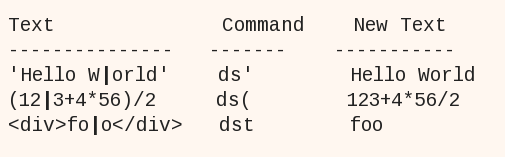
\includegraphics[scale=0.4]{pics/surround1.png} \\

	\item below is change command list: \\

	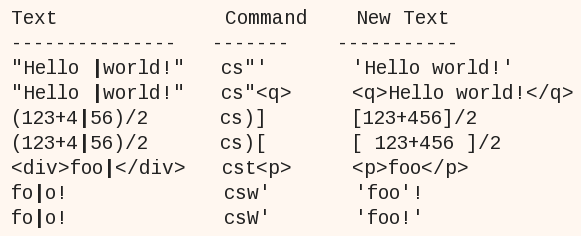
\includegraphics[scale=0.4]{pics/surround2.png} \\
		
		\item Surroundings can be added with the same "cs" command, which takes a surrounding target, or with the "ys" command that takes a valid vim motion. \\

			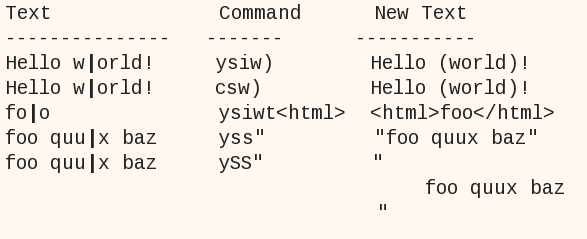
\includegraphics[scale=0.4]{pics/surround3.png} \\
	   
	   \item You can use csw" or ysiw" to add surrounds. ys can follow a valid vim motion. Such as ys3w<p> will add <p>word1 word2 word3</p>
	   \item ys follow 1) text object, 2) f 3) ss.
			   \begin{enumerate}
						\item ysiw" is different with ysw". ysw" will just add " in the exact cursor position, but ysiw" will add " around word which cursor is in. 

						\item ysf;) will add () around before ";".

						\item For a single line. You can use yss command. It's better than Emmet. In Emmet, you have to visual select this line first.  
								
						\item \textbf{If you want to add surrounds to random scope, You can use visual mode, with some easy-motion command to select a scope, after it, you can use "S" to add surround}
						\item \textbf{By now, EasyMotion support single <Leader>, so you can use ys$\backslash$f<ch><ta>" to add " around scope, it's quicker.}
				\end{enumerate}
	   \item In Visual mode, press <S-s> (captive S). Then input a surround that you want to add. Don't use lower case "s". 

	   \item You need install repeat plugin too. For example: there is text "<p1><p2>word</p2><p1>". You put cursor inside word. Then you can use dst. Then press . It will delete pair of <p1> and <P2>. repeat plugin just for Surroun plugin. 
	    
	    \item Surrounds are useful for edit html doc. It's overlap with Emmet. For example. In visual mode. \verb=<C-y>,= will trigger expand mode in Emmet. Then input <h1>. Or you can use <S-s>, then input <h1>. It will add a pair of <h1> 
\end{itemize}

\subsubsection{Repeat}
\begin{itemize}
		\item . only repeat edit command in norm mode. And only for these native edit command. It will not repeat move command

		\item move command are most single character, So I don't need to use . to repeat it. If you like, there is plugin for it. 

		\item For some customized edit command, such as Surrounds below. native . command will not support it. So, I need to repeat vim plugin installed. 
\end{itemize}

\subsection{Html and text}

\subsubsection{Vimtex}
\begin{itemize}
		\item Vimtex is lightweight plugin for Vim. I didn't use compile ability right now. 
				
		\item Vim tex provide another text objects. Such as "ae ie", "ac ic" and "ad id". 
				
		\item By now, I map F3 to :VimtexTocToggle.This is most useful feature which I used. 
				
		\item ]] in insert mode finish environment automatically.
				
		\item [[ ]] command navigate by section.
				
		\item (cd)*(se sc sd) six commands. 
\begin{verbatim}
1)\begin{aaabbb}
ac is "\begin{aaabbb}"
ic is "begin"
dsc will delete "\begin{}", aaabbb is left.

ae is whole enviroment
ie is inside enviroment
dse will delete "\begin{}" and "\end{}" 
\end{verbatim}
	\item By now, I don't delimiter, it used mainly for math equation. So I don't use "ad id" and "dsd" very often. 
\end{itemize}

\subsubsection{Emmet}
\begin{itemize}
		\item <C-y>, is trigger key in Emmet. I map "hh" to expand abbreviation.

		\item Below is simple table, detail can be google by"emmet abbreviations syntax". Abbreviation is the most important topic in Emmet. Besides, it, It provide other useful command.  For practical usage, you still need to come back to look at its tutorial. \\

\begin{tabular}{p{0.25\textwidth}|p{0.75\textwidth}}
\hline 
html:5  & whole page \\ 
\hline 
>,+,\^{} & child,sidling, parent  \\ 
\hline 
* &how many times output \\
\hline
div\#id, div.class & with id and class to a tag \\

\hline 
\$ & will attach number with elemental attribute name   \\

\hline
text \{ \} & add text to element \\
\hline
\end{tabular}

\item An example, type \verb=div>p#foo$*3>a=, The <C-y>, 
 <div>
       <p id="foo1">
		   <a href=""></a>
	   </p>
	   <p id="foo2">
		   <a href=""></a>
	   </p>
	   <p id="foo3">
		   <a href=""></a>
	   </p>
</div>

\item Some directly edit commands. \\

\begin{tabular}{p{0.25\textwidth}|p{0.75\textwidth}}
\hline 
<c-y>+k  & remove a Tags pair and content inside \\

\hline 
<c-y>+d,D & Balance tag outward and inward  \\

\hline 
<c-y>+a & move to URL, add anchor to it \\

\hline
<c-y>+/ & toggle comment \\

\hline 
<c-y>+i & In image tag, refresh image \\

\hline
ctrl+n,N & move to next available position \\
\hline 
\end{tabular}

\item This tutorial is very simple, website give you detail examples, you can learn it when you work on html pages. 

\item You can type p, then type hh, It will expand <p></p> and insert cursor will be in the middle. 

\item For some exist test, first select, then type <C-y>,, It will move curser to bottom to wait for you input tag.You just need input "h1", don't need to input "<h1>". Emmet will add < > for you automaticlly. If you use surrounding, select, and shift-s. input "<h1>". 

\end{itemize}

\section{Programmer tips}
\subsection{Basic}
\begin{itemize}
		\item Build a IDE-like Vim, You need below plugins:
		\begin{enumerate}
				\item File explore: NerdTree and CtrlP.

				\item Tag jump: tagbar, cscope and easyGrep, gD command and Ctrl+](need tags file), Ctrl+t return.

				\item Error jump: quickfix.

				\item Syntax: syntactic plugin(For python and C++, YCM will use Syntax show syntactic errors)

				\item Autocomplete: SuperTab, Vim-snippet, YCM, Ctrl+p.

				\item Debug: pyclewn.

				\item Comment: Nerdcomment.

				\item Fold: For C/C++, just :set foldmethod=syntax, For python language, use simplyFold plugin 
		\end{enumerate}

	\item For some large scale C/C++ projects, There are a lot of source code which are in a deep directory structure. You can use below tips:

\begin{enumerate}
		\item \linuxcommand{find . -name "*.c" -o -name "*.cpp" | xargs git add} to add all source code files to git, Then you can build a branch test. You can apply this methods to all .cxx and .hpp and .h files. 
				
		\item For ctags and cscope and doxgen, \textbf{you can download my project template cmake-test from github. There are src-tool.sh in src directory, you can use them automatically.}

		\item Use :set path, then you can jump to header file by "gf" command, then use <C-\^{}> to return. A more useful command is <C-w>f command, it will open header file in a new windows.  

		\item First, you need to use Nerdtree to get all directory information, Then set path+=<paste directory here>. In the end, you can use gf command to open header file.

		\item Use F8 to open tagbar windows, it shows all global variable and function in this files.

		\item If you want to search withing specific directory, you can use easyGrep tool. Detail can be seen esayGrep section.
\end{enumerate}

		\item :set number; syntax on and set ai;  Whenever you hit Enter to start typing on the next line, vim automatically will indent to the same amount as the previous line.

		\item Python indent show plugin is <leader>ig. You can change its color if you dislike default configuration. 				
		\item Why jumping to brace is so important? First, use previous commands to jump to open brace. Then \verb!=\%! will format the matched scope. \verb=v\%= will select the whole scope.  After you select, you can input = command to reformat.  

		\item Reformat will perform action according to the previous lines indents. So before reformat, you can use == reformat the previous line of code to right indent.
 	
	 \item ctrl+v will invoke visual-block, you can decrease indent of block or delete a block of comments. 
	 \begin{enumerate}
			 \item ctrl+v, then select block of comment source code 
			 \item don't press Esc, press I (capital i) 
			 \item input // 
			 \item press Esc, then, all the block will be commented.
			 \item A better method is to use Nerdcomment.
	 \end{enumerate}
\end{itemize}

\subsection{Fold}
\begin{itemize}

		\item For fold C/C++ correctly, write big bracket after class, function and if.. statement, and put it next line the first column, in this way, you can use $[[$ command to jump to the fucntion beginning quickly. I didn't use fold very often. 

		\item In vim ,there are different fold methods, and you can't combine them together.  The most useful Syntax, And if you want to use zf command, you have to change it to "manual" method. 
				
		\item fold commands are below, they are VIM commands, not plugin command.
		\item Just remember three common commands za, zo and zc. 

\begin{tabular}{|c|c|}
\hline 
\textbf{key} & \textbf{action} \\ 
\hline 
za, zo, zc & toggle, open, close \\ 
\hline 
zj,zk  & jump to previous and next fold\\ 
\hline
zM, zR & Close , Open all \\
\hline 
$[$z, $]$z & move to the start,end fold \\
\hline 
zf\string & fold to string \\
\hline 
 \end{tabular} 

\end{itemize}

\subsection{Syntastic}
\begin{itemize}
		\item :Errors to open error windows. 

		\item Everytime when you save file, syntax error will listed on left side.

		\item You can use :lne to jump to next Syntastic error, use :lclose to close Errors windows. They don't show on the quickfix window. 
				
		\item There are two checker for latex, one is chktex, you can download and install it from source code. The other is lacheck. lacheck will not ignore text in lstlising enviorment, and it will report a lot of errors. It's annoying. chetex can ignore content in lstlisting enviorment.

		\item You can goto tex document directory, you can build a .chktexrc file and add below to it. 
\begin{verbatim}
CmdLine{
--nowarn 1
}

VerbEnvir{  verbatim comment listing verbatimtab rawhtml errexam picture texdraw
  filecontents pgfpicture tikzpicture minted
}
\end{verbatim} 

		\item For Syntax error use :Errors, it open location list.  For compile error, use quickfix mode, It use quickfix window.   nowarn use to suppress some unnessary warning message.
				
		\item You can add \verb!let g:syntastic_tex_checkers=['chktex']! to tell Syntastic use chktex to check latex.

		\item For latex document, there are a lot of unimportant error, You need to supress them. When you use lacheck, you can't suppress warning. But you can add tex.vim file to after/ftplugin to deal with some tex type file. In this file, you can add let g:syntastic\_quiet\_messages to it, detail can be seen this file.

		\item chktex doesn't check unmatch big brace, but lacheck will not ignore lstlisting env. \textbf{So, They are not good tool for latex check, just a refence, not perfect at all, Don't spend time on them}.

		\item default use chktex, after write, jump to Errors windows and search "error", If there is no error, You can use lachek in you command line to look for unmatch brace error if you document doesn't have lstlisting env. That is all.

		\item \textbf{For Cpp latex document, use chktex, in other document, use lacheck and don't use lstlisting enviroment}

		\item For python language, you need to install flake8. You can use \linuxcommand{pip install --user flake8} to install it. It will install it in ./local/bin directory. You don't need configure Syntastic plugin, default it use flake8.

		\item For html language, You need install tidy, By now, I download it from github and use cmake to build it. detail can be found in build document. 

		\item My web use a lot php file. So You need to add this line to .vimrc. So when you edit .php file, when you save it. It will use tidy to check all the html content in php file.
\begin{verbatim}
let g:syntastic_filetype_map = { "php": "html" }
\end{verbatim}

		\item :SyntasticInfo will show some helpful informaiton, when syntastic doesn't work, you can run this command to see some detail. 

		\item For C/C++ language, Syntastic use clang to check errors in C/C++ language. If you use YCM, It will trigger syntastic check automaticlly.

		\item If you instal YCM, for cpp file, :Errors will not work anymore. When you reach error line, error message will be shown in the bottom automatically. 

\end{itemize}

\subsection{Code navigation}
\begin{itemize}
	\item gD, go to the func or variable defination. It's just jump the first appearance in the current file. It has no any semantic. Another otpion is Ctrl+], it's just like :tag command. It will need you have tags file produced by ctags command. For example, you can use ctags a.cpp to produce tags file, then in you vim, you can use Ctrl+]. The problem is by now, ctags doesn't produce local varaible inside a function.  This problem can be resolved by easyGrep partly.

	\item  Program motion:
\begin{enumerate}
 	\item C/C++ jump bracket:
%\begin{lstlisting}[frame=single, language=c++]
\begin{verbatim}
fun()
{"[["
   ...
}"[]"

main()
{"[["
   {"2[{"
	 {"[{" 
	   {"?{"
	   }
	   {"F{"     } *
}
{"]["
.....
}"]]"
%\end{lstlisting}
\end{verbatim}

\begin{enumerate}
		\item * is your position
		\item \verb=[[,[],][,]]= First is directory, second is opening or closing brace. They just jump to the first column
		\item Find match open brace, you should use f/F or /or? command. 
		\item \verb=[{ or ]}= will jump unmatch braces. 
		\item \verb=[( or ])= has same usage.

		\item The above four commands can be used to go to the start or end of the current code block.  It is like doing "\%" on the '(', ')', '{' or '}' at the other end of the code block, but you can do this from anywhere in the code block.
\end{enumerate}

\item \% can be used jump brace, with Matchit, You can use it jump if else in C and try except in python. You need to another file to support it, detail can be found MatchIt section. 

\item Visual Mark is also a good plug in, usage is very simple, mm visual mark, F2 and shift F2 navigate.

\item Tagbar support python and C at the same time. Cscope only support C/C++.

\item EasyGrep is also a good plugin, detail can be found in below plugin part. 1) Just like cscope, it can be used for python file and produce a list reference position, 2) It support replace mode, and it's very helpful for refactory.

\end{enumerate}

\item \textbf{Tagbar give yo global scope function name and variable, but It will not give you local variable. It support C/C++ and python file}

\item \textbf{easyGrep only support multi file search, If you need local file, you can use :lvim, It will show a list result in location window, you can use :lopen, :lne, :lpr, :lclose command}

\item \textbf{cscope support a little syntastic analytic, Anytime when you modify files, you need to produce new cscope.out file and it doesn't support python language}

\end{itemize}


\subsubsection{EasyGrep}
\begin{itemize}
		\item First, you need to understand cwd. You can check :echo getcwd() to know current working directory. 

		\item All kinds of configuration play import role in EasyGrep. You can use :let g:EasyGrepRoot to check configuration options value. It doesn't need to follow value.

		\item Usually, a large C/C++ project has deep recursive directory path structure. You should open your vim in the root directory. If you want to find in all files. You should use $\backslash$vyr to turn on recursive options. After you use $\backslash$vyr, you should use :let g:EasyGrepRecursive to check if you turn on it.

		\item Another usefule option is :let g:EasyGrepRoot, default value is cwd. You can use :let g:EasyGrepRoot = "repository" to search all your .git.  You should run :GrepRoot command directly, it will list all options and then you can select one.

		\item \textbf{If you want to toggle recursive, you can run :GrepOptions and then press letter r, it's much easier than remember :let g:EasyGrepRecursive name.} 

		\item Usually, Resursive search will take long time, If you just want to find it's defination, you should use ctags to produce tags file. If you want to find calling or caller relationship, you can use cscope to produce tag index files. 

		\item add let g:EasyGrepMode = 2 to .vimrc. It will only look for the same kind of file extension. 

		\item <leader>vv, look for word,  <leader>vV match whole word. It will show all the result below the window, just like quickfix mode.

		\item You can use all :cn :cp command in quickfix window to move. 
				
		\item <leader>va will add find to current quickfix list. 

		\item The mose useful feature is <leader>vr, it will find all match word, and ask you if you like replace it with certain target word. It's useful to refactory you code. 

		\item \textbf{You can use NerdTree to change CWD, Then, EasyGrep will find all files in CWD, in this way, you can customize where to search. In :GrepOptions, you can press e command to see which files will be searched.}
\end{itemize}

\subsubsection{Tagbar}
\begin{itemize}

\item sudo apt-get install exuberant-ctags

\item Tagbar can show all the tag(function, variable and macro...) in a different windows. It's better than taglist. But you need to install Exuberant ctags(Use archive manager in mint to install, It's very easy)

\item common used shortcut.	\\	
\begin{tabular}{|p{0.35\textwidth}|p{0.55\textwidth}|}
\hline 
s in tag window & change order \\ 

\hline 
space in tag window & show tag prototype in command line  \\ 

\hline 
- and + in tag window & fold and unfold \\ 

\hline 
q in tag window & quit tag window \\ 

\hline 
\end{tabular}
\item In Tagbar windows, just like NerdTree window. Press ? will show your basic key shortcut. 
		
\item g<C-]> will list all the options
		
\item auto run cags when you save files

\item You don't need run any command. Just add it to .vimrc or use :TagbarToggle directly. By now, I mapped it to F8

\item Ctag default doesn't parse the local variable inside function, You can turn on it in ctags, but it will make tag file much bigger, and most of time, If you can keep your function shorter, you will not need list all local variable inside a function in the tagbar windows. So default this option is disable. 

\item Usually, you can keep tagbar window open, it can help you navigate your source code more quickly. 
\end{itemize}

\subsubsection{Cscope}
\begin{itemize}

\item You can use Tagbar and cscope at the same time. It will help you to jump to tags very quickly. 

\item sudo apt install cscope

\item cscope is another application which you can navigate tags in source code. 
\item In vim, you don't need any plugin. Just like quickfix. You need to use vim --version to see if there is +cscope in output. 

\item Run \verb=cscope -Rbq= in you directory which include C source code, it will output three files. One is cscope.out. It's basic index file. 

\item Default, cscope only scan C file. If you want it to scan C++ file. Build \textbf{cscope.files} and add all your C++ file into it. Or you can use find command to write c++ file name into this cscope.files.\linuxcommand{find . -name '*.cpp' > cscope.files}

\item :cs add, then press tab, It will loop previous files. select \textbf{cscope.out}, then enter.

\item Use below commands to look for tags \verb=:cs find= 
		
\item <C-R> and <C-W> you can paste current word into command line. <C-R>" paste you just yank content.You must press " after <C-r> at once, don't wait " appear. Pay attention to, all these command, you have to be in command line mode by typing :, The cursor will go to command windows. 

\item Download cscope\_map.vim, and put it in the .vim/plugin directory. Maybe you need comment line 42 because it will add cscope.out file twice, it will cause error. This plugin will help you to extract word under cursor. You can use Ctrl+\textbackslash then press s,g,c,d,t.. Use it in the normal mode. 
  
\begin{tabular}{p{0.1\textwidth}|p{0.85\textwidth}}
\hline 
's'  & symbol: find all references to the token under cursor \\
\hline 
'g'  & global: find global definition(s) of the token under cursor \\
\hline 
'c'  & calls:  find all calls to the function name under cursor \\
\hline 
't'  & text:   find all instances of the text under cursor \\
\hline 
'e'  & egrep:  egrep search for the word under cursor \\
\hline 
'f'  & file:   open the filename under cursor \\
\hline 
'i'  & includes: find files that include the filename under cursor \\
\hline 
'd' &  called: find functions that function under cursor calls \\
\hline
\end{tabular}
			

		\item ctrl+\textbackslash d and c will show all calling functions(c) and called function(d). It's command in cscope.

		\item ctrl+\textbackslash s and ctrl+\textbackslash t are different, result of t will be greater than s, It just think it as text, even it's in the comment. But s will only search source code. It also include context information, such as function context. \textbf{You need to use s command more.}


		\item Add \verb!set cscopequickfix=s-,c-,d-,i-,t-,e-! to cscope\_map.vim, It will show multi result in quickfix window. Then you can use :cw window to open it, and :cn and :cp to navigate it, after that, use "ccl" to close quickfix windows.  Default window will close automatically when you press enter, I don't like it. 

\end{itemize}

\subsubsection{code navigation conclusion}

\begin{itemize}
		\item conclusion: 
\begin{center}
		\begin{tabular}{p{0.33\textwidth}|p{0.33\textwidth}|p{0.33\textwidth}}
		\hline
		command & usage & note\\

   	    \hline 
		gD & Jump to the first position & No semantic  \\
	
		\hline 
		$[$i, $[$I & Show first & 1) no jump 2)lower case just show one, upper case show all  3) no smenatic\\
	
		\hline 
		/, ? & search & no semantic  \\
		
		\hline 
		*,\# & search & Just like / and ?, don't need type  \\

		\hline 
		Ctrl+$]$ &Jump to global def & 1) semantic 2) need tags \\
		
		\hline 
		$\backslash$gg, $\backslash$gl, $\backslash$gf & Jump to def & 1)YCM, 2) can jump local 3)Need correct ycm\_con.py  \\
		
		\hline 
		:lv var \% & Show all list & 1)No semantic  \\
		
		\hline 
		$\backslash$vv & show all in quickfix & 1)No semantic 2)easygrep\\

       \hline
	   <C-$\backslash$> g & jumt to def & 1) semantic 2)cscope \\

       \hline
	   <C-o>, <C-i> & jumt back &  \\

		\end{tabular}
	\end{center}
	\item 1)<C-$\backslash$>(Cscope) 2)<C-]>(ctags) 3)$\backslash$gg(YCM) These three command support semantic jump
	\item Other just search or jump without C/C++ semnatic support
	\item If you don't want to jum $[$i or $[$I are good choice, they just show without jump
	\item If you want to show and jump in one files, use :lv var \%. 
	\item If you want to find var in all files, use $\backslash$vv and turn on the recursive options.  
	\item these command which don't support semantic also support python langauge. 
	\end{itemize}
	
\subsection{Other Edit}

\subsubsection{NerdCommenter}
\begin{itemize}
		\item Main commands lists:  

\begin{tabular}{p{0.6\textwidth}|p{0.4\textwidth}}
		\hline 
		[count]<leader>cc & Comment out \\
		\hline 
		[count]<leader>cu & UnComment out \\
		\hline 
		[count]<leader>c<space> & Toggle Comment \\
		\hline
		[count]<leader>cn & Force nest comment \\
\end{tabular}
\item You can select or use number before these command to give a scope. 
\end{itemize}

\subsubsection{Visual-Mark}
\begin{itemize}
		\item Ctrl+F2 only work in gvim, In vim use mm.
		\item In visualmark.vim, there is space after keymap mm, So everytime when you press mm, It will fold document. you need to go to visualmark.vim and delete Space character after mm keymap.
		\item How did I find this? you can use :nmap to found all the current command list. \textbf{This is very useful when you found there is something wrong with one command.}
\end{itemize}

\subsection{quickFix}
\begin{itemize}
\item Default makeprg is "make", but you can use change it to: 
\begin{verbatim}
:set makeprg=gcc\ -Wall\ -ohello\ hello.c 
\end{verbatim}
Add \verb=\= before space. In this way, you don't need Makefile in this directory. But I recommend you should include a new make file your project directory.

\item Use :make command, quickfix window will not show up. If you want to open quickfix window, you should use :cw. 

\item First use :cw open quickfix window. Then in this windows, you can use :cn and :cp jump. The cursor will jump in code window  too. 

\item \textbf{You don't need install any Plugin. But For any C++ project, You should build a make file.} Detail can be found in the next chapter.  You can save a make template for simple C++ project. 

\item command ":cl" will not use very often. You can only see, when you press enter, it will exit this windows. 

\begin{tabular}{c|c}
\hline
cc  &    show error detail \\
\hline
cp  &     pre error \\ 
\hline
cn &   next error\\ 
\hline
cl &     show all error\\
\hline
cw &    If there is error, open quick fix \\ 
\end{tabular}
\end{itemize}

\subsection{pyclewn}
\begin{itemize}
		\item vimgdb is old, Don't use it anymore.
\begin{verbatim}
./configure --enable-shared --with-ensurepip=yes 
pip install --install pyclewn
\end{verbatim}

		\item If you system has pip, you can use pip intall, if you don't have root right, with --user, detail can be found google "pyclewn install".It's not installed by vundle. 

		\item First use :Pyclewn gdb to invoke pyclewn. Then use :Cfile myprog. Then use :Cbreak 10, :Crun, :Cnext, use :C follow gdb command. Then :Cquit quit gdb, and Cexitclewn to exit Pyclewn plugin. That is basic usage. 

		\item Next step, you need to know all the basic command in gdb and pdb.

		\item Open a new terminal, run command tty to know terminal name. Such as /dev/pts/11

		\item In you gdb, use \verb!:Ctty /dev/pts/11! command to redirect stdout and stderr to new terminal

		\item For pdb, you can redirect output to another terminal windows.   
\begin{verbatim}
:let g:pyclewn_args="--tty=/dev/pts/4"
:Pyclewn pdb %:p
\end{verbatim}

		\item In your new terminal, use sleep 9999 or sleep(9999). Then you can use new terminal as input. 

		\item RUN: \\
\begin{tabular}{p{0.25\textwidth}|p{0.25\textwidth}|p{0.25\textwidth}|p{0.25\textwidth}}
		\hline 
		gdb & pyclewn & :Cmapkeys & custom mappings \\
		\hline
		next & :Cnext & <C-n> & n,N\\
		\hline 
		step & :Cstep & S& s, S\\
		\hline 
		finish & :Cfinish & F& f\\
		\hline
		until & :Cuntil & void& u\\
		\hline
\end{tabular}

\item Start: \\
\begin{tabular}{p{0.25\textwidth}|p{0.25\textwidth}|p{0.25\textwidth}|p{0.25\textwidth}}
		\hline 
		gdb & pyclewn & :Cmapkeys & custom mappings \\
		\hline
		run & :Crun & R & r\\
		\hline 
		continue & :Ccontinue & C& c\\
		\hline 
		\end{tabular}
		
\item Breakpoints: \\
\begin{tabular}{p{0.25\textwidth}|p{0.25\textwidth}|p{0.25\textwidth}|p{0.25\textwidth}}
		\hline 
		gdb & pyclewn & :Cmapkeys & custom mappings \\
		\hline
		break & :Cbreak & <C-b> & b\\
		\hline 
		clear & :Cclear & <C-k>& e\\
		\hline 
		info break & :Cinfo break & B& B \\
		\hline
		\end{tabular}

\item position: \\
\begin{tabular}{p{0.25\textwidth}|p{0.25\textwidth}|p{0.25\textwidth}|p{0.25\textwidth}}
		\hline 
		gdb & pyclewn & :Cmapkeys & custom mappings \\
		\hline
		where & :C where & W & w\\
		\hline 
		frame n & :C frame n & void &void \\
		\hline 
		up down & :Cup :Cdown & <C-u> <C-d> &F6, F5\\
		\hline
		\end{tabular}

\item varaible: \\
\begin{tabular}{p{0.25\textwidth}|p{0.25\textwidth}|p{0.25\textwidth}|p{0.25\textwidth}}
		\hline 
		gdb & pyclewn & :Cmapkeys & cutom mappings\\
		\hline
		print &:Cprint  &void & p(variable in cursor) \\
		\hline 
		set var  & :Cset var & void& void \\
		\hline 
		info locals & :C inf.. & void & L\\
		\hline
		info args & :C inf.. & void & A \\
		\hline
		dbgvar expr & :C dbgvar & void& void \\
		\hline 
		\end{tabular}

\item F11 toggle pyclewn, and F12 toggle custom key mappings. All the keymappings are in the .vim/macros/gdb\_mappings.vim. I have added it my git repository. 
\end{itemize}

\subsection{AutoComplete}
\subsubsection{YoucompleteMe}

\begin{itemize}
		\item YoucompleteMe popup windows has bad color scheme. you can add two statments in .vimrc to change it. But by now, new version YCM seems to have better color. If you think default color is ok, You don't need to use below statements. 
\begin{verbatim}
highlight Pmenu ctermfg=Bule ctermbg=White guifg=#000000 guibg=#66cc66
highlight PmenuSel ctermfg=White ctermbg=Blue guifg=#ffffff guibg=#5cadff
\end{verbatim}

\item YCM support python, For support python, you need to install Jedi, You can use pip install --user Jedi.	It will install a package in .local/lib/python2.7/site-package.(It's not execuate binary)	

\item By now, YoucompleteMe support C/C++, python. For C/C++, you need install clang.  

\item Ycm has identify autocomplete, and semantic autocomplete. 
\begin{verbatim}
let g:ycm_auto_trigger = 1
let g:ycm_min_num_of_chars_for_completion = 99                 "
let g:ycm_key_invoke_completion = '<C-a>'
nnoremap <leader>jd :YcmCompleter GoToDefinitionElseDeclaration<CR>
\end{verbatim}
It will turn on two qutocomplete, min\_num option will turn off identify, but you can use <C-a> to trigger identify autocomplete manually. Semantic autocomplete will triggered by ., -> , :: and some directory path symbol such as /. 

\item Use ctrl+n and ctrl+p will navigate options, Once select, input at the same time, Esc means that you will accept it. If you don't want to select, navigate to select Nothing. 

\item "Ycm\_show\_diagnostics\_ui = 1" will disable Syntastic check for C/C++, So :Errors will not work for C/C++. But when you save, a error tag will appear in vim gutter, when you move to this line, a error desrciption will appear in the command line window. 

\item When you select a option, a preview window will popup in the upper part. 

\item If you install YoucompleteMe, You can install Syntastic, YCM will use Syntastic to show some error message.   

\item You need to compile YCM to complete ycm\_core.so file. Git has install explanation. If you system is too old, you should upgrade your system first. I recommend that you use new version Ubuntu or xubuntu, Then download llvm pre-build binary from llvm.org to get libclang.so. \textbf{Don't try to compile YCM on old system. It has a lot of random problem if you config your own G++ compiler}

\item After you compile, you need .ycm\_extra\_conf.py file. I have kept it and upload to google drive.

\item You need to add some include path directory into .ycm\_extra\_conf.py file.\verb=g++ -E -x c++ - -v < /dev/null=. It will show all the include path. Then you can modify .ycm\_extra\_conf.py file. But a better method is to use YCMGenerater, It will produce your own project .ycm\_extra\_conf.py

\item For YCM-generator, It's easy to use, jut go to .vim/bundle/YCM-Generator, then run config\_gen.py pro\_dir. The pro\_dir should includes Makefile file in it.  It will run make clean first, then dry-run make to collect all the compiler flag. It remind me the understand buildspy.By now, it also support CMakeLists.txt file. 

\item If YCM doesn't work, add two lines to .vimrc 
\begin{verbatim}
let g:ycm_server_keep_logfiles = 1
let g:ycm_server_log_level = 'debug'
\end{verbatim}

First run :YcmRestartServer.Then run :YcmToggleLogs <tab> select stderr log file. All the log files are saved in /tmp directory. 

\item run below commands to see If there are something wrong with YCM. 	
\begin{verbatim}
~/.vim/bundle/YouCompleteMe/run_test.py
~/.vim/bundle/YouCompleteMe/third_party/ycmd/run_test.py
\end{verbatim}
\end{itemize}

\subsubsection{Ulitsnippet and Vim-Snippet}
\begin{itemize}
		\item g:UltiSnipsListSnippets=<C-a> and <C-tab> doesn't work on some terminal emulator. Anytime you want to use a snips, you can press <C-a> to take a look. It will show all content in more pager,(which doesn't support search). You can press G<cr> to quit this more pager.

		\item <C-a> command can recognize you file type automatcially. When you press <C-a> in tex, It only show all tex snippet. 

		\item By now, I mainly work on tex, C/C++, python, and html. So I need to remember some common used snippets in these four file types. 

\item Ulitsnips is engine, Vim-Snippet include a lot of template which is written according to Ulit engine syntax. 

\item Basically, you can go to Ulit directory to see your favorite language snippets. 

\item For example, input cl, then press tab, It will insert the whole class. 

\item Then, You can use <C-j> and <C-k> jump back and forward editable points. 

\item In this direcotry: .vim/bundle/vim-snippets/snippets, you can see a lot of template for different language. Such as C, C++, Python etc. You can open them to see what snippet it support. For example, all the STL contianer, vector, or map. 

\item Once you are in the end of edit point, You can't jump back again. If there is three edit points, You can jump from two to one, but once you get to three, you can't jump back two and one. 

\item In the future, If you now Ulit syntax, then you can make your own snippets. 
\item \textbf{Some common use pattern are: 	main, fun, for inc ndef def, if ife el elif.} 

\begin{tabular}{|c|c|}
\hline 
incc def \#if & include \\ 
\hline 
main & main \\ 
\hline 
fun & fun \\ 
\hline 
td st & typedef struct \\ 
\hline 
vector set map & • \\ 
\hline 
cl & class \\ 
\hline 
cout pr & printf \\ 
\hline 
for fori fore &  \\ 
\hline 
iter itera &  \\ 
\hline 
dfun0  &  \\ 

\hline 
\end{tabular} 
\end{itemize}


\subsubsection{SuperTab}
\begin{itemize}
		\item SuperTab is just easy invoke method of vim's ins-completion. Detail can be seen :h ins-completion.

		\item Default is ctrl+p, and When you change another insertion method, tab will remember it until you exit insert mode. Of cource, you can customize it, detail can be seen SuperTab website.

		\item Use tab to switch all the options. 
				
		\item It doesn't conflict with vim-snippets. 

		\item Ctrl+p will remember all the name in this buffer, so you can use long varaible name in your c/c++/python code.then use tab to pop them up. 

		\item If you just remember first few letters, then press them, then press tab, then a window will popup with all options.

		\item If you don't remember the first letter, You can use vim default autocomplete Ctrl+p, and Ctrl+n. 

				\begin{enumerate}
						\item \textbf{Just use them in insert mode, not in normal mode: In normal mode, Ctrl-n will invoke Nerdtree plugin, and Ctrl-P will invoke CtrlP plugin.}

						\item Just use them in Source code, when you forget some previous varaible name.

						\item Ctrl-P will list all the previous word from bottom, So you should use it when you are programming.


						\item Once you are in popup window, Just use Ctrl-n and Ctrl-P to move your cursor. 

						\item When you use Ctrl-P, a word has been inputted into vim, Then you can press Ctrl-n, It means you don't select any word in the popup window, then word will disappear. Then input what you want to input a few beginning characters, Then delete one, popup window will be refresh to filter according to your input. That's a little trick.
				\end{enumerate}
\end{itemize}

\subsubsection{Auto-complete Conclusion}

\begin{itemize}
		\item Basically, There are three kinds of methods for auto-completion:
				\begin{enumerate}
						\item YCM for programming.
						\item Ulitsnippet for programming.
						\item ins-completion in VIM.
				\end{enumerate}
		\item For text format file. You can use ins-completion. By the way, you can use Supertab plugin to avoid type complex keystrok. 

		\item For Programming file. Mainly you should use YCM and Ultisnippet. You also can use ins-completion(insert word in comment and insert previous line in code). Supertab is also useful because I map Ultisnippet to <C-j>.

		\item \textbf{For text file, use ins-completion and tab as syntax sugar. In tex or html file, you also can use tab to trigger snippet,such as "enum, item, center, and tab"}

		\item In vim, \textbf{Once you select, it will insert it to document, You need to get used to this style. Accept is just close the popup windows.}

		\item YCM usage:
				\begin{enumerate}
						\item \textbf{1) trigger 2) select 3) accept}.
						\item use <c-l> to trigger, or use . or file path / to trigger.
						\item In popup window, you can <C-e> to quit.
						\item \textbf{If it's easy to select what your want.} default it's in filter status, you can use 1) tab s-tab 2) <C-n><C-p> 3)up, dow to select.
						\item \textbf{If it's not easy to select what you want}. You also can keep typing, it will help you filter the pop up windows.
						\item There are three way to accept 1) keep input another character 2) enter 3) <C-y> \textbf{prefer to use method 1, method 2 is usefule for python because it will change to next line 3)last use <C-y>, for example you want to input tab next, so you have to use <C-y> first, it's slowly}
				\end{enumerate}

		\item Ins-completion usage:
				\begin{enumerate}
						\item Just like YCM, it also include \textbf{1) trigger 2) select 3) accept}.
						\item use <C-x><C-.> to trigger, use <tab> to save keystroke when you want to repeat next time.
						\item <C-e> quie.
						\item Different with YCM, \textbf{insc-completion is in selected status.} Easy select , just keep use three ways to select what you want.
						\item If not easy to select, <C-n> or <C-p> to unselect anythin, then keep typing to filter popup window. 
						\item There are also tree way to accept. just like YCM.
						\item \textbf{When YCM working in C or python file, ins-completio stop working in filter mode, I found a solution, in .vim/bundle/YoucompletMe/autoload/youcompleteme.vim file. modify two functions. comment two statments as below:}

\begin{verbatim}
function! s:OnInsertChar()
  call timer_stop( s:pollers.completion.id )
  if pumvisible()
    "call feedkeys( "\<C-e>", 'n' )
  endif
endfunction 

function! s:OnDeleteChar( key )
  call timer_stop( s:pollers.completion.id )
  if pumvisible()
    "return "\<C-y>" . a:key
  endif
  return a:key
endfunction
\end{verbatim}
				\end{enumerate}


		\item For C++ and Python file \\
		
\begin{tabular}{p{0.25\textwidth}|p{0.75\textwidth}}
\hline 
content  & usage \\ 

\hline 
word & <C+x><C+k> and <C+x>s(set spell)\\ 

\hline 
file & 1)YCM ./ and / trigger 2)<C+x><C+f> insert cwd file  \\ 

\hline 
. -> \# & YCM \\

\hline
Previous keyword & 1) <C+x><C+p> 2) YCM <C+l> \\

\hline 
code snippet & <C+j> snippet\\

\hline
previous line & <C+x><C+l> \\

\hline
keyword and definition & <C+x><C+i> and <C+x><C+d> \\

\hline
\end{tabular}
\begin{enumerate}
		\item Just use word in comment, don't :set spell, it will cause a lot of spelling error. 

		\item tab is used in supertab, and it's just shortcut of vim's ins-completion. So you need to understand <C+x><C+.>  

		\item <C-a> in YCM is different with <C-x><C-p>. YCM allow you modify your input, and popup window will change according to your input. You can use <C-e> to unselect, then <C-y> quit popup window. <C-x><C-p> when you input or delete a character, pop-up window will disappear, \textbf{selet and <C-y> accept it, Or just <C-e> quit}. 

		\item <C-j> is just use in snippet.

		\item <C-x><C-p> is different with <C-a>(YCM). <C-a> has better understand of your code. <C-x><C-p> is just repeat any word previous cursor.

		\item For C/C++ code 1)file 2)<C-a> 3)<C-x><C-l> 4) <C+j>. They are more useful.

		\item <C-x><C-i> and <C-x><C-d> will give you a lot of prompts, maybe it's not very useful.

		\item Type the first one or two letters will give you more accurate prompts.

		\item By now, 1)YCM 2)supertab 3)snippet 4)ins-completion. They are all avaibile in our VIM. 
\end{enumerate}

\item Other document \\

\begin{tabular}{p{0.25\textwidth}|p{0.75\textwidth}}
\hline 
content  & usage \\ 

\hline 
word & <C+x><C+k>\\ 

hline
spell & <C+x>s(:set spell)\\ 

\hline 
file & <C+x><C+f> insert cwd file  \\ 

\hline
Previous keyword & <C+x><C+p> \\

\hline
previous line & <C+x><C+l> \\

\hline 
vimtex and emmet & plugin or <C-j> to insert snippet\\

\hline
\end{tabular}

\end{itemize}



\chapter{Developing tool}
\section{gcc}
\subsection{gcc basic}
\begin{itemize}

   \item \linuxcommand{gcc -c hello.c} will only produce object file hello.o. Then you can use \linuxcommand{gcc hello.o -o hello} to produce executable file. You can use two steps just compile modified c file. It will save you a lot of compile time. \linuxcommand{gcc -c *.c}, then \linuxcommand{gcc *.o -o last}. You can omit the -c option to compile and link in one step. A better method is to use make file.

   \item \linuxcommand{gcc -Wall hello.c -o hello} \op{-Wall} is an important options, you should always use it.

   \item But sometimes, these warnning are normal, you can use below to disable for specific statements.

\begin{lstlisting}[frame=single, language=c++]
#pragma GCC diagnostic error "-Wuninitialized"
    foo(a);         /* error is given for this one */
#pragma GCC diagnostic push
#pragma GCC diagnostic ignored "-Wuninitialized"
    foo(b);         /* no diagnostic for this one */
#pragma GCC diagnostic pop
    foo(c);         /* error is given for this one */
#pragma GCC diagnostic pop
    foo(d);         /* depends on command line options */
\end{lstlisting}
\item default is \op{-O0}, if you want to use gdb to debug your applicaiton, you should use \op{-g}.

  \item In general, \linuxcommand{gcc -Wall hello.c -lm -o hello} the compile options \op{-lNAME} will attempt to link object files with a library file libNAME.a or libNAME.so in the standard library directories.
 
	\item gcc -c will invoke ccl and as. gcc -o will invoke ccl, as and ld

   \item In a new linux system, sometimes you need to install build-essential package,  it contains C/C++ language include file and library file.

 \item -DNAME defines a preprocessor macro NAME
 
\begin{lstlisting}[frame=single, language=c++]
#ifdef NAME
printf ...
 #endif
\end{lstlisting}

     \item \linuxcommand{gcc/g++ -E -dM file.c} will output only result from preprocessor and all defined macros.
     
     \item use \linuxcommand{ldd} can see what libs does an application depends. 

	 \item   \linuxcommand{nm} can tell you what functions there are in a lib: there are T,U, and W categories. \linuxcommand{nm -D --defined-only libname.so}

	 \item \linuxcommand{ar -t} can see what .o files are included in a lib.  will see contents in a .so file.
\item for .so use file command, for .a use objdump -x to see if they are 32 or 64 bits.    

\item Use \linuxcommand{nm -D --defined-only libname.so} to get the symbol names from your dynamic library.
		The --defined-only switch shows you only the symbol that are defined in these files, and not references to external functions.  An alternative is to use objdump, and catch only the symbols in the text section :



   \item About optimization, a good book is "An Introduction to GCC-Brian\_Gough", You can google it.I have download it into my ref directory. For basic knowledge, google "GCC and Make Compiling, Linking and Building C/C++ Applications". 
     
\end{itemize}

\subsection{include}
    \begin{itemize}		
    \item Defaultly, gcc searches the following /usr/local/include/ and /user/include for header file.				
	\item You can use -I to add your include path, but It will only affect current gcc/g++ command.

	\item You also can use \linuxcommand{C(CPLUS)\_INCLUDE\_PATH=... g++...}. You should put them on the same line. CPLUS environment will only valid in this line. -I method is better because it save typing.

	\item \verb=-I\users\yzhao\myinclude= There is no space between -I and path variable. 

		\item Double quote header will be searched from current directory. 

		\item Any search will NOT recursive automatically, So you must use "path/foo.h" to specify the exact position. 

		\item For search order. quote>system. -I will be the first in system. -I will follow from left to right.

		\item \verb=g++ -E -x c++ - -v < /dev/null=. It will show all the include paths and order. 

		\item cpp -v hello.c will also show all the include paths. 

		\item Based on above knowledge. You can deal with most of tasks right now. If you need harder requirement. you can google "Options for Directory Search gcc". There is a gcc document to introduce this topic.  
		
			\end{itemize}

\subsection{linker}
			 \begin{itemize}
			 \item By default, gcc searches /usr/local/lib/ and /usr/lib/ for lib files.
			 
			 \item libchild.a is based on libbase.a, then you have to put -lchild in front of -lbase, or it will produce dependent problem. 
			 
			\item \verb=ld -o output /lib/crt0.o hello.o -lc= You can input .o file directly to ld command. -lc means libc.a or libc.so. It will produce "output". 
					 
			\item Unless you have some very specific platform integration requirements, or have reasons not to use gcc(g++), I can hardly think of any advantage of invoking ld directly for linking. Any extra linker-specific option you may require could easily be specified with the -Wl, prefix on the gcc command line (if not already available as a plain gcc option).

			 \item If the linker is being invoked indirectly, via a compiler driver (e.g. 'gcc') then all the linker command line options should be prefixed by '-Wl,' . An example can be found below when you use "shared object name". Such as libhello.so.0.0.1

    \item You can use -L to add you library PATH, and -l library name. In you source code, you only give function name, so you have to use -l to specify the libary name. 

	\item ld --verbose | grep 'SEARCH*" will show you all the default ld search library paths.
			
   \item LIBRARY\_PATH. you can write it in you .cshrc or .bashrc to affect all your terminals. Or put it in front of gcc/g++ command, which must stay in the same line.        
	 
	\item The linker will search your -L directories in the left-to-right order in which they appear in the command line and it will search all your -L directories before the default linkage directories.
	
	\item Then It will search LIBRARY\_PATH. Last it will search default search library path./lib /usr/lib and /usr/local/lib. (I am not quite sure about this conclusion, I get it from web. I didn't confirm it in my experiment.)
	
	\item \verb=g++ -E -x c++ - -v < /dev/null=. It will show all the include path and LIBRARY\_PATH and COLLECT\_GCC options.

	\item gcc -v give you link library path order and detail information. 
	\end{itemize}

\subsection{compile .so}
  \begin{itemize}

		  \item Compile .so without soname.(The soname is often used to provide version backwards-compatibility information)

	\begin{enumerate}
	\item Use below command to compile .so file in linux. \\
   \verb=gcc -shared -o libpong.so -fPIC pong.c= \\
   This command will prodouce a libpong.so file. Then you need to create pont.h file include all the declartion. 
   
   \item Then you can make a client programme. It need to inlcude pong.h file then use below gcc command to compile. \\
	\verb=gcc -o test test.c -lpong -L.=
	You need to use -lpong to specify libname. -L is to specify library search path, dot represent current directory.        
	\end{enumerate}

       \item compile .so with soname 
       \begin{enumerate}
		\item \verb=gcc hello.c -fPIC -shared -Wl,-soname,libhello.so.0 -o libhello.so.0.0.1= 
		
		\item When you have libhello.so.0.0.1. run \linuxcommand{ldconfig -n .}, It will produce a soft link libhello.so.0
		\item When you compile client program
		\verb=gcc main.c -L. -lhello -o main=. You need to build soft link manually 
		ln -s libhello.so.0.0.1 libhello.so. Pay attention here. 1) no number after .so 2) use ln -s command. not use ldconfig -n . After that, When you run \linuxcommand{ldd main}, you will see main is only depended to libhello.so.0
		
		\item after that, you can produce libhello.so.0.0.2...9. Then run ldconfig-n. libhello.so.0 will point to the newer version .so. You don't need recompile main at all.  

		\item nm -g libhello.so will list all symbol in a .so file
		
		  \item .a is static library, and .so is dynamic library. Sometimes, a lib will provide lib.a and lib.so at the same time. gcc will use the lib.so first. You can use \op{-static} to tell gcc to use lib.a version.
	\end{enumerate}
	
\end{itemize}
\subsection{load .so}

		\begin{itemize}
  		 \item \linuxcommand{ldd} will tell you what lib you are using in your executable programme.

				\item for elf format applicaiton. It will search elf DT\_RPATH >LD\_LIBRARY\_PATH >/etc/ld.so.cache > /lib and /usr/lib

				\item \linuxcommand{readelf -d libfftw3\_mpi.so} | grep RPATH and see if it has /usr/lib64/ as a library path. If it exist, chrpath -r<new\_path> <executable> to change the rpath in the library 

				\item export LD\_DEBUG=libs you can debug the search path used to find your libs.

				\item For system effect, 1) add .so to /lib or /usr/lib. 2) edit /etc/ld.so.conf, then run ldconfig to produce /etc/ld.so.cache.

				\item When you add .so to /lib or /usr/lib, You don't need to modify /etc/ld.so.conf. but you need run ldconfig.  Or this library will not found 

				\item Add .so to other paths(excludes /lib /usr/lib), You need to modify /etc/ld.so.conf. then run ldconfig. 
				
				\item in Ubuntu, \# echo "/path-to-your-libs/" > /etc/ld.so.conf.d/your.conf After that run sudo ldconfig
						
				\item /lib/ld-linux.so.2 is dynamic loader. 

				\item If you don't have write permission, you can use LD\_LIBRARY\_PATH

				\item ldconfig is just run time. It has nothing with compiling. 

				\item LD\_PRELOAD tell loader: pick up a fun in specified .so first. 

				\item For complex .so problem, such as same name in different .so.  You should see below two documents. 

\begin{verbatim}
The LD_DEBUG environment varaible.
http://www.bnikolic.co.uk/blog/linux-ld-debug.html	

THE INSIDE STORY ON SHARED LIBRARIES AND DYNAMIC LOADING			
\end{verbatim}			
  	 

		\item For .so file, You can use gcc implicit link, then use LD\_LIBARY\_PATH to dynamic load it. You also can dynamic open a .so file and load a function to call. It in your main.c. In this way, you don't need set LD\_LIBARY and more 


\begin{lstlisting}[frame=single, language=c++]
#include <stdio.h>
#include <dlfcn.h>
int main(int argc, char *argv[]){
	void *dl = NULL;
	int (*add)(int a, int b);
	dl = dlopen( "./libtest.so", RTLD_LAZY);
	if( dl == NULL ){
		printf("so loading error.\n");
		return 1;
	}
    add = (int(*)(int, int))dlsym(dl, "add");
	if( dlerror() != NULL ){
        printf("fun load error.\n");
		return 1;
	}
	printf("%d\n", add(1, 2));
	return 0;
}
\end{lstlisting}

 \end{itemize}


\section{gdb}
\subsection{start}
\begin{itemize}
\item \linuxcommand{gcc\\g++ -g file.c\\file.cpp} you need \op{-g} to compile souce code before gdb

  \item \linuxcommand{gdb -tui} start good GUI mode

  \item \linuxcommand{gdb app} just load symbol information, then you can use run arg1 arg2.. to run this problem.
  \item \linuxcommand{help} will list classes of commands then type help follewed by class name.  or help followed by command name. 

  \item you can use another terminal to compile this file and then in you gdb to kill and run again. all the breakpoints will be keep.
		  
  \item you can kill and run app again at any time. 
 
\end{itemize}

\subsection{break}
\begin{itemize}
\item \linuxcommand{break 19} or \linuxcommand{break test.c:19} or \linuxcommand{break function1}, for C++, you need to tell break function list of argument types. such as \linuxcommand{TestClass::testFunc(int)}
  \item \linuxcommand{info breakpoints} will list all the breakpoints 
  \item After you have list all the breakpoints, you will know the number of them, then you can use \linuxcommand{disable 2} to  disable the second breakpoint. {ignore 2 5} will skip the number 2 and number 5 breakpoints. 
  \item  \linuxcommand{tbreak } will just stop once, then it will be removed. 
\end{itemize}



\subsection{Contrl Running}

\begin{itemize}
\item When your program is running, send ctrl+C to stop it, and you can type continue command to restart execution.
  \item \linuxcommand{until line or function} 
\item list command show you current context information.
\item \linuxcommand{step} will go into the function and \linuxcommand{next} will go over the function. 
\item \linuxcommand{print} will output the variable value, and \linuxcommand{set} will set variable value. 
\item \linuxcommand{call function} and \linuxcommand{finish} will finish current function.
\item look at the contents of the current frame, you can use \linuxcommand{info frame} and \linuxcommand{info locals} and \linuxcommand{info args} 

\end{itemize}

\subsection{stack}
\begin{itemize}
\item \linuxcommand{backtrace} will show you the the whole stack frame, on each level, there are numbers on left.
\item \linuxcommand{frame 2} will just show that level information.
\item \linuxcommand{gdb bt} will tell you which file, which function and which line you are current in.
\end{itemize}

\subsection{advanced}
\begin{itemize}
\item \linuxcommand{info registers} will see all the cpu registers information.
\item disassemble main to see assembly code. 
\item for x command , you can use 4xw or 4wx, they are both ok. size modifiers include(b,h,w,g). Format include(o,x,d,u,f) and (t,a) and (c, s) and i.  
\item 
\end{itemize}

\section{Automaticly Build}
\subsection{make}

	\begin{itemize}
		\item Makefile uses compiler and shell programming tools( such as rm, cp etc ) together! \linuxcommand{make} command will look for makefile automatically first. So you should write you own Makefile.

		\item You also can use make -f to specify you own makefile name, A Makefile can be regarded as a script file.


		\item The basic part of Makefile is:
\begin{verbatim}
Target: prerequisites
		tab comm.and 
\end{verbatim}
				
										

		\item To check which one has changed, if someone has change, it will call command. That is the most important, you must remember it all the time.  And it is not difficult, isn't it?

		\item Comment is \#, just like comment statement in script file.
		
		\item Define variable in shell script: A="var\_name" (no space with quote). Define variable in makefile A = var\_name (with space no quote)

		\item Use variable in shell script \$A, use variable in makefile \$(A). You have added a parenthesis around variable name.  
		
		\item Make -p to print the all default MACRO, \$@ is the names of the file to be made, and \$? Is the names of the changed dependents.

		\item PWD :=\$(shell pwd) I need to explain two thing, the first is difference between := and =, := only expand this macro once.    PWD is macro. After you define this macro, you can use it later in you file with \$(PWD). Seconde \$(shell command) will call shell command and return back result to this variable. 

\item make internal variable list:

		\item @echo can be used to output string. It also can output the variable

		\item use @ to call shell command without output command itself. Use – to tell make to ignore any error. Even b.txt is not exist, if you put - before rm, it will continue to run all: If you don't put - before rm. make will stop at rm b.txt command. And rm a.txt will not be called at all.  
\begin{verbatim}
all: all_1
	rm a.txt
	 
all_1:
	@echo "no go to here"
	-rm b.txt
\end{verbatim}		
		
		
		\item Make all that is ok, don't add any other element. Use default to run when you don't give make and argument

		\item A := \$(wildcard *.a)  ALL\_B :=\$(wildcard *.b)  A\_B :=\$(A:\%.a=\%.b)
		\item First, when you deal with a list of files, you use := ; second when you need a and b you need use A\_B to express this set.
		
		\item n order to figure out the default paths used by gcc or g++ as well as their priorities you examine the output of the following commands:
\begin{verbatim}
For C:    gcc -xc -E -v -
For C++: gcc -xc++ -E -v -
\end{verbatim}

\item A simple make example for C/C++ project. There are two points here: \textbf{1) Use \$(CXX) and \$(CC), and never hard-code a value for \$(CXX) or \$(CC). Let make define them for you! } \\

\textbf{2) It is bad manners to overwrite CFLAGS, CPPFLAGS, CXXFLAGS, or LDFLAGS using := or =, but it is ok to augment them with += }

\begin{lstlisting}[frame=single,  basicstyle=\small, language=make]
#
#  "program_NAME" with a value of "myprogram". 
# a lowercase prefix (in this case "program") and 
# an uppercased suffix (in this case "NAME"), separated
# by an underscore is used to name attributes
# change it with your own name here 
program_NAME := myprogram


# all files in the current directory ending in ".c". 
# The $(wildcard) is a globbing expression. 
program_C_SRCS := $(wildcard *.c)
program_CXX_SRCS := $(wildcard *.cpp)

# This names all C object files that we are going to build. 
# substitution expression, simply replaces ".c" with ".o"
program_C_OBJS := ${program_C_SRCS:.c=.o}
program_CXX_OBJS := ${program_CXX_SRCS:.cpp=.o}

# This is simply a list of all the ".o" files, 
#both from C and C++ source files.
program_OBJS := $(program_C_OBJS) $(program_CXX_OBJS)

# This is a place holder.  For example:
# program_INCLUDE_DIRS := ./include, 
program_INCLUDE_DIRS :=

# This is a place holder. For example:
# used program_LIBRARY_DIRS := ./lib, 
program_LIBRARY_DIRS :=

# This is a place holder. For example:
# program_LIBRARIES := boost_signals, 
program_LIBRARIES :=


# -I$(includedir) expand to -I./include, then add to CPPFLAGS
# Remember that CPPFLAGS is the C preprocessor flags, 
# compiles a C or C++ source file into an object will use this flag.
CPPFLAGS += $(foreach includedir,$(program_INCLUDE_DIRS),-I$(includedir))

# Since the LDFLAGS are used when linking, 
# this will cause the appropriate flags to be passed to the linker.
LDFLAGS += $(foreach librarydir,$(program_LIBRARY_DIRS),-L$(librarydir))
LDFLAGS += $(foreach library,$(program_LIBRARIES),-l$(library))

# This indicates that "all", "clean", and "distclean" are "phony targets". 
# Therefore, "make all", "make clean", and "make distclean"
# should execute the content of their build rules, 
#even if a newer file named "all", "clean", or "distclean" exists.
.PHONY: all clean distclean


tags:
	echo "$(program_CXX_SRCS)" > cscope.files 
	rm cscope.out cscope.in.out cscope.po.out 
    cscope -Rbq 
	rm tags
	ctags $(program_C_SRCS) $(program_CXX_SRCS)
	 
# This is first build rule in the makefile, 
# "make" and executing "make all" are the same.
# The target simply depends on $(program_NAME), 
# which expands to "myprogram", and that target is given below:
all: $(program_NAME)


# The program depends on the object files 
#(which are automatically built using the predefined build rules... 
#nothing needs to be given explicitly for them).

# The build rule $(LINK.cc) is used to link the object files
# and output a file with the same name as the program. 
# Note that LINK.cc makes use of CXX, CXXFLAGS, LDFLAGS, etc.
# On my own system LINK.cc is defined as: 
# $(CXX) $(CXXFLAGS) $(CPPFLAGS) $(LDFLAGS) $(TARGET_ARCH),
# so if CXXFLAGS, CPPFLAGS, LDFLAGS, and TARGET_ARCH are undefined,
# but CXX is g++, expand to g++ $(program_OBJS) -o $(program_NAME).

$(program_NAME): $(program_OBJS)
    $(LINK.cc) $(program_OBJS) -o $(program_NAME)

#
# This target removes the built program and the generated object files. 
# The @ symbol indicates that the line should be run silently, 
# and the - symbol indicates that errors should be ignored 
# (i.e., if the file already doesn't exist, we don't really care, 
# and we should continue executing subsequent commands)

clean:
    @- $(RM) $(program_NAME)
    @- $(RM) $(program_OBJS)


#
# The distclean target depends on the clean
#target (so executing distclean will cause clean to be executed), 
# but we don't add anything else.

distclean: clean
\end{lstlisting}


\end{itemize}
\subsection{autotools}
\begin{itemize}
		\item autotools includes some separate tools, such as autoreconf, autoconf, automake, autoheader and acolcal.m4 
		
		\item \textbf{Three important points:}
				\begin{enumerate}
						\item edit makefile.am to write your file content structure
						\item use autoscan to produce configure.scan, rename configure.ac, then modifiy to make you source code more portable. 
						
						\item run autoreconf to run all the tools behind the scene. You also can run the command step by step.
				\end{enumerate}
		
		\item Two simple fig.s can be seen here.  \\
			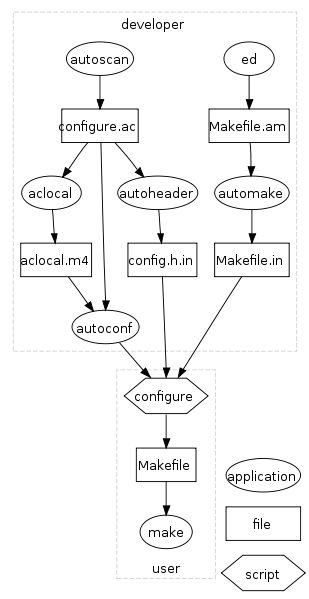
\includegraphics[scale=0.7]{pics/autotool1} \\	
			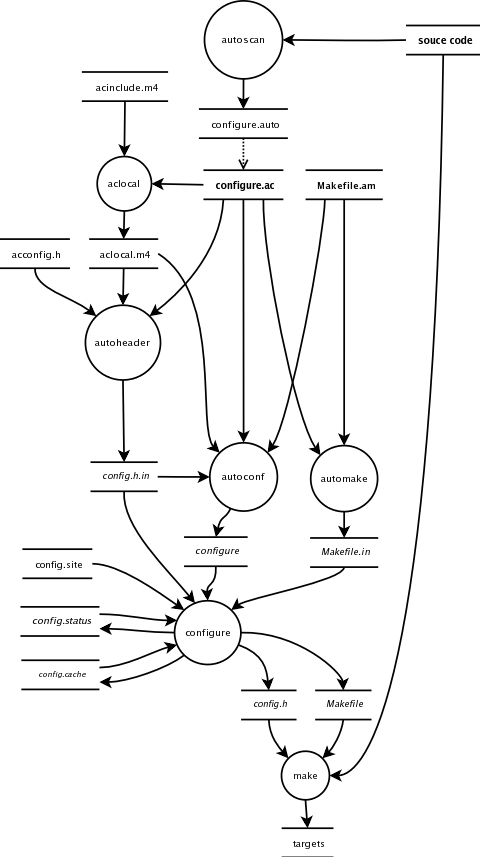
\includegraphics[scale=0.7]{pics/autotool2} \\	
		
		\item  Basic steps:
		\begin{enumerate}
		\item create project

         \item autoscan, then rename configure.scan ==> configure.ac
         \item aclocal
         \item autoheader( optional, it will produce config.h.in. But if you use AC\_CONFIG\_HEADER, you must run it.)
         \item Makefile.am(If you have multi-deep directory, make sure each directory has one)
            \item libtoolize –automake –copy –force(if configure.ac use libtool)
           \item automake –add-missing
           \item autoconf, it will produce configure command
           \item build another build\_dir, parallel with source project
            \item cd build\_dir. Then ../source/configure --prefix=/home/yan/install
            \item make \&\& make install
            	
		\end{enumerate}
			
				
		\item I have add some good reference paper to ref directory. When you really need them, just read them first. 

		\item By now, it support VPATHS, you can download source code, then make build1 subdir inside, then cd build1 sub, run ../configure, it will put all obj,bin and lib file in build1 sub directory. if you want to build another version. make build2 subdir inside, then run ../configur --different-conf. You can use the same set source code in this way. 
\end{itemize}
\subsubsection{config.ac}
\begin{itemize}
\item A example configure.ac

\begin{verbatim}
#                                               -*- Autoconf -*-
# Process this file with autoconf to produce a configure script.

AC_PREREQ([2.69])  
#must have 
AC_INIT([Hello], [0.3], [zhaoyan.hrb@gmail.com]) 
#change it 
AC_CONFIG_SRCDIR([config.h.in])
# Test if configure.ac is in the right directory

AC_CONFIG_HEADERS([config.h]) 
#use config.h to customize you source code

AC_CONFIG_MACRO_DIR([build-aux/m4]) 
# move your local m4 macro to target machine
# to avoid portable problem

AM_INIT_AUTOMAKE([foreign])
#use foreign, don't need README... five files.

case $host in 
    cpu-*-os*)
        COMP="aaa bbb"
       
        ;;
    *)
        COMP="ccc"
        
        ;;
esac
# ../src/configure --host=cpu-yan-os 
AC_SUBST(COMP)
# COMP will be aaa bbb, then use AC_SUBST to replace 
# COMP in the Makefile.am , "SUBDIRS = $(COMP)"
# in this way, aaa bbb will be compiled, otherwise, 
# ccc subdirectory will be built


# Checks for programs.
AC_PROG_CXX
AC_PROG_AWK
AC_PROG_CC
AC_PROG_CPP
AC_PROG_INSTALL
AC_PROG_LN_S
AC_PROG_MAKE_SET
## AC_PROG_RANLIB

AC_ARG_ENABLE([ember_paths],
[  --enable-ember-paths    cross-compile for EmbeR.],
[case "${enableval}" in
  yes) ember_paths=true ;;
  no)  ember_paths=false ;;
  *) AC_MSG_ERROR([bad value ${enableval} for --enable-ember-paths]) ;;
  esac],[ember_paths=false])
AM_CONDITIONAL([EMBER_PATHS], [test x$ember_paths = xtrue])

LT_INIT
# use libtools, detail can seen in libtools section

CXXFLAGS='-std=gnu++1y -g -O0'
# You can set users variable for make here.

# Checks for libraries.
AC_CHECK_LIB([lib1], [fun1])

# Checks for header files.
AC_CHECK_HEADERS([fcntl.h stdlib.h])

# Checks for functions.
AC_FUNC_MALLOC
AC_CHECK_FUNCS([gethrtime gettimeofday])

# Checks for typedefs, structures, and compiler characteristics.
AC_CHECK_HEADER_STDBOOL
AC_C_INLINE
AC_TYPE_INT64_T
AC_TYPE_MODE_T
AC_TYPE_SIZE_T
AC_CHECK_TYPES([ptrdiff_t])

AC_CONFIG_FILES([Makefile
                 src/Makefile
                 src/aaa/Makefile
                 src/bbb/Makefile
                 src/ccc/Makefile
                 ])
#which make file you want to produce.                 
                
AC_OUTPUT
\end{verbatim}
\item Main function of congiure.ac is to check lib, function and header file in the target system, then give error or config.h. In the end, you source code can custimize its behavior accordingly.

\item Another function is to set some variable, such as CXXFLAGS.

\item configure what subdirectories to be built on the different platform. In another word, what Makefile should be produced.

\end{itemize}

\subsubsection{Makefile.am}
\begin{itemize}
\item For recursive directory, each directory should have Makefile.am. on parent directory, just set "SUBDIRS = sub1 sub2"

\item use libtool to produce .so
\begin{verbatim}
AM_CXXFLAGS = -Wall -fPIC
if SWITCH
AM_CXXFLAGS += -fprofile-arcs -ftest-coverage
endif
//For ENABLEGCOV, you can use to 
../src/configure --enable-switch to turn on it.

lib_LTLIBRARIES = libyan.la

libyan_la_SOURCES =		\
	src1.cpp					\
	src2.cpp					\
	
AM_CPPFLAGS = -I$(top_srcdir)/src/includes 

libyan_la_LDFLAGS = -version-info 0:0:0 -L/usr/local/lib -L$(ODDS_LIBS)
libyan_la_LIBADD = -llibabc 
\end{verbatim}

\item produce .exe
\begin{verbatim}
include $(top_srcdir)/common.am
bin_PROGRAMS = exe1

exe1_SOURCES =						\
	main.cpp 							\
	init.cpp							

exe1_CPPFLAGS = -I$(top_srcdir)/src/includes 
exe1_LDFLAGS = -L/usr/lib64 -L/usr/local/lib64 
exe1_LDADD = -lboost_log -lboost_log_setup  
\end{verbatim}

\item For bin, lib, include, they are position. PROGRAMS LIBRARIES and HEADERS, they are categories. So for "bin\_PROGRAMS", it means that I want to produce an executable file and the executable file will be in bin directory.

\item include\_HEADERS means that this file will be installed in include directory.
\item A simple picture \\
   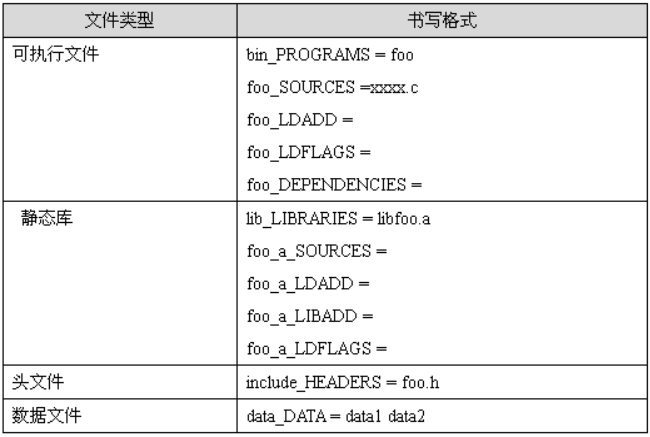
\includegraphics[scale=0.7]{pics/am} \\
\end{itemize}

\subsubsection{libtools}
\begin{itemize}
\item libtools is mainly used to produce .so file for different OS.
\item configure.ac and Makefile.am also support it.

\item In makefile.am use lib\_LTLIBRARIES, not lib\_LIBRARIES(that is used to build static library.)

\item How to compile a .so? See automake.am example in the previous section.
\item How to use a .so? You can use .la file directly in you automake.am. Pay attention to the two points: compile .so you need to use \_LIBADD to specify dependency. when you use .so you need to use\_LDADD to specify .so dependency. At the same time. .so will be baked into exe with rpath, so you can run your main directly. Don't need to set LD\_LIBRARY\_PATH varaible.
\begin{verbatim}
bin_PROGRAMS = main.c
main_LDADD = /path_to_la/libabc.la 
#la is special file extension of libtool
\end{verbatim}

\item A good introduction file can be found in "use GNU Libtool build lib" by wuxiaohu in Chinese version.

\end{itemize}

\subsection{CMAKE}
\begin{itemize}
		\item The best way to study is see a simple and complete template file. You can google "most simple but complete cmake example" and take a look.  

\end{itemize}

\section{git}

\subsection{Basic knowledge}
\begin{itemize}
\item \emph{A basic rule:  For single person, always pull (fetch and merge) before you work,  commit and push after you work.  For multi person, fetch and merge even before each commit.  Maybe other people have committed a new version on the remote repository. }

\item Run \linuxcommand{git gc} every month to run it to optimize.

\item In Linux, you can \linuxcommand{sudo apt-get install git-all} and meld(merge tools), In windows, you can download msysGit and P4Merge. You need edit your .gitconfig file, showed in the next section. you can use meld or P4Merge to visualize conflicts in source code. In Mac, you can download git from git home website. or install Xcode, when you install Xcode, It will install git in /usr/bin. but it will not install gitk GUI tool, so you can download git from home website and install another git on /usr/local/bin directory and use gitk in this directory. 

\item The two characteristics about git is \textbf{Distribute} and \textbf{Branch}, Distribute support working offline, Branch can make you manage branch easily and efficiently.

\item You need to know a few important conceptions: repository, branch, commit, paths and files. You need to know object of a command, such as merge command, it needs two branch. not two commits. Checkout branch will switch to its branch, and checkout commit will cause detached-head, etc.  
   
\item \textbf{origin} is a repository, \textbf{master} is a branch, \textbf{HEAD} is a ref to a branch. A repository can have many branches, so you can use origin/master to specify one of them. A branch can have many commits, so you can use HEAD\^{} to refer to it.
    
\item You also need to know some low-level knowledge about git. such as commit-->tree-->blob,  commit. You can use \linuxcommand{git log} to know the sha value, then use \linuxcommand{git cat-file -t (or -p) sha} to check them. 
    
\item you can use commit --allow-empty to produce a lot commits to use as test. then use \linuxcommand{rebase --keep-empty } to learn how to change history. Only some practical usage can teach you some knowledge. For Git , Dirty Hand is very very important.
        
        \item checkout and merge are different, checkout is used to \textbf{overwrite present with history}, merge is used to \textbf{combine present with history}.  

         \item When a command can be followed by <paths>, then <paths> can be:
				 \begin{enumerate}
						 \item a file 
							\item *.ext  Only current level directory, not recursive child directory.
							\item . (all file) All files recursively under child directory.
							\item /path\_name(path\_name and recursive) 
							\item /path\_name/*(no recursive). 
					\end{enumerate}
			\item When you read manual, you need to know, the same command has different usage when followed by different objects. For example, when checkout followed by a branch name, followed by a commit or followed by a <paths>, detail can be seen in git book p103.  reset followed by <paths> or followed by a commit is also different, detail can be seen git book p96. The main points is \textbf{checkout commit with path will change HEAD ref, and reset without path will change branch ref(such as master).}
         
         \item You need to understand difference between tree-ish and commit-ish. commit-ish can be used as tree-ish, but tree-ish can't be used as commit-ish. 
		 \item git cat-file and git show-ref are two useful commands, show-ref can give you big pictures of whole git project, and cat-file can help you to see deeply into each sha value. Detail information can be found in git document.                 
\end{itemize}

\subsubsection{git configure}
    \begin{itemize}

  \item \linuxcommand{git config -e [--global|system]}  -e will open a editor. --global means user, --system means /etc/.gitconfig.   If you omit options, It just produce a .gitconfig file for this repository. (local) Most of time, you don't have right to write in --system level. 

\item It's a social website, you need to find some friends here and exchange idea. The first thing you should do is to tell other peoples who you are.  
\begin{verbatim}
git config --global user.name "zhaoyan"
git config --global user.email zhaoyan.hrb@gmail.com
\end{verbatim}

    \item In windows, .gitconfig will be saved in  \\
    C:$\backslash$Documents and Settings$\backslash$Administrator directory.
    \item \linuxcommand{git config --global core.editor notepad} (use notepad as default editor)
    \item git config --list list all the configuration command options
 

\item  ~/.gitconfig template file, it will customize your own git behaves. (color and log alias is more useful). By now, I didn't use git very often, so I didn't give shorter alias name to each command.

\begin{verbatim}
[alias]
co = checkout
ci = commit -s   ## -s means to add name and email. Important when working with others.
st = status
br = branch
oneline = log --pretty=oneline --since='2 days ago'
onelog = log -p -1
[color]
status = auto
branch = auto
ui = auto
\end{verbatim}

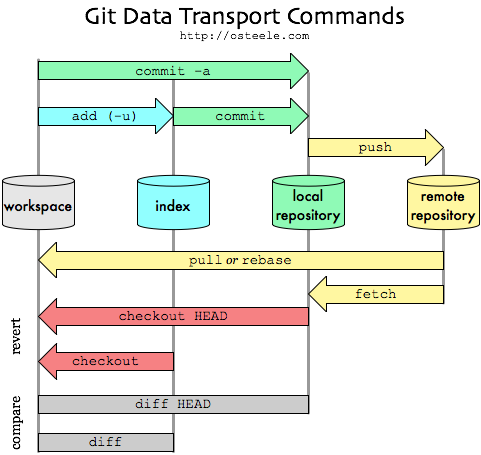
\includegraphics[scale=0.6]{pics/git-transport} \\

   \end{itemize}

\subsubsection{GitHub or gitlab}
\begin{itemize}
\item For gitHub, I have two github account:
\begin{enumerate}
  \item zhaoyan.hrb@gmail.com  zhaoyan;
  \item yan.zhao.74@gmail.com YanZhao
\end{enumerate}
A project hello-world, Main project is on zhaoyan, then I use YanZhao account fork main project. project link is : \\
git://github.com/zhaoyan/hello-world.git(read only) \\
git@github.com:zhaoyan/hello-world.git(modifiable)


\item \linuxcommand{ssh-keygen -t rsa -C yan.zhao.74@gmail.com} 

\item Your public key has been saved in /c/Users/zhao/.ssh/id\_rsa.pub(for windows) ~/.ssh/(for Linux). Then you should paste the public key to the account in github.com.  
        	
\item You can copy id\_rsa.pub and id\_rsa to other computers. so you don't need to run ssh-keygen command any more. But when you copy id\_rsa to linux or Mac, you need \linuxcommand{chmod g-r id\_rsa} to make your private key only readable for youself. Or when you push or fetch, git will refuse your request.  (ssh -v will give you verbose information. You must restart ubuntu after you move id\_rsa to ~/.ssh).


\item once you finish it, \linuxcommand{ssh -T git@github.com} will test you key setting. (github has details explanation.)

\item In your .ssh directory, if you find a id\_rsa file, don't change it. Because this file maybe used to connect some remote server. You can build or modifiy config file in ~/.ssh diectory. Add something below. 1) you can use your own id\_rsa\_old name here, how to use ssh-keygen to product different name, you can see manual. 2) \textbf{Don't add Port 443 statment first, if you use ssh -T to get no response, then add Port 443, then it will work}.
\begin{verbatim}
Host github.com
   Hostname ssh.github.com
   Port 443
   IdentityFile ~/.ssh/id_rsa_old
\end{verbatim}

    \item Sometimes, you can't see project link, you can click the little eye(watchers) on the right upper corner. pull request will show up.

\item \textbf{Don't use any Chinese in version control, If your English is not good, use Pinyin.}
    
\item In order to do anything in Git, you have to have a Git repository. This is where Git stores the data for the snapshots you are saving. There are two main ways to get a Git repository. \textbf{One way} is to simply initialize a new one from an existing directory, such as a new project or a project new to source control. \textbf{The second way} is to clone one from a public Git repository, as you would do if you wanted a copy or wanted to work with someone on a project.
\end{itemize}

\subsubsection{GUI}
\begin{itemize}
	\item There are two main GUI usages in git: 1) gitk 2) gui diff and merge    

    \item gitk is GUI application. gitk --all will list all the branches.

    \item For git diff and git merge commands, you can use some gui tool. For Linux, meld is the best option. You need to change you .gitconfig to add [diff] and [difftool] section. Pay attention. They finish the same task. Make you \linuxcommand{gui difftool} invoke the GUI diff(merge) application. You need to configure in this way. For mergetool, You should select one of two options. Usually, It will put your local workspace file left, and you merged branch right. and middle is your last result. I prefer to put \$BASE in the middle. But you can change it in your .gitconfig anytime. 
\begin{verbatim}
[diff]
    tool = meld
[difftool]
	prompt = false
[difftool "meld"]
	cmd = meld "$LOCAL" "$REMOTE"
[merge]
    tool = meld
[mergetool "meld"]
	path = /usr/bin/meld
	keepBackup = false
	trustExitCode = false	
# Choose one of these 2 lines (not both!) explained below.
	cmd = meld "$LOCAL" "$MERGED" "$REMOTE" --output "$MERGED"
    cmd = meld "$LOCAL" "$BASE" "$REMOTE" --output "$MERGED"
\end{verbatim}
       
      \item For Mac, I haven't test if meld can be used. But I have tried diffMerge, On its website, you can find how to config .gitconfig file.Detail can be found in diffMerge website. I will not duplicate it.

      \item For diff, you will not change git diff command. Only git difftool invoke GUI. For Merge, git merge just modify your file in work space to diff format when there is conflict. Then you need to run \linuxcommand{git mergetool} to invoke GUI application.  Just remember: \textbf{First run git merge, if conflict, then git mergetool}

\item When you run \linuxcommand{git mergetool} Meld will open three panel windows. Middle one is your result. left and right are two conflict branches.  When you finished. just click save and exit. Then run \linuxcommand{git status}, you can see it is ready for to add and commit. 
 
\end{itemize}

\subsection{Basic commands}
\subsubsection{status log show}
\begin{itemize}
		\item \linuxcommand{git status}  you need to use this command very often. 
		\item  \textbf{\linuxcommand{git status -uno} will not show untracked files.} \linuxcommand{git log --author=Bob} only show Bob's commit.

		\item \linuxcommand{git status -s} show two columns , the first is staging, the second is working tree. if you modify a file,  then add. then you modify a file again. Now git status -s show MM a. guess what it means?

	\item \linuxcommand{git log} can show you all the commits history. 

\begin{verbatim}
git log --pretty=oneline #just show simply log information
git log -p   #show ci log and source modification each commit.
git log -2  #just last two commits
git log --after 2015-12-01  #show all commits after date
git log --oneline  #simple informaitons
git log --abbrev-commit --pretty=oneline #simple informaitons
git log experiment..master #show commits on master, not on experiment
        a--b--e--f(master)
            \c--d(experiment)
git log origin/master..HEAD #what have you push to remote?
\end{verbatim}

   \item \linuxcommand{git show} to examine a single object. such as \linuxcommand{git show v1.0} and\linuxcommand{git show master:book.tex} will output source file.  It can used on commit(just like log command), or tree (just like cat-file -p). or plain blobs,(just like cat-file -p). 
 \end{itemize}

\subsubsection{add commit}
\begin{itemize}
		\item When you add, You should know:
				\begin{enumerate}
						\item There is tree in index, but we don't give this tree a sha value, 
						\item For any new added file, produce a blob object, and assign a sha value to it, and add it to tree object.
						\item For any added file, produced new blob object, because sha has changed. Updated tree object.
						\item When you commit, give a tree sha value, and copy whole tree out, add tree object to commit object, and give commit object a sha value.
				\end{enumerate}

		\item You can use \linuxcommand{git status -uno} to hide all untraced files. You also can produce a \textbf{.gitignore} file in you project, it will work on present and all children directory. When you use \linuxcommand{git status}, It will not show many untracked files.  Example is below. edit .gitignore file.

\begin{verbatim}
# comment
*.a   #ignore all files with .a extention
!lib.a  #but include lib.a
build/   #ignore all file in build directory
doc/*.txt  #ignore all txt files in doc/ but doc/server/arch.txt will be included.
\end{verbatim}

		\item You should avoid using \linuxcommand{git add .} to add so many unnecessary files. If you run it accidentally,  You can use \linuxcommand{git reset} to revert add which you just ran. Or you can use \linuxcommand{git rm -r --cached .} to delete it from index, but keep file in working directory.

\item When there are a lot of files to add, \linuxcommand{add -i} is a good choice.  \linuxcommand{add -u} will only add tracked files, no dot is needed. 

\item Current working directory is (1),   Index file or staging is (2) and  Git local repository is (3) \\
      (1) -> (2) -> (3) \\
  \linuxcommand{git add} (1) -> (2) \\
   \linuxcommand{git commit} (2) -> (3) \\
   \linuxcommand{git commit -a}  (1)->(3) Don't recommend use it. \\

    \linuxcommand{git add .}   add all files. Be careful to use this command   \\
    \linuxcommand{git add -u}   it's very often used command. or It can be used in such situation: rm *.txt, then git add -u will delete *.txt from staging. \\
    
    \item commit command usually don't pay attention to files or directory, it just product a commit to produce a sha object(commit). 

   \item \linuxcommand{git commit --amend}  don't produce new commit, just modify last commit. But it will change previous commit sha value. 
   
   \item If you add a file a.c, but you don't commit it. How to revert? \linuxcommand{git reset a.c} Will remove a file named a.c from the current index, the "about to be committed" area, without changing anything else.  contrary to  \linuxcommand{git add --a.c} To undo git add . use git reset (no dot).
   
   \item If you haven't commit yet, so you can't use reset now. At this time you can use \linuxcommand{git rm --cached} command, then commit it again. 
   
   \item Previous method will produce two commits. if you want to just modify current commit.  git rm first, then use \linuxcommand{git commit --amend}.  Or you can also use \linuxcommand{git reset HEAD~}, then maybe you need git add or not, depends on your context. last \linuxcommand{git commit -c ORIG\_HEAD}.  Here reusing the old commit message. reset copied the old head to .git/ORIG\_HEAD; commit with -c ORIG\_HEAD will open an editor, which initially contains the log message from the old commit and allows you to edit it. If you do not need to edit the message, you could use the -C option. \textbf{This method only reuse old commit message, not very useful in my view point}

   \item Both(commit --amend) and (reset... commit again) will produce new commit. In fact, any commit sha include current operation second will be different. 
   
   \item \textbf{So don't change commit which you pull from public or you have pushed to public} 
        
		\item You can use \linuxcommand{git ls-files -s} to see all files in the index and their corresponding sha value.
		\item You can use \linuxcommand{git ls-tree -l HEAD} to see all files in the HEAD commit.
\end{itemize}

\subsubsection{remove rename}
\begin{itemize}
		\item Basic command:
\begin{verbatim}
git rm a // It will delete from work space and index
git rm --ached a  //just delete a from index.
git commit -m "delete file a"

git mv a b  #is three command: mv a b; git rm a ; git add b ;
git commit -m "rename a to b"
\end{verbatim}
		\item git rm will delete file from working directry, git rm --cached will only delete file from index. \textbf{They have nothing with commit}
		\end{itemize}

\subsubsection{diff}
\begin{itemize}
\item diff basic usage. Usually, you should follow a file name after diff command. 

\begin{verbatim}
git diff     ##(1) and (2)
git diff -cached   ##(2) and (3)
git diff HEAD   ##(1) and (3)

git diff tag     ##tag and HEAD
git diff tag file    ##just compare a file (only one file name)
git diff tag1..tag2   ##two tags( you can omit two dots)
git diff SHA11..SHA12  ## two commits
git diff tag1 tag2 file or  git diff tag1:file tag2:file

#tag can be a alias of remote
git remote add xjsff git://github.com/xjsff/hello-world.git
git diff xjsff/master README  ##local README and README in xjsff/master
\end{verbatim}
		\item \linuxcommand{git diff --name-only} just show changed files name. so you can compare it one by one.  \linuxcommand{git diff --name-status} will show how do you changed files, add, delete or modify. 

		\item Before checkout or reset, you'd better to use diff command to see if there are important content to avoid overwrite. that is a good habit. 

		\item diff -u is good command, it will show context of difference.  All the differences give by differences section.
   
\item  After git fetch, you can use \linuxcommand{git diff master origin/master} to see all the modifications, then decide if you want to merge. fetch+merge is better than pull.
   
\item \linuxcommand{git difftool -- file} to use meld to see the difference, it looks much better.
\end{itemize}
\subsubsection{checkout reset}

\begin{itemize}
		\item \textbf{branch->commit, HEAD->branch, When not follow paths, checkout move HEAD, reset move (HEAD->branch, HEAD must point to a branch). } It's helpful for you to understand these two command.
		
		\item If HEAD->master, reset will move HEAD->master together, if HEAD->commit, reset will only move HEAD. at this time, It's still detached head status. 
		
		\item There are two basic different usages for checkout: 
		\begin{enumerate}
		\item with paths(file), it just with <commit> to replace index and work space. At the same time, It will not change HEAD. 
		\item without paths, if you follow a branch it will move HEAD to branch.
		\item without paths, if you follow a old <commit>, It will move HEAD to old <commit>. HEAD will be a ref to a branch,  When It points a real old commit, It will be "detached HEAD" and all commits after HEAD may be discards in the future. 
		\item \linuxcommand{checkout <commit> -- paths} or \linuxcommand{checkout branch}. Don't use in\linuxcommand{git checkout <commit> (empty)} without paths, It will put HEAD in detached state. \textbf{After checkout, follow a branch, or follow /patth/file name.}
		\item \linuxcommand{git checkout} just like \linuxcommand{git status}
		\end{enumerate}
				
		\item When checkout and reset follow file, they can be a file, *.cpp(some files) , . (all files),  /path\_name(path\_name and recursive) and /path\_name/*(no recursive). 

	 \item If you are in detached HEAD state, 1)You don't modify work space, just use checkout master to set HEAD to master again. 2)If you modify work space and you want to keep it. commit it first, remember <commit-sha>. Then checkout master. merge <commit-sha>. Then HEAD will move to master and master will point to merged commit.  
	 
\item If there is no commit following the checkout command, only file, it will use file in index to overwrite work sapce. \linuxcommand{git checkout . or git checkout file} (2)->(1). 

\item If there is commit, \linuxcommand{git checkout HEAD .}  (3)->(1) and (2) dot represents all the files. \textbf{This is a dangerous command. Save or commit you local work first.}
    
\item \textbf{checkout will overwrite work space directly, it is not like merge, and doesn't produce conflict files. So be careful!}
 
\item you can checkout a file from different history. :
\begin{enumerate}
\item \linuxcommand{git checkout v1.2.3 -- filename}  tag v1.2.3 

\item \linuxcommand{git checkout stable -- filename}  stable branch 

\item \linuxcommand{git checkout origin/master -- filename}  upstream master 

\item \linuxcommand{git checkout HEAD -- filename}   the version from the most recent commit 

\item \linuxcommand{git checkout HEAD\^{ } -- filename}   the version before the most recent commit 

\item \linuxcommand{git checkout xxxx  --filename} xxxx is commit version number.
\end{enumerate}


\item  Similarly, There are two different usages for reset: 
\begin{enumerate}
\item with paths, it will not move HEAD and master (reset commit). \linuxcommand{git reset <commit>-- <paths or filename>} will overwrite index with commit, (3)->(2).  it just like contrary operation of add.

\item Without paths, it will reset (HEAD-->master) together to a new <commit>, and all commits after reset commit will be discards( delete commits, dangerous!). Because It reset (HEAD-->master) together, then It doesn't have detached head problem.  

\item Without paths, there are three options you can use:
\begin{verbatim}
git reset [--soft|hard|mixed ] <commit>
## soft just reset commit
## mixed reset commit and (3)-->(2)
## hard reset commit and (3)-->(2)-->(1)
\end{verbatim}
\end{enumerate}

\item How to save from wrong reset command? When you reset to a <old-commit>. All the commits after <old-commit> will not found easily unless you can remember all the commit sha value.  A better method can be use \linuxcommand{git reflog show master | head -5}. It will show master@{0...n}. It represent all the master ref history. You also can use it to show head moving history.      

\item HEAD@{num} can be used as follow to change commit history after a <old-commit>
\begin{enumerate}
\item \linuxcommand{git checkout <old-commit>} \# detached head
\item \linuxcommand{git commit ...} \#last commit sha is 123abc
\item \linuxcommand{git checkout master} \# move head to branch
\item \linuxcommand{git reset --hard HEAD@{1}} \# reset it to old commit 123abc.  
\end{enumerate}

\item followed by <old-commit>, both checkout and reset --hard will modify all files in work space. 

\item If you modify a file in (1), you can restore it from (2) with \linuxcommand{git checkout --a.c} or from(3) with \linuxcommand{git checkout HEAD --a.c}.  They will overwrite (1) forever, so be careful. If you want to keep it, you can do:

\end{itemize}
\subsubsection{tag}
\begin{itemize}
\item push tag to remote.
\linuxcommand{git push origin <tag\_name>}
And the following command should push all tags (not recommended):
\linuxcommand{git push --tags}
\end{itemize}
\subsubsection{stash}
\begin{itemize}
		\item Sometimes I have a situation that I am working on some feature on my own branch and suddenly someone comes to me and says that something really important has to be fixed or improved on the main branch. Usually it happens when I am in the middle of very important changes which are not ready to be committed for some reason. 

\item Normally, I would have to save the changes (diff) into some file, switch to the main branch abandoning any changes, apply the fix or improvement and commit it. Then I could switch back to my own branch, apply the changes (patch) from the file and continue the work. While it is not something difficult, it can be done much easier with Git.

\item When you use \linuxcommand{git stash}, It will run \linuxcommand{git reset --hard} automatically. so all you work will disappear. you can use \linuxcommand{git statsh pop }to revert it.
\item stash will save both working and index.
\item stash will only save files which have added to index.
\item \textbf{After stash, system will call reset --hard HEAD automaticlly, so if you have new files, you'd better add it to index before you use stash command.}
\begin{verbatim}
You need to modify a bug in release version. First stash, then checkout release. coding....,commit,last git stash pop.
git stash save "you messaage" #
git stash list #list all stash
git statsh pop #
\end{verbatim}

\end{itemize}

\subsubsection{rebase revert}
\begin{itemize}

\item Reverting has two important advantages over resetting. First, it doesn't change the project history, which makes it a "safe" operation for commits that have already been published to a shared repository. For details about why altering shared history is dangerous, please see the git reset page.

\item Second, Git revert is able to target an individual commit at an arbitrary point in the history, whereas git reset can only work backwards from the current commit. For example, if you wanted to undo an old commit with git reset, you would have to remove all of the commits that occurred after the target commit, remove it, then re-commit all of the subsequent commits. Needless to say, this is not an elegant undo solution.

\item revert will produce a new commit too. \verb=git revert HEAD^^ = produce a new commit

\item \textbf{Never rebase branches or trees that you pulled. Only rebase local branches.  Never ever rebase a branch that you pushed, or that you pulled from another person}

\item rebase command steps: git rebase master
\begin{enumerate}
\item now you are in branch1, 
\item All changes made by commits in the current branch but that are not in master are saved to a temporary area.
\item reset --hard master
\item The commits that were previously saved into the temporary area are then reapplied to the current branch, one by one, in order.
\end{enumerate}
\item You can ommit the --onto, it will 

\item rebase command and merge command is little different. \textbf{When you are in test branch, master branch has a new commit, You can rebase on new commit on master. Because in the end, your test branch will be merged back to master, rebase often can save you a lot of conflict problem in the future. }

\item \textbf{When you in the master branch, and When test branch has finished or partly finished, You can use git merge command to merge test branch into master branch}

\item You can think merge and rebase are two commands operate on branch.

\item rebase basic usage.
1) in master  branch , commit a new commit (m1), in test branch, commit few times(t1..t2). \\
\begin{verbatim}
   t1-->t2
 /
m-->m1
\end{verbatim}
2) checkout test branch, then \linuxcommand{git rebase master.} /* means that SHA value has been changed.\\
\begin{verbatim}
       t1*-->t2*
      /
m-->m1
\end{verbatim}

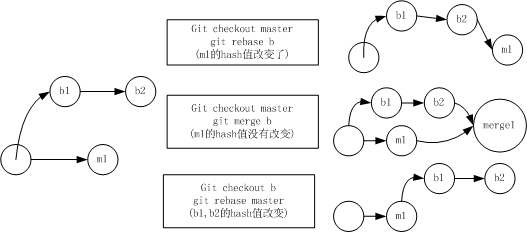
\includegraphics[scale=0.7]{pics/Git_rebase} \\

\item rebase has --onto options. Detail can be found in git rebase document. Just google it. 

\item rebase branch1 means 1) you are not in branch1 now 2) branch1 is melding point, 3) all commits value will be changed. 

\item You can use rebase on current branch, in this way, you want get clean history, and most of time, you use it with -i option. 
\item You can use rebase to rebase your branch work on master branch. it's another usage of rebase. 

\end{itemize}


\subsubsection{remote push pull fetch}
\begin{itemize}
		\item Fetch is not just a child command inside of pull, from result, you can think that "pull = fetch + merge". But, in fact, Fetch is extract all the remote branches to local. It's configured in remote subsection in .git/config

		\item origin is local alias of remote repository url. You can see it in .git/confg file.  

\begin{verbatim}
[remote "origin"]
	fetch = +refs/heads/*:refs/remotes/origin/*
	url = git@github.com:zhaoyan/new_doc.git
\end{verbatim}
				
\item For push and pull, you have to make sure you are in one branch, and it will only push and pull one branch from remote. 

\item You have to make sure local branch tracking the remote one. In anoter word, for a branch, you should see a config content in .git/config
\begin{verbatim}
[branch "master"]
	remote = origin
	merge = refs/heads/master
\end{verbatim}
\item Now, if there is branch on remote, you can first fetch, then git checkout -b local-branch-name remote-branch-name. In this way, a configure content will be added to .git/config automaticlly, and you local-branch will track remote one.
\item track means that when you in local-branch, you can run push and pull without any argument to syncronize local and remote branch.

\item If have a local branch, but remote doesn't have one. You have two ways:
\begin{enumerate}
		\item If you git version is greater than 1.7, then you can use git push -u origin <branch>. -u is important option, and if you want to change branch name, you can use loca-name:remote-name sytastic trip.
		\item If you use old version, use git push origin branchB, then add below to .git/config file
\begin{verbatim}
[branch "branchB"]
    remote = origin
	merge = refs/heads/branchB
\end{verbatim}
\end{enumerate}

\item don't use pull, just use fetch, then merge.  When you run \linuxcommand{git merge origin/master master}, there are three possibilities. 
		\begin{enumerate}
				\item Working directory no modification, then fast-ward merge and working and index will be updated. 
				\item Working directory has modification, merge will fail. 
				\item Working directory has modification and commit, merge maybe ok, then working and index will be updated. merge maybe conflict, then use merge tool to resolve conflict and commit to produce a commit manually.
		\end{enumerate}

\item origin is a alias of remote repository,  \linuxcommand{git remote add origin git@github.com:zhaoyan/test.git}just give a alias name, It will not real create remote repository, you need to log in github to create it manually.  Beside add, you can show, rename and delete a these alias. with these alias, you can \linuxcommand{push or fetch origion} directory, don't need to write the address of the remote repository.

\begin{verbatim}
git remote add paul git://github.com/paul/test.git
git remote -v
git remote show paul #show paul all the informations, including branch.
git remote rename paul pa
git remote rm pa #delete pa, because he will not contribute the system.
\end{verbatim}

\item push command is followed by a repository name and a branch name.  such as \linuxcommand{push origin master}. It has a lot of syntax, can be use change remote branch name and delete remote branch.
\begin{enumerate}
\item git push origin experiment \#push a branch to server
\item git push origin local:experiment \#change local branch name, and push to server. 
\item git push origin :experiment \#delete local branch ,use empty name 
\item git push origin erperimental:experimental-by-yan \#give remote-tracking-branches other name,here experimental-by-yan is remote-tracking-branches name,erperimentallocal name. <source-name>:<destination-name>
\end{enumerate}

\end{itemize}


\subsection{History}
\subsubsection{history representation}
\begin{itemize}
\item No space in tag name.
\item Common used history commit ref name list: 
\begin{verbatim}
ORIG_HEAD, COMMIT_EDITMSG
HEAD, MERGE_HEAD, FETCH_HEAD

HEAD^: #HEAD's parent, it's ORIG_HEAD
HEAD^ or HEAD^1   # first parent
HEAD^^ or HEAD^2 # second parent
HEAD~4 : 

HEAD:README.txt #A file inside a commit
\end{verbatim}
\end{itemize}

\subsubsection{history change}
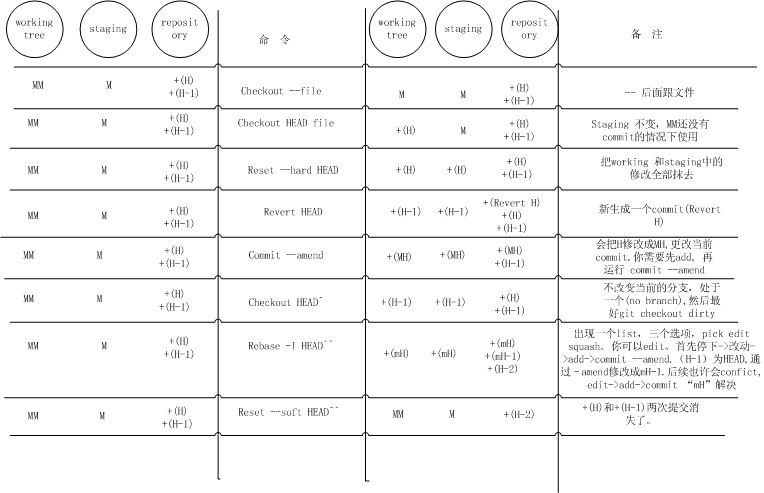
\includegraphics[scale=0.6]{pics/Git-history} \\
\begin{itemize}
\item \textbf{Three basic modification history usage:}
\begin{enumerate}
\item Delete or combine certain commits;
\item Delete new commits after a point
\item Delete old commits before a point
\end{enumerate}

\item \textbf{Three common commands for modifying history: checkout, cherry-pick and reset. Other useful command is rebase, you can think that it's a combination of previous three commands. Detail can be seen in rebase command}

  \item \textbf{Change current latest commit} \linuxcommand{git commit  --amend} not only change the message, but also the working tree contents. 
    
  \item revoke latest commit.
\begin{verbatim}
git commit -m "Something terribly misguided"              (1)
git reset HEAD~                                           (2)
<< edit files as necessary >>                             (3)
git add ...                                               (4)
git commit -c ORIG_HEAD                                   (5)
\end{verbatim}
\begin{enumerate}
\item This is what you want to undo
\item This leaves your working tree (the state of your files on disk) unchanged but undoes the commit and leaves the changes you committed unstaged (so they'll appear as "Changes not staged for commit" in git status and you'll need to add them again before committing). If you only want to add more changes to the previous commit, or change the commit message1, you could use git reset --soft HEAD~ instead, which is like git reset HEAD~ but leaves your existing changes staged.
\item Make corrections to working tree files.
\item git add anything that you want to include in your new commit.
\item Commit the changes, reusing the old commit message. reset copied the old head to .git/ORIG\_HEAD; commit with -c ORIG\_HEAD will open an editor, which initially contains the log message from the old commit and allows you to edit it. If you do not need to edit the message, you could use the -C option.  \textbf{-c option is just reuse last time commit message}
\end{enumerate}

  \item \textbf{Delete some new commits} \linuxcommand{git reset --hard  HEAD\^{}\^{}\^{}} will delete \verb=HEAD^^=  and \verb=HEAD^=  and HEAD three commits forever, It's is a dangerous command, be careful about it.
   
\item \textbf{Delete all old commits before A} 
\begin{enumerate}
\item \linuxcommand{echo "Commit from tree of tag A" | git commit-tree A\^{}\{tree\}}  It will produce a <SHA value>. This command will produce a new commit with <SHA value> and without any parent. It's a root commit. 

\item \linuxcommand{git rebase --onto <SHA value> A master}  All the history behind of A will be deleted. 
\end{enumerate}


  \item \textbf{Delete some old  commits by cherry-pick } 
 \begin{enumerate}
\item \linuxcommand{git checkout C}, C is a tag, by now, working tree is C status, Here, you can't use \linuxcommand{reset C}, because it will put master to C,  then D, E and F will not be accessed. 
\item \linuxcommand{git cherry-pick E and F} , delete D commit ,cherry pick will produce a new commit SHA value, such as E* and F*. 
\item \linuxcommand{git checkout master }  It will end Head detached status. 
\item \linuxcommand{git reset --hard HEAD@\{1\}}. reset HEAD-->master to new F* commit. 
 \end{enumerate}

  \item \textbf{Delete some old commits by rebase } 
 \begin{enumerate}
\item \linuxcommand{git rebase --onto m1 m2 m5}, You need to know that  m2 m5 will not include m2, It will produce a new commit m3, m4 and m5,
   SHA value will be different. And from the figure, you can see that master branch is still on old m5 commit.  so you need perform step 2. 
\begin{figure}
  \centering
    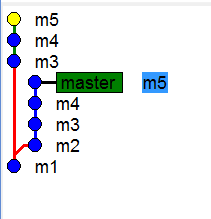
\includegraphics[scale=1.0]{pics/rebase1}
\end{figure}


\item \linuxcommand{git rebase --onto m1 m2 master} will keep you track master branch, after that you don't need to run step 2 below. It will be easy way to do that. 

\item \linuxcommand{git checkout master }  and \linuxcommand{git reset --hard HEAD@\{1\}}. After these two commands, you can see m2 has disappeared. 
\begin{figure}
 \centering
  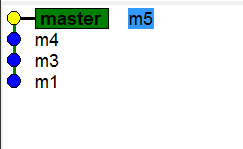
\includegraphics[scale=1.0]{pics/rebase2}
\end{figure}
 \end{enumerate}
  
  \item \textbf{Combine two old commits by cherry-pick} 
 \begin{enumerate}
 \item \linuxcommand{git checkout D}, by now, working tree is D status,  
\item \linuxcommand{git reset --soft B } ,  because HEAD is D now, go to B, --soft means working tree is still D status 
  \item \linuxcommand{git commit -C C }  then \linuxcommand{git cherry-pick E and F}. 
 \item \linuxcommand{git checkout master }  \linuxcommand{git reset --hard HEAD@\{1\}}. Detail can be found in "Got Git". 
 \item \textbf{It will not produce conflict, just delete a commit, if you want to delete modification inside a commit, maybe it will produce conflict}.
 \end{enumerate}


\item \textbf{Combine two old commits by rebase} 
\begin{enumerate}
\item \linuxcommand{git checkout D}, D is a tag, by now, working tree is D status, 

\item \linuxcommand{git reset --soft B } ,  because HEAD is D now, go to B, --soft means working tree is still D status 
\item \linuxcommand{git commit -C C }  
\item \linuxcommand{git tag newbase} \textbf{give a tag name to avoid remember sha-value} \\
\item \linuxcommand{git rebase --onto newbase D master}  then check \linuxcommand{git branch }to see if it's on branch master, if it's yes 
\item \linuxcommand{git tag -d newbase } 
\item  Detail can be found in "Got Git". 
\end{enumerate}
 

\item \textbf{difference cherry pick and rebase} 
\begin{enumerate}
\item rebase and cherry pick will change commit SHA value, so don't use it on any commit that you have pulled or you have pushed. cherry pick will not change 

\item cherry pick should be used in change few commits, and rebase can be used to change a lot of commits at the same time.  
\end{enumerate}

\item \textbf{delete all the commits in a merged branch}
\begin{enumerate}
\item \linuxcommand{git rebase -i} will open an editor, then you can give some commands inside this file. the name of this file is git-rebase-todo file.

\item git rebase -i will run it according to this file. 

\item git rebase -i <sha before the branches diverged> this will allow you to remove the merge commit and the log will be one single line as you wanted.  Detail can be seen rebase command. 

\item A detail can be seen in google "squashing commits with rebase"

\end{enumerate}

\end{itemize}

\subsubsection{blame} 
    \begin{verbatim}
    git blame -L l2,l3 hello.html
    \\Who made some modification.
    \end{verbatim}


\subsection{Branch}
\subsubsection{Basic conception}

\begin{itemize}
\item Usually, there are three common use branches. One is release branch which can be based on one release commit. Usually, it used to fix some bugs in release, then you can merge back master branch. Another is feature branch, when you add a feature, and you don't know if it's good or can be finished properly, you can produce a feature branch. At the same time, keep master branch keep growing.

\item Feature branch is usually based on current HEAD,  and release branch is usually based on one release tag.  So you need to build a tag first.

\item After you finish your Feature branch or Release(bug fix) branch. There are two options, if only you work on the branch, such as Feature branch, you can merge it back to master branch, and push master to remote. 

\item Or if other people also need this branch, such as Release branch, you need to push it to remote, so other people can update their own work according to your work.  How to push local branch to remote and keep track-able, see remote section.

\item \textbf{For Release branch, you should switch back master, and pick or merge commits in Release branch back to master branch}

\item \textbf{For Feature, branch, If developing-time is short, just merge it back master, and push master to remote. If developing-time is long, At this time, There is new commits on master, at this time, you should pull back master, and perform rebase command}.
		
\item If you project is based on other work, you also need vendor branch. You don't commit on it. just keep track with upstream new version , then merge back with you master branch.

\item when you want to merge others work, you'd better build a branch first.

\item Branch is based on commit,  When you merge a branch back to  master, you may delete it if you don't need it anymore. 

\item For branch, you can undo a merge commit, or you can delete all the commits in one branch after you have merge. Detail can be seen in section History
\end{itemize}

\subsubsection{Branch command}
\begin{itemize}
\item checkout -b can be thought as short hand of two commands 1) branch create a new branch, and 2) checkout to switch it. 

\begin{enumerate}
\item \linuxcommand{git branch -r}  list all the branches on the remote
\item \linuxcommand{git branch}  list all the local branches
\item \linuxcommand{git branch -D b1}  delete the b1 branch forcefully
\item \linuxcommand{git branch -m master mymaster} rename the branch

\item \linuxcommand{git checkout -b new-branch master} new-branch based on master and switch to it.
\item \linuxcommand{git checkout -b new-branch} build new-branch based on current branch.

\item \linuxcommand{git checkout branch-name} switch to branch-name
\end{enumerate}

  \item merge command is followed by two branches, no files name.  such as \linuxcommand{git merge origin/master master}
  
  \item Three merge results:
  \begin{enumerate}
\item Fast-Forward merge, You don't need run commit it. 
  \item without conflict merge,  git will produce a new commit automatically.
  
 \item conflict merge , Git will not resolve conflict for you. it will put working tree into a specify conditions. (file in work space has been modified with conflicted format). you need manually resolve it.
  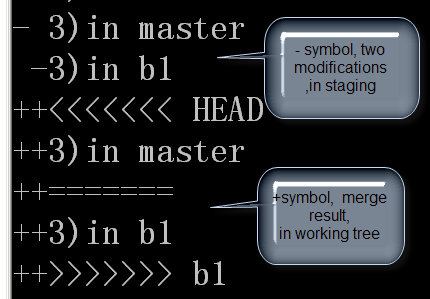
\includegraphics[scale=0.6]{pics/merge-diff} \\
After you resolve conflict, run git add file-name and git commit.

\item You can see figure below to understand it better. \\
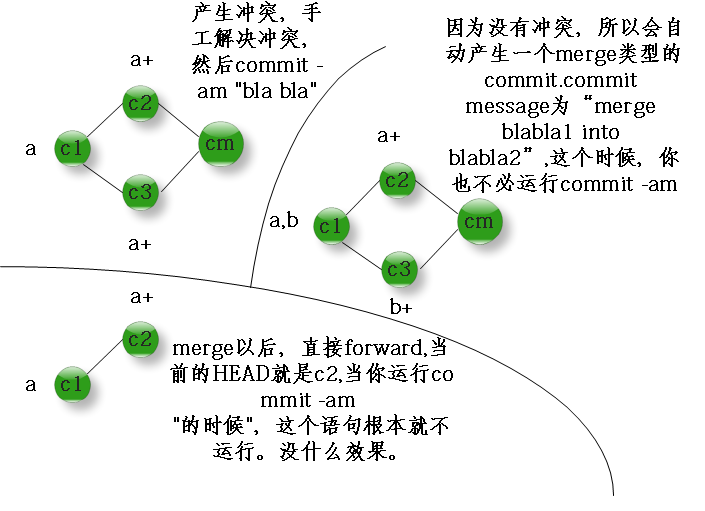
\includegraphics[scale=0.5]{pics/git-merge} 
\end{enumerate}

\item Three kinds of merge:
\begin{enumerate}
\item straight merge. Merge all the commits in one branch into another.

\item squash merge. Change all history into one commit. \linuxcommand{git merge --squash contact}. You need merge first, then commit.
\begin{verbatim}
git checkout master
git merge --squash bugfix
git commit
\end{verbatim}

\item cherry-pick. git cherry-pick 32176f(another commit in other branch). or git cherry-pick -n 32176f, which n means that you don't want commit immediately. When you git commit later, without m, then editor will open, all cherry you picked commit message will be in this editor. 
\end{enumerate}

\item \linuxcommand{git merge-base b1 b2}  found the common ancestor

\item \linuxcommand{git cherry -v master test}  In master branch, found all commits in test, but not in master.

\item You've already committed the merge that you want to throw away, use this command: \linuxcommand{git reset --hard ORIG\_HEAD}.



\end{itemize}


\subsubsection{Remote Branch}
\begin{itemize}
\item Branch can be in two different positions. One is in the local place, you can use git branch to check them. The other is remote-tracking branches, you can use git branch -r to check them. The name format is "origin/remote-branch-name", origin is not branch name, it's repository name. About how to synchronize local and remote branch? and how to make local branch is track-able with remote branch. you can see remote subsection.

\item You can't checkout remote branch, such as \linuxcommand{git checkout origin/branch1}. In order to do so , you have to create a local branch based on remote branch, such as \linuxcommand{git checkout --track -b branch1 origion/branch1}, then work on the local branch1. after you finish it, you can push it back. with --track, you can push or fetch without specify remote repository name. --track option can be omitted here. 

\item \linuxcommand{git checkout -b new-branch origin/new-branch} build new-branch based on origin/new-branch. And add track ability.  In this way, If you are in the local new-branch, you can push and pull directly. 
\end{itemize}

\subsubsection{Branch daily usage }
\begin{itemize}
\item Single person, center control, with branch. When you finish the branch, you can merge it with master. 

\item Below figure show two different position are working on the same branch--malouf. \\

	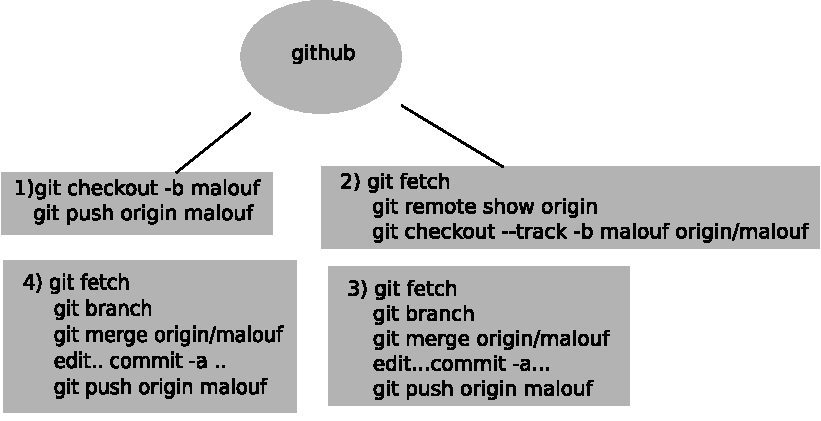
\includegraphics[scale=0.6]{pics/git_branch} \\
   
\item Multi person, center control, with branch 

   \begin{enumerate}
     \item \linuxcommand{git fetch upstream} get zhaoyan upstream the updated development process.
     \item \linuxcommand{git checkout -b test\_bla upstream/master} based zhaoyan master branch, build local branch test\_bla (any name is OK.)
     \item edit,  compile, \\
     git commit -am "s1" \\
     edit,  compile,  \\
     git commit -am "s2"\\
     While, upstream/master maybe changed,  a new commit t1 appear.
\begin{verbatim}
     s1--- s2
____/___t1
\end{verbatim}
\item \linuxcommand{git fetch upstream} when you want to update upstream, you have to get new commits

\item \linuxcommand{git merge upstream/master} If no conflict, produce a forward merge, if conflict, manually
    resolve and commit a new commit. \linuxcommand{git commit -am "st1"}
\begin{verbatim}
      s1--- s2
____/___t1___\st1__
\end{verbatim}

\item Or,\textbf{A more recommended method is} you can use the second method: \linuxcommand{git rebase upstream/master} No conflict, produce a new commit. with conflict, manually resolve it, then \linuxcommand{git add conflict\_file}, then
    \linuxcommand{git rebase --continue}, not need to commit.
    \begin{verbatim}
        t1---s1*--- s2*
____/
\end{verbatim}

\item git push origin test\_bla

\item login github, look for you repository, checkout test\_bla, then click "request pull" button.

\item If other accept you request, you can delete test\_bla branch. \linuxcommand{git branch -D test\_bla}

\item \linuxcommand{git push origin  :test\_bla}  delete test\_bla branch in github.
\item  repeate 1-10.
   \end{enumerate}
\end{itemize}

\subsection{conflict}
\begin{itemize}
		\item In git, there are a lot of commands will cause conflict, such as revert, merge, cherry-pick,rebase and so one. If you see document, you will find all comand are with --continue and --abort command options.

		\item \textbf{All command will perform three-way merge command, It will merge two commit based on two commit common ancestor.}

		\item c1 is commit 1, c2 is commit 2, and A is common ancester. Basic idea is use diff command to produce diff format information from A to c1. such as "2d1", which represent delete the second line in A and produce c1, in c1 there is only one line.  Also produce diff format information from A to c2, such as "2a3,4", which represent from the second line in A, add another two line in c2. Then if two diff bot include number "2", it means that there is conflict, you need to resolve it manually. 

		\item From previous explanation, When you consider if it will conflict, you should not only consider c1 and c2, you should consider their common ancestor and a serical diff format information. 

		\item For merge and rebase command, common ancerstor is very clear. but for some command, such as revert and cherry-pick, common ancestor is not very clear. You can think common ancestor is older(c1, c2)-1 commit is their common ancestor.  
		
\end{itemize}

\subsection{Daily usage}
\subsubsection{Clone a project from github}
\begin{enumerate}
\item  \linuxcommand{git clone git@github.com:zhaoyan/hello-worl.git}  you can copy the address from github website. I think that it will produce origin alias automatically.
\item modify... main.cpp
\item \linuxcommand{ git add main.cpp}  \linuxcommand{git commit  -m "modify sth..."}
\item \linuxcommand{ git log} to see if you have commit successfully.
\item \linuxcommand{git remote -v } to see what origin is.
\item \linuxcommand{git push origin master }   This command works only if you cloned from a server to which you have write access and if nobody has pushed in the meantime. If you and someone else clone at the same time and they push upstream and then you push upstream, your push will rightly be rejected. You'll have to pull down their work first and incorporate it into yours before you'll be allowed to push. detail can be seen in the previous push command: produce non-fast-forward error.
\end{enumerate}

\subsubsection{Add a project to a git}
\begin{enumerate}
  \item \linuxcommand{cd test}, run \linuxcommand{git init}
  
  \item \linuxcommand{touch test.cpp}, then \linuxcommand{git add test.cpp} or \linuxcommand{git add .}. dot means all the files. Directories are added automatically when adding files inside them. That is, directories never have to be added to the repository, and are not tracked on their own. You can say "git add <dir>" and
 it will add all files in there.
 
  \item \linuxcommand{git rm README}  you can delete a file
  
  \item \linuxcommand{git commit -m "first commit" } or \linuxcommand{git commit -a -m "first commit"} This is simple form. Combine add and commit together. Git commit -a can't add new files. If you add some news files, you should use \linuxcommand{git add newfile}. then commit.

\item \linuxcommand{git log} or \linuxcommand{git status} After committing, you can use log command to check if it has been submitted successfully.

\item \textbf{Then, login github, create repository with name test}

\item \linuxcommand{git remote add origin git@github.com:YanZhao/test.git}
		
\item \linuxcommand{git remote -v }you can check remote repository
\item \linuxcommand{git push -u origin master} 	You can not emit origin, if you don't specify branch, default is master. master is default local branch, you don't need to create it explicitly. this command push local content to the server.
\end{enumerate}


\subsubsection{Update a project from github}
\begin{enumerate}
\item  \linuxcommand{git clone git@github.com:zhaoyan/hello-worl.git}  you can copy
    the address from github website.
\item modify... main.cpp
\item \linuxcommand{ git add main.cpp}  \linuxcommand{git commit  -m "modify sth..."}
\item \linuxcommand{git log} to see if you have commit successfully.

\item \linuxcommand{git fetch}  to get origin/master.

 \item \linuxcommand{git diff master origin/master} maybe you need to resolve conflict before you push.
 
\item \linuxcommand{git merge origin/master} If there are difference, you need to merge before you push, or it will produce non-fast-forward error.  default is local master branch, you can't write in "git merge master" to skip "origin/master".

\item \linuxcommand{git push origin master}

\end{enumerate}

\subsubsection{Collaborate With Applications}

\begin{itemize}
  \item For codeblock, project file is pro1.cbp, It will produce two directory bin and obj, you need to modify .gitignore file, add bin/ and obj/ to ignore. good suggestion.
  \item For kdevelop:
 \begin{enumerate}
\item rm Makefile.in or .svn (if there are) 
\item go into the src directory, and run git init 
\item git add . and  git commit 
\item git remote add origin git@github 
\item git push origin master 

\item another kdevelop, rm src
\item git clone git@github src
\item modify Makefile.am with you kdevelop project file.
\item in configure dialog, Configure options->linker flager -> add -L./ and add lib to the debug/src directory.
\item compile and run.
\end{enumerate}  

  \item For latex,  Only *.tex *.bib( reference)  and /pic directory are useful, You need to add them manually.
\end{itemize}

\subsubsection{single person on different computers }
On computer 1:
\begin{enumerate}
    \item \linuxcommand{git log HEAD..origin}  to check if there are differences. if true
    \item \linuxcommand{git fetch,  git merge origin/master master} ( git fetch give you more chance to examining it, it's better than pull)
    \item \linuxcommand{git commit -a -m " "}
    \item \linuxcommand{git push}
    \item  \linuxcommand{git log HEAD..origin }check push successfully
\end{enumerate}

On Computer 2: \\

Same operation, when you merge, it will only produce forward merge, it's relatively easy.

\subsubsection{cooperation}
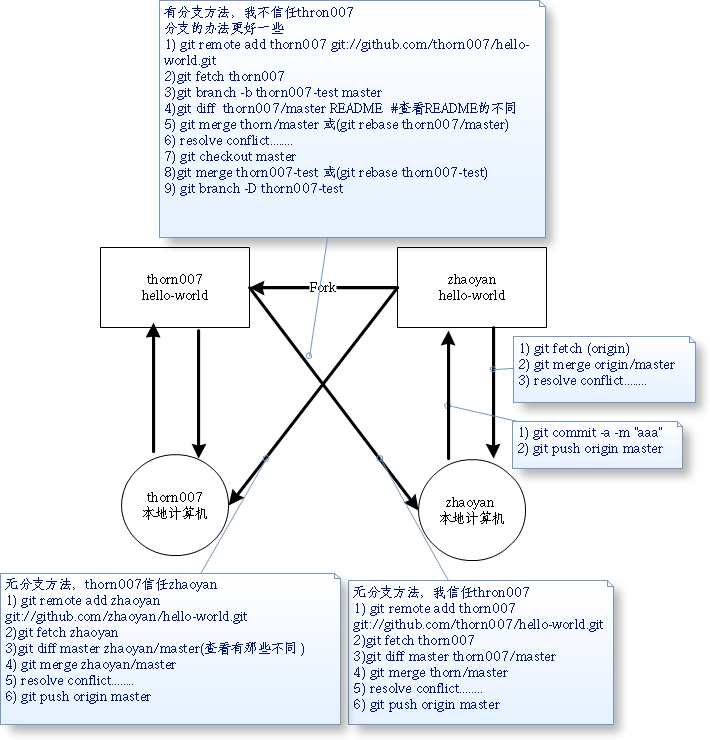
\includegraphics[scale=0.8]{pics/git-corp} \\

% \begin{verbatim}

%
% 下面我给出一个具体的例子:
% 当合作伙伴bob希望改进我(rocrocket)的工作成果,则:
% $git clone /home/rocrocket/project myrepo //此命令用于克隆我的工作到bob的myrepo目录下。请注意,此命令有可能会因为/home/rocrocket的目录权限问题而被拒绝,解决方法是chmod o+rx /home/rocrocket。
% (省略bob数小时的开发过程)…
% $git commit -a //bob提交自己的改进成果到自己的git仓库中,并口头告知我(rocrocket)他已经完成了工作。
%
% 我如果非常信任bob的开发能力:
% $ cd /home/rocrocket/project
% $ git pull /home/bob/myrepo //pull命令的意思是从远端git仓库中取出(git-fetch)修改的代码,然后合并(git-merge)到我(rocrocket)的项目中去。读者要记住一个小技巧,那就是“git pull .”命令,它和git merge的功能是一样的,以后完全可以用git pull .来代替git merge。请注意,git-pull命令有可能会因为/home/bob的目录权限问题而被拒绝,解决方法是chmod o+rx /home/bob。
%
%
% 如果我不是很信任bob的开发能力:
% $ cd /home/rocrocket/project
% $ git fetch /home/bob/myrepo master:bobworks //此命令意思是提取出bob修改的代码内容,然后放到我(rocrocket)工作目录下的bobworks分支中。之所以要放到分支中,而不是 master中,就是要我先仔仔细细看看bob的开发成果,如果我觉得满意,我再merge到master中,如果不满意,我完全可以直接git branch -D掉。
% $git whatchanged -p master..bobworks //用来查看bob都做了什么
% $git checkout master //切换到master分区
% $git merge bobworks
% $git branch -D bobworks //如果我检查了bob的工作后很不满意,就可以用-D来放弃这个分支就可以了
% 过了几天,bob如果想继续帮助我开发,他需要先同步一下我这几天的工作成果,只要在其当初clone的myrepo目录下执行git pull即可:
% #git pull //不用加任何参数,因为当初clone的时候,git已经记住了我(rocrocket)的工作目录,它会直接找到我的目录来取。
% \end{verbatim}
	\begin{itemize}
	\item if modification is small , you can use email+patch; If the modification is big, you can use fork pattern

    \item you can clone a exist project from others people or on other computers,
	\item Use email topic
		\begin{verbatim}
		1) git clone http://www.bitsun.com/git/gittutorcn.git
		2) edit and commit
		//method 1 (develop on master)
		$ git  fetch origin
		$ git rebase origin
		$ git format path origin  ->0001-your-buddy-s-contribution.txt
		//method 2 (develop on branche, better)
		$ git checkout -b patch_mubs
		$ git checkout master
		$ git pull
		...
		$ git checkout patch_mubs
		$ git rebase master ( why I need rebase here, I want to know answer)
		
		3)email 0001-your-buddy-s-contribution.txt to vortune@gmail.com
		for vortune:
		1) git checkout -b buddy-in
		2) git am /path/to/0001-your-buddy-s-contribution.txt
		
		\end{verbatim}
	\end{itemize}

    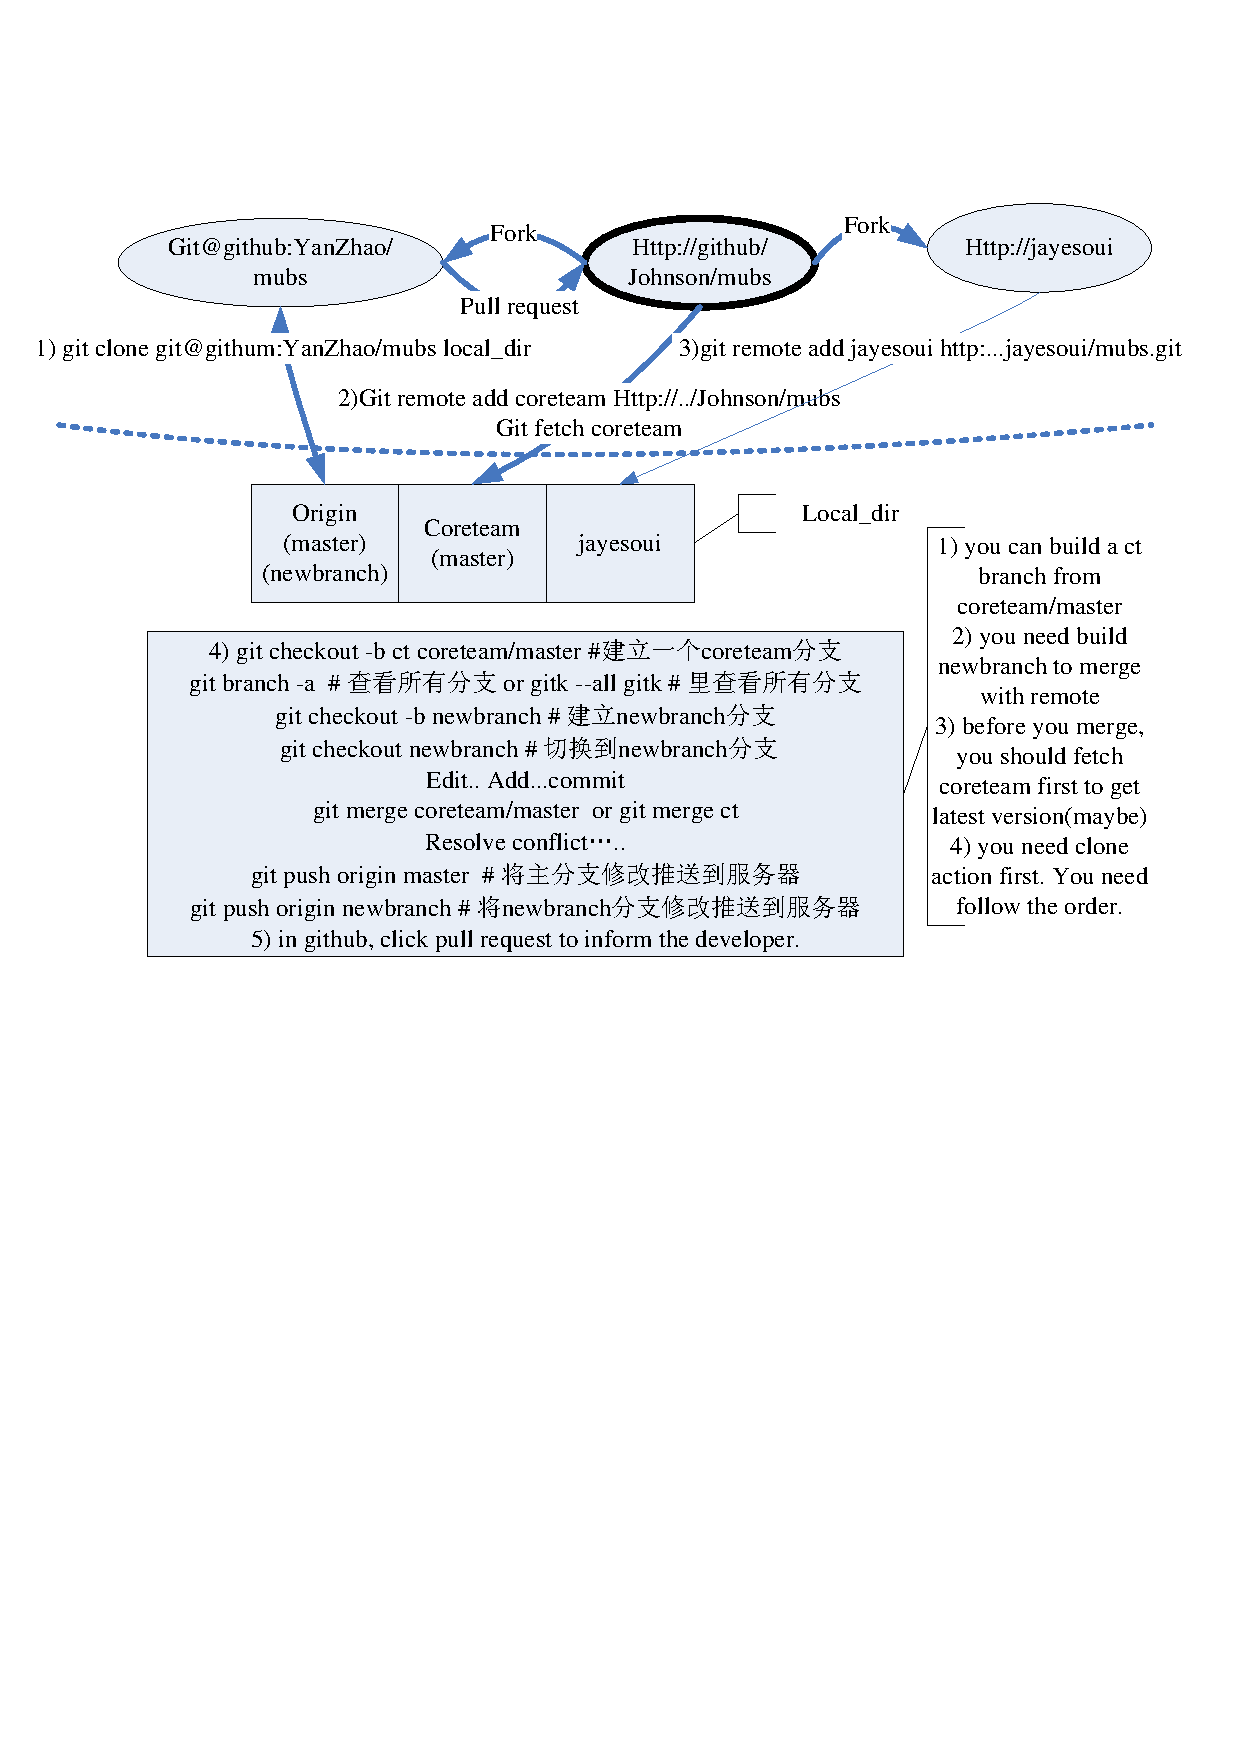
\includegraphics[scale=0.7]{pics/Visio-git_cooperate}



\section{IDE}
If you can access GUI, you can use code::block and kile to develop and documents. if
you login by SSH, By now, I think that best tool is Emacs, with GUD, it can debug a
program. Does Emacs support latex well? Yes, It has tex mode. \par

Windows has VS community version.  Mac has Xcode, but I didn't try it too much. 

In linux, There are many tools you can uses. The most advance tool is Eclipse. the medium tools are codelite and UltraGDB. And the simple tool is vim and gdb( gdb -tui) \\

ddd is old tool, when I use it in mint 17, It's difficult to set font.  It seems that a bug for ddd. and ddd is old tool which seems to stop developing.  \\

Then I try affinic debugger, It's a commercial software and need serial number, I look for and there is not many answers on google, Maybe it's not very popular,  and the shortcoming is white background and you cann't change color theme. so I give it up. \\

codelite is a good tool, Setting->colours and fonts->Customize->C++ , you can select Themes: Monokai\_2, and you can set font MonoSpace 11pt.  
in codelite, you need to set terminal as gnome-terminal in Setting->preferences->terminal "/usr/bin/gnome-terminal -t '\$(TITLE)' -e '\$(CMD)'"
It also use xterm as debugger output. In mint, it output ugly font.  you need to produce .Xresources file on you home directory.  I keep it on the linux software backup. 

UltraGDB is subset of Eclipse, if you just need front-end of GDB, It's the best one. You can set dark theme in Window->Preferences->General->Appearance \\

In conclusion,  front end of GDB are UltraGDB and codelite. IDE are eclipse and codelite.

\subsection{Understand}
Understand is a good tools to read a large scale software. 
\begin{itemize}
\item Don't add .h, .inc, or .inl files into understand project, It will be included by .cpp and analyze automatically. 
\item For C++, use strict option in project configuration. You can adjust c++ version in strict C++ configuration. By now, It's good to use C++11, C++14 is too new
\item In Understand ,you can use "Improve project accuracy"->"missing include files" to help you search head file automatically. 
\item For CMake file, you can use \textbf{CMake -CMAKE\_EXPORT\_COMPILE\_COMMANDS -G "Unix Makefiles"} It will produce a compile\_commands.json file. In the end, you can use \linuxcommand{und} to produce a project.und. It will includes correct configuration information.  Don't use -G "Xcode", It will not produce  compile\_commands.json file.  Detail can be seen in my EverNote bookmark. 
\item For gcc and g++ project, you can use buildspy tool in Understand, detail can be seen in my EverNote bookmark.
\item If you select "terminal" color theme, inactive code will not visiable, you can change the background color to make it visible through "Preferences"->"Editor"->"Styles"
\item When analyze a long or difficult file, "worker process killed after 2 mins", you can try "Ananlyze changed file " again. if 2 minutes is too short, you can configure it longer on this specify file by override configuration. 
\item Macro is key factor in understand project, you can define it maually, but recommended way is to use CMAKE or buildsyp or visual studio to prodce a understand project automatcilly. it will includes all the correct Macro defination and include path. 
\item You can use buildspy to build a understand project in linux, configure project to relative path "Portability" then you can move source code and understand project to Mac, and use understand in Mac to open it. the interface on Mac looks better than Linux. 

\item By now, I have two projects, one is llvm and the other is openuh.  For llvm, when you run CMake in test1 directory, It will produce some head file, when you compile use xcode or makefile, It will produce some def file. But I didn't run can compiling in test1 directory, but I have really compiled src in cmake\_release\_build directory. When i use add automaticlly search headfile, it add some files in cmake\_release\_build directory. In Understand Project Browers, you can see these three directories, in fact, test1 and cmake\_release\_build are overlapped. 

\item for LLVM and openuh, when you configure and compile the source code, It will produced some addtional files to be used in compiling in build directory. so, In the end you understand project will also include build directory in the end. 
  
\end{itemize}





\chapter{Other Tools}






\section{OS and phone}

\subsection{useful tips}
\begin{itemize}
\item In linux or mac, if you want to print c++ source with linenumber, you can use \\
\verb=enscript -MLetter --line-numbers -p - --word-wrap a.cpp | pstopdf -i -o ~/out.pdf=
you can use \verb=brew install enscript= to install enscript. Maybe you will see a error: you can't write /usr/local/etc.
then use \verb=sudo chown -R `whoami`:admin /usr/local/share=to give you permission. and then try brew again. 
\end{itemize}

Common used applications in each OS. in phone, I didn't install many app by now. it make you phone battery die very quickly. and I always sit in front of computer. \\

\begin{tabular}{|c|c|c|c|}
\hline & mac & windows & linux  \\
\hline diagramming & \parbox[c]{10em}{\centering OmniGraff \\ ConceptDraw}& visio & Dia   inkscape \\
\hline vector drawing & illustrator & coreldraw illustrator & ? \\
\hline edit & textmate & Ultraedit & Emacs \\
\hline doc & mactex & Ctex & livetext \\
\hline web & dreamweaver & dreamweaver & ? \\
\hline screenshot & jing snapZ pro & snagit & ? \\
\hline screencast & \parbox[c]{10em}{\centering screen flow \\ camtasia }& camtasia & Xvidcap \\
\hline download & amule or Vuze & emule & amule  \\
\hline audio editor & \parbox[c]{10em}{\centering audacity(amateur) \\ logic(profession)} & \parbox[c]{10em}{\centering gold wave(amateur)\\ adobe audition(professional)} & ? \\
\hline video editor & \parbox[c]{10em}{\centering finalcut \\  imoive(amateur)} & \parbox[c]{10em}{\centering premiere(professional) \\HuiShengHuiYing (amateur)}& ? \\
\hline
\end{tabular}
\subsection{Phone}
\begin{itemize}
  \item In my phone, weibo, webchat and web browser are three information sources.
  \item Evernote is main note tool. It can sync between phone and computer. When you have a lot note in Evernote, you can import them to latex document if you have time.
  \item In phone, you can use Everclip, on computer, you can use Evernote web clipper( in chrome browser)
  \item In Weibo or Webchat, you can repost or share it on moment. That is very easy way to keep knowledge. If this knowledge is just useful for you, you can use Everclip text, download image, or copy URL, Then use share function in your phone to save them to Evernote.
\end{itemize}
\subsection{mac}
\begin{itemize}
 \item command is window key if you use a windows keyboard.
 \item command+~ switches between documents. command+tab switches between applications.
  \item quicksiver can open and close any applications
  \item homebrew can be used to install a lot soft package from git to /usr/local/bin. It's very easy just brew install. 
  if you have older version in /usr/bin, you need to export PATH=/usr/local/bin:\$PATH. It's not very convenient. For this problem, you can down load module software, and use module load and unload, it is  environment management . 
  \begin{verbatim}
  brew install modules 
  \end{verbatim}
  
  \item 
  \begin{tabular}{|p{0.45\textwidth}|p{0.45\textwidth}|}
  \hline command +T & open a new brower \\
  \hline command+T, command + ~ & switch application or windows \\
  \hline command+shift+4 & screen snap \\
  \hline command+option+esc & force app quit(you need to command+tab switch ) \\
  \hline command+h & hide current windows \\
  \hline command+Q or W & close app or windows. \\
  \end{tabular} 
  
\end{itemize}

\subsection{win7}
\begin{itemize}
\item win+arrow key can dock windows to left,right,maximize and minimize, that is very useful
\item win+p can control project camera
\item win+1,2,3 can launch programme in task bar quickly
\item when the explore becomes slowly, you should check tool--manager add-ons to see which add-on is slow.
\item right mouse key can produce a jump list, the content of jump list will change according to the type of progamme.
\item move windows to the left side can change it to 50\% width.
\item win+L to lock the windows
\end{itemize}

\subsection{iexplore and chrome}
\begin{itemize}
\item learn to use tab to explore the internet. that is very useful, don't try to open a new page in a new windows, but in a new tab. \hotkey{ctrl+num} to navigate the tabs. and \hotkey{ctrl+click} to open a link in a new tab. \hotkey{ctrl+T} open a new tab. \hotkey{ctrl+w} to close the current tab.
\end{itemize}






\ifx \allfiles \undefined
%\end{CJK*}


\end{document}
\fi
